\chapter{Analytical Solutions for Structure factors}
\label{sec:structurefactor}
The different types of structure factors can be selected in the
different submenus. Below one finds how they are ordered. The
definitions of the individual structure factors are defined below.
Under the submenu \texttt{other} all structure factors under
development and those functions, which are not structure factors
at all but which have been implemented for some other purposes are
listed.

\begin{itemize}
\item None
\item Hard \& Sticky Hard Sphere
 \begin{itemize}
 \item Hard Sphere
 \item Sticky Hard Sphere
 \item Sticky Hard Sphere 2
 \item Square Well Potential
 \item Square Well Potential 2
\end{itemize}
\item Multi Lamellar Structures
\begin{itemize}
 \item ThermalDisorder
 \item Paracrystalline
 \item ModifiedCaille
\end{itemize}
\item anisotropic obj.
\begin{itemize}
\item P'(Q): local planar geometry
\begin{itemize}
\item P'(Q):ThinDisc
\item P'(Q):ThinSphericalShell
\item P'(Q):ThinEllipsoidalShell
\item P'(Q):ThinHollowShell
\end{itemize}
\item P'(Q): local cylindrical geometry
\begin{itemize}
\item P'(Q):TinRod
\item P'(Q):SAW(withEXV)
\item P'(Q):SAW(withoutEXV)
\end{itemize}
\end{itemize}
\item fractal obj.
\begin{itemize}
\item Mass Fractal (Exp Cut-Off)
\item Mass Fractal (Gaussian Cut-Off)
\item Mass Fractal (Exp(-x$\hat{~}$a) Cut-Off)
\item Mass Fractal (OverlapSph Cut-Off)
\end{itemize}
\item other
\begin{itemize}
 \item Mass Fractal
 \item Cylinder (PRISM)
 \item VoigtPeak
 \item Correlation Hole
 \item Critical Scattering
 \item Macro Ion (HP)
 \item Local Order
 \item RandomDistribution
\end{itemize}
\end{itemize}

\section{Methods to include structure factors}
For each scattering object $i$ next to a size distribution $N_i(x;\B{l}_i)$ also a
structure factor $S_i(Q;\B{s}_i)$ can be included. When a structure factor is included
several theoretical ways to account for it have been implemented
like the monodisperse approximation (\ref{sec:SQmonodisperse}),
decoupling approach (\ref{sec:SQdecoupling}),
local monodisperse approximation (\ref{sec:SQlocalmonodisperse}),
partial structure factor (\ref{sec:SQpartial})
and scaling approximation of partial structure factors (\ref{sec:SQscaling}).
At the moment it is assumed that there are no interactions between different species
of scatterers so that the total scattering is given by the sum of the scattering of the
individual species
\BE
\frac{d\sigma}{d\Omega}(Q) = \sum\limits_{i=1}^N \frac{d\sigma_i}{d\Omega}(Q)
\EE
whereby different approaches to include structure factor effects in
the differential scattering cross-sections $\frac{d\sigma_i}{d\Omega}(Q)$
of the species $i$ of scatterer are defined below.

\subsection{Monodisperse approach}
\label{sec:SQmonodisperse}
~\\

The monodisperse approach is the simplest way to include a structure factor in the analysis.
This approach simply multiplies the size averaged form factor with the structure factor.
Here it is assumed that the interaction potential between particles are spherical symmetric
and independent of the particle size.

\BE \frac{d\sigma_i}{d\Omega}(Q) = \left[
\int_0^\infty N_i(x;\B{l}_i)
F_i^2(Q;\B{a}_i,x) dx \right] S_i(Q;\B{s}_i)
\EE

\subsection{Decoupling approximation}
\label{sec:SQdecoupling}
~\\

For systems with small polydispersities and small anisotropies leads to a
decoupling approach of Kotlarchyk and Chen \cite{Kotlarchyk1983}. It is assumed that interactions
are independent of particle size and orientation.
%\begin{subequations}
\begin{align}
\frac{d\sigma_i}{d\Omega}(Q) = &
\int_0^\infty N_i(x;\B{l}_i) F_i^2(Q;\B{a}_i,x) dx
+  \frac{1}{n_i}\left[\int_0^\infty N_i(x;\B{l}_i)
F_i(Q;\B{a}_i,x) dx\right]^2  \nonumber \\
\times & \left[S_i(Q;\B{s}_i)-1\right]
\end{align}
with
\BE
n_i = \int_0^\infty N_i(x;\B{l}_i)  dx.
\label{eq:ni}
\EE

The decoupling approximation can only be combined with those form factor,
for which the scattering amplitude $F_i(Q;\B{a}_i,x)$ has been implemented.
However, for many form factors only the scattering intensity $F_i^2(Q;\B{a}_i,x)$ is
available. The combination of those form factors with the decoupling approach produces
an error message in \SASfit.



\subsection{Local monodisperse approximation}
\label{sec:SQlocalmonodisperse}
~\\

The opposite limit of the approximations as used for the
decoupling approximation is used in the local monodisperse
approximation \cite{Pedersen1994}. In this approach it is assumed
that a particle of a certain size is always surrounded by
particles with the same size. Following this the scattering is
approximated by that of monodisperse sub-systems weighted by the
size distribution:
\BE
\frac{d\sigma_i}{d\Omega}(Q) =
\int_0^\infty N_i(x;\B{l}_i)
F_i^2(Q;\B{a}_i,x) S_i(Q;\B{s}_i,R_i(\B{a}_i,x)) dx
\EE
in which it has been indicated that the structure factor is for particles of size
$R_i(\B{a}_i,x)$. As the distribution $N_i(x;\B{l}_i)$ does not necessarily describe the
distribution of the overall size. \SASfit assumes, that the radius of a particle
with the form factor $F_i(Q;\B{a}_i,x)$ used in the structure factor is given
by the radius of a sphere with the same volume $V_i(\B{a}_i,x)$
\BE
R_i(\B{a}_i,x) = \oldsqrt[3]{\frac{3}{4 \pi}V_i(\B{a}_i,x)}.
\label{eq:Ri}
\EE
This local monodisperse approximation works better than the decoupling approximation for
systems with larger polydispersities and higher concentrations. As
compared to the decoupling approximation and the scaling
approximation described below, it has the advantage that the cross
section is linear in the size distribution.

\subsection{partial structure factors}
\label{sec:SQpartial}
~\\

For polydisperse systems it is also not possible to write the scattering cross section as a
product of a form factor and a structure factor. The scattering cross section has the form
%\begin{subequations}
\begin{align}
\frac{d\sigma_i}{d\Omega}(Q) =
&\int_0^\infty N_i(x;\B{l}_i) F_i^2(Q;\B{a}_i,x) dx \\
+ & \frac{1}{n_i}\int_0^\infty\int_0^\infty N_i(x;\B{l}_i)N_i(x';\B{l}_i)F_i(Q;\B{a}_i,x)F_i(Q;\B{a}_i,x') \nonumber \\
\times & \left[S_i(Q;\B{s}_i,R_i(\B{a}_i,x),R_i(\B{a}_i,x'))-1\right] dx dx' \nonumber
\end{align}
%\end{subequations}
where monodisperse structure factor $S_i(Q;\B{s}_i,\dots)$
is evaluated for the radius
$(R_i(\B{a}_i,x)+R_i(\B{a}_i,x'))/2$. $n_i$ and $R_i(\B{a}_i,x)$ have the same
definition as those in eq.\ \ref{eq:ni} and \ref{eq:Ri}.

\subsection{Scaling approximation}
\label{sec:SQscaling}
~\\

A scaling approximation has recently been introduced by Gazzillo
et al. \cite{Gazzillo1999}. It is assumed that the pair correlation functions
are identical except for a scaling constant. This leads to the
following expression:
%\begin{subequations}
\begin{align}
\frac{d\sigma_i}{d\Omega}(Q) =
 &\int_0^\infty N_i(x;\B{l}_i) F_i^2(Q;\B{a}_i,x) dx \\
+ & \frac{1}{n_i}\int_0^\infty\int_0^\infty
N_i(x;\B{l}_i) N_i(x';\B{l}_i) F_i(Q;\B{a}_i,x) F_i(Q;\B{a}_i,x') \nonumber \\
\times & \frac{\overline{V}_i(\B{a}_i,x,x')}{V_{i,av}}
\left[S_i(Q;\B{s}_i,R_i(\B{a}_i,x),R_i(\B{a}_i,x'))-1\right] \;dx
dx' \nonumber
\end{align}
%\end{subequations}
where $V_{i,av}$ is given by
\BE
V_{i,av} = \frac{\int_0^\infty N_i(x;\B{l}_i) V_i(\B{a}_i,x) dx}{\int_0^\infty N_i(x;\B{l}_i) dx}
\EE
and $V_i(\B{a}_i,x,x')$ by
\BE
\overline{V}_i(\B{a}_i,x,x') = \frac{4}{3}\pi \left(\frac{1}{2}\left(\oldsqrt[3]{\frac{3}{4\pi}V_i(\B{a}_i,x)}+\oldsqrt[3]{\frac{3}{4\pi}V_i(\B{a}_i,x')}\right)\right)^3
\EE
and the monodisperse structure factor is evaluated for the radius
$(R_i(\B{a}_i,x)+R_i(\B{a}_i,x'))/2$. $n_i$ and $R_i(\B{a}_i,x)$ have the same
definition as those in eq.\ \ref{eq:ni} and \ref{eq:Ri}.

Note that the expression is not linear in the size distribution
and that it involves double integrations, which makes least-square
fitting with this expression relatively slow.

\subsection{van der Waals one-fluid approximation}
\label{sec:SQvdW1}
~\\
This approximation is similar to the scaling approximation introduced by Gazzillo
et al. \cite{Gazzillo1999}. The exact formular is given by
%\begin{subequations}
\begin{align}
\frac{d\sigma_i}{d\Omega}(Q) =
 &\int_0^\infty N_i(x;\B{l}_i) F_i^2(Q;\B{a}_i,x) dx \\
+ & \frac{1}{n_i}\int_0^\infty\int_0^\infty
N_i(x;\B{l}_i) N_i(x';\B{l}_i) F_i(Q;\B{a}_i,x) F_i(Q;\B{a}_i,x') \nonumber \\
\times & \frac{\overline{V}_i(\B{a}_i,x,x')}{V_{i,x}}
\left[S_i(Q;\B{s}_i,R_i(\B{a}_i,x),R_i(\B{a}_i,x'))-1\right] \;dx
dx' \nonumber
\end{align}
%\end{subequations}
where $V_{i,x}$ is given by
\BE
V_{i,av} = \frac{\int_0^\infty N_i(x;\B{l}_i) V_i(\B{a}_i,x) dx}{\int_0^\infty N_i(x;\B{l}_i) dx}
\EE
and $V_i(\B{a}_i,x,x')$ by
\BE
\overline{V}_i(\B{a}_i,x,x') = \frac{4}{3}\pi \left(\frac{1}{2}\left(\oldsqrt[3]{\frac{3}{4\pi}V_i(\B{a}_i,x)}+\oldsqrt[3]{\frac{3}{4\pi}V_i(\B{a}_i,x')}\right)\right)^3
\EE
and the monodisperse structure factor is evaluated for the radius
$(R_i(\B{a}_i,x)+R_i(\B{a}_i,x'))/2$. $n_i$ and $R_i(\B{a}_i,x)$ have the same
definition as those in eq.\ \ref{eq:ni} and \ref{eq:Ri}.

Note that the expression is not linear in the size distribution
and that it involves double integrations, which makes least-square
fitting with this expression relatively slow.



\begin{figure}[htb]
\begin{center}
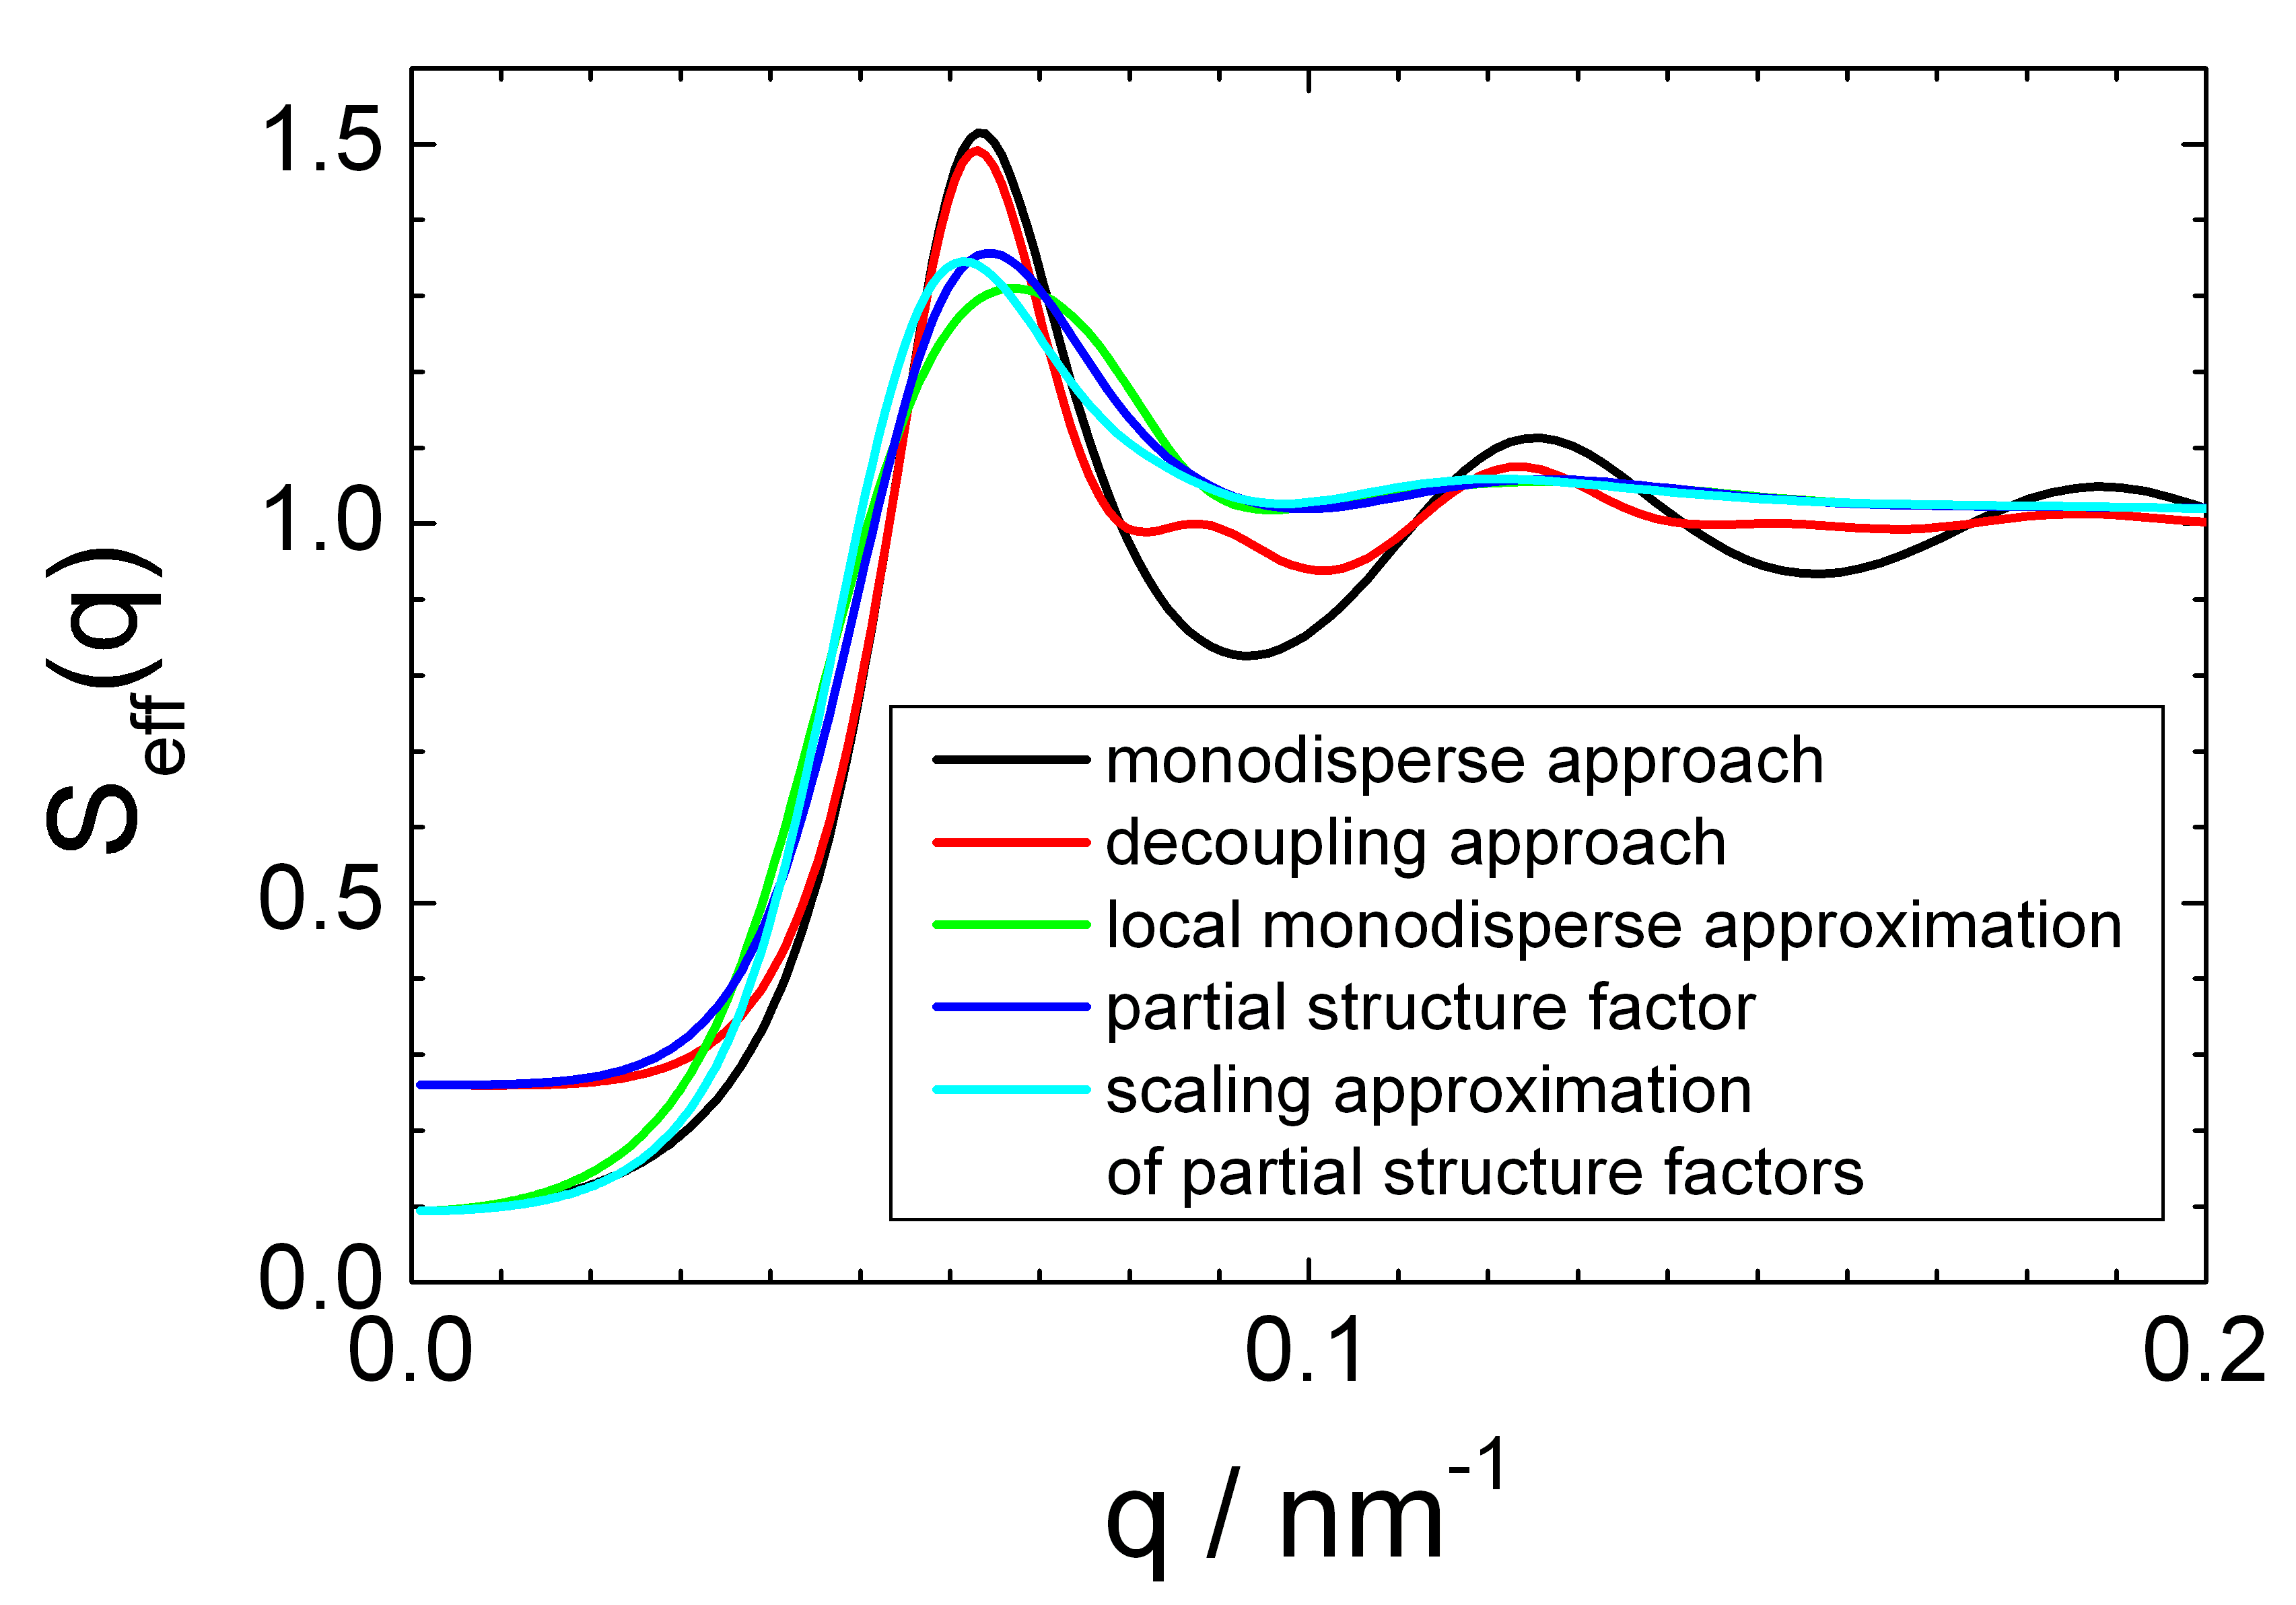
\includegraphics[width=0.65\textwidth,height=0.5\textwidth]{../images/structure_factor/Seff.png}
\end{center}
\caption{Effective structure factor $S_\text{eff}(q)$ for Spheres with Hard Sphere interaction potential.
The fraction is assumed to be $\eta=0.3$. A LogNormal distribution with $\sigma=0.15$ and $R_0=50nm$
is assumed.}
\label{fig:Seff}
\end{figure}

\clearpage
\section{Hard \& Sticky Hard Sphere}
\subsection{Hard Sphere \cite{Percus1958,Vrij1979}
}

\begin{equation}
U(r) =
 \begin{cases}
      \infty    & \text{for} \quad 0<r<\sigma \\
      0         & \text{for} \quad r>\sigma
   \end{cases}
\end{equation}

\begin{subequations}
\begin{align}
\alpha &= \frac{\left(1+2f_p\right)^2}{\left(1-f_p\right)^4} \\
\beta  &= -6 f_p \frac{\left(1 +f_p/2 \right)^2}{\left(1-f_p\right)^4} \\
\gamma &= \frac{f_p \alpha}{2}  \\
A &= 2 R_\text{HS} q
\end{align}

\begin{align}
G(q) =  & \, \alpha \, \frac{\sin A -A \cos A }{A^2} + \beta \, \frac{2 A \sin A +(2-A^2) \cos A -2}{A^3} + \nonumber \\
    & \, \gamma  \, \frac{-A^4 \cos A + 4\left[(3A^2-6)\cos A+(A^3-6A)\sin A+6\right]}{A^5}
\end{align}
\begin{align}
S_\text{HS}(q,R_\text{HS},f_p)  = & \cfrac{1}{1+24 f_p
\cfrac{G(f_p,R_\text{HS}q)}{R_\text{HS}q}}
\end{align}
\end{subequations}


\begin{figure}[htb]
\begin{center}
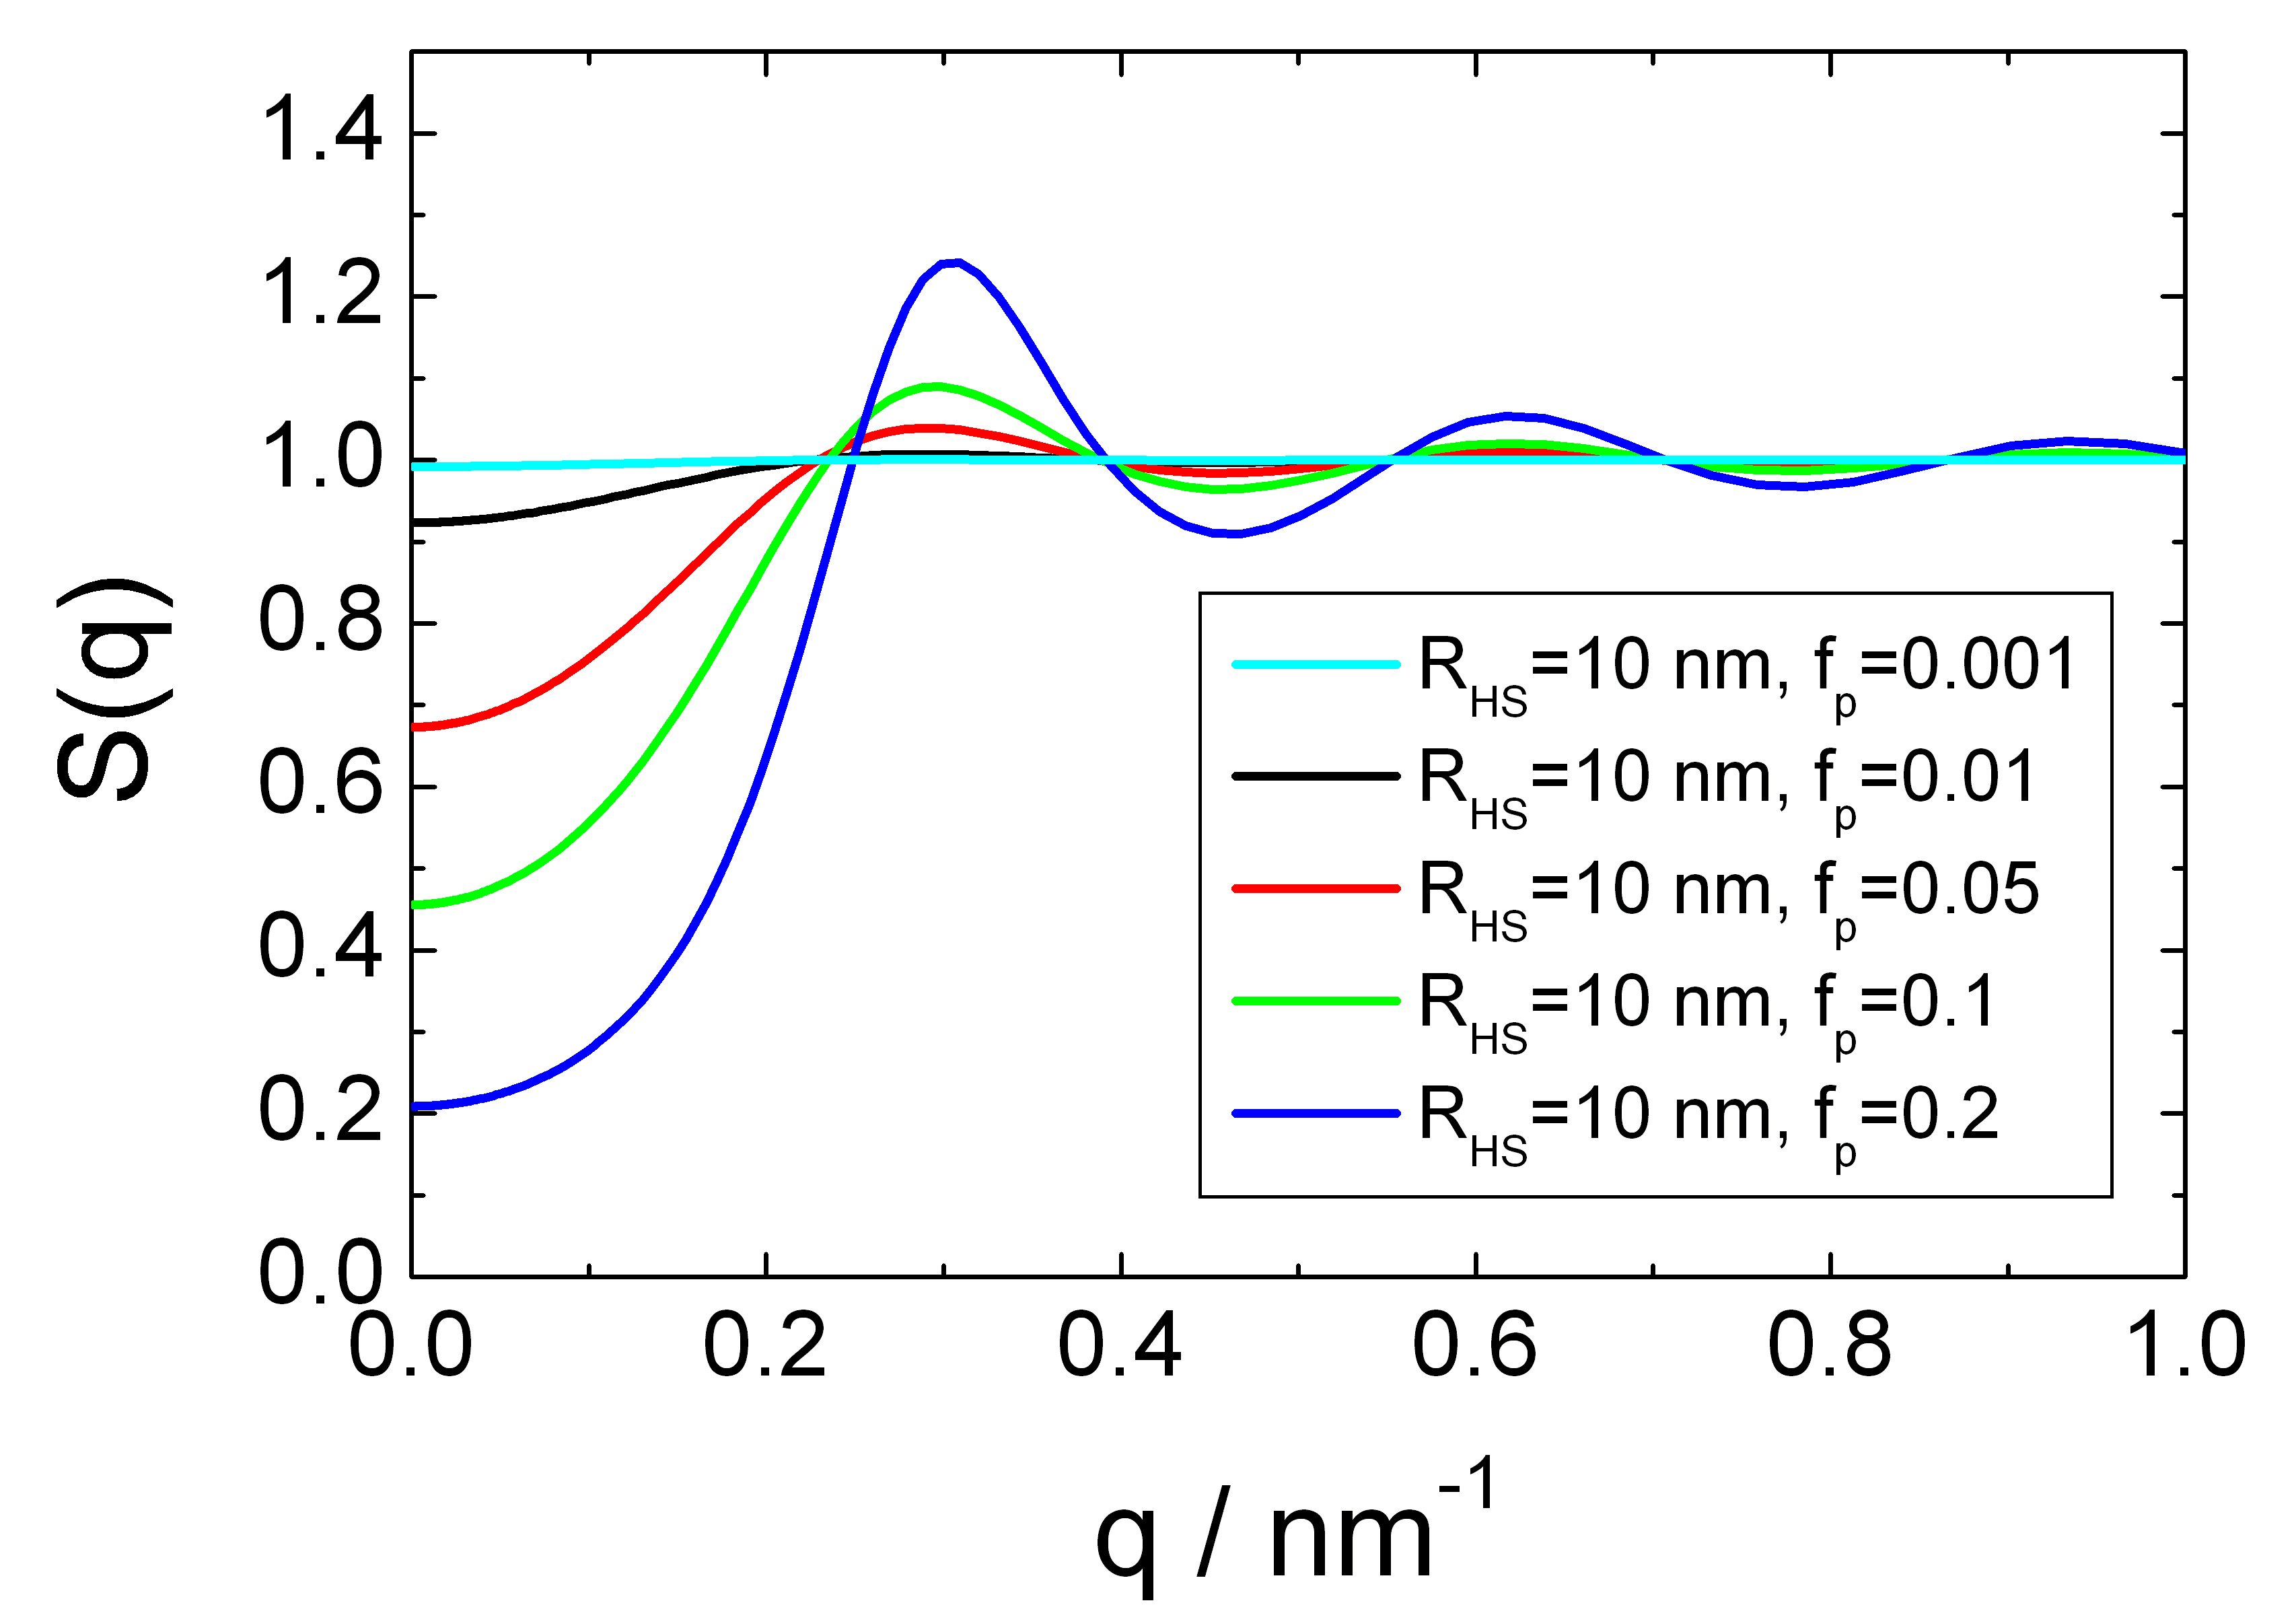
\includegraphics[width=0.768\textwidth,height=0.528\textwidth]{../images/structure_factor/HardSphere/HardSphereSQ.png}
\end{center}
\caption{Structure factor $S(q)$ for a hard sphere interaction potential for the different volume fractions $f_p$.}
\label{fig:SQHardSphere}
\end{figure}


%%%%%%%%%%%%%%%%%%%%%%%%%%%%%%%%%%%%%%%%%%%%%%%%%%%%%%%%%%%%%%%%%%%%%%%%%%%%%%%%%%%%%%

\clearpage
\subsection{Sticky Hard Sphere} ~\\

In Baxter's model \cite{Baxter1968,Robertus1989,Kruif1989,Barboy1974,Menon1991,Menon1991a}
of adhesive hard spheres the pair interaction potential $U(r)$ is replaces by
\begin{equation}
\frac{U(r)}{k_BT} =
 \begin{cases}
      \infty    & \text{for} \quad 0<r<\sigma \\
      \ln\frac{12\tau\Delta}{\sigma+\Delta} & \text{for} \quad \sigma<r<\sigma+\Delta \\
      0         & \text{for} \quad r>\sigma+\Delta
   \end{cases}
\end{equation}
after which, when applied, the limit $\Delta \to 0$ is taken.
Thus, only a single parameter, the so-called stickiness parameter
$\tau$, characterizes the adhesive strength.
\begin{subequations}
\begin{align}
\kappa &= 2 q R_\text{HS} \\
\eta &= f_p \left(\frac{2R_\text{HS}+\Delta}{2R_\text{HS}}\right)^3\\
\epsilon &= \tau+\frac{\eta}{1-\eta} \\
\gamma &= f_p\frac{1+\eta/2}{3\left(1-\eta\right)^2} \\
\lambda &= \frac{6}{\eta} \left(\epsilon-\sqrt{\epsilon^2-\gamma}\right)\\
\mu &= \lambda \eta (1-\eta) \\
\beta &= -\frac{3\eta \left(2+\eta\right)^2-2\mu \left(1+7\eta+\eta^2\right)+\mu^2(2+\eta)}{2\left(1-\eta\right)^4}\\
\alpha &= \frac{\left(1+2\eta-\mu\right)^2}{\left(1-\eta\right)^4}\\[5mm]
C(q) = & 2\frac{\eta\lambda}{\kappa}\sin\kappa
        -2\frac{\eta^2\lambda^2}{\kappa^2}\left(1-\cos\kappa\right) -\\
   \Big\{ & \alpha\kappa^3(\sin\kappa-\kappa\cos\kappa)
           +\beta\kappa^2(2\kappa\sin\kappa-(\kappa^2-2)\cos\kappa-2)\nonumber\\
          & +\frac{\eta\alpha}{2}\left((4\kappa^3-24\kappa)\sin\kappa-(\kappa^4-12\kappa^2+24)\cos\kappa+24\right)
             \Big\} \;\times\;24\frac{\eta}{\kappa^6}\nonumber
\end{align}
\begin{align}
   S_\text{sHS}(q,R_\text{HS},f_p,\tau) & = \frac{1}{1-C(q)}
\end{align}
\end{subequations}



\begin{figure}[htb]
\begin{center}
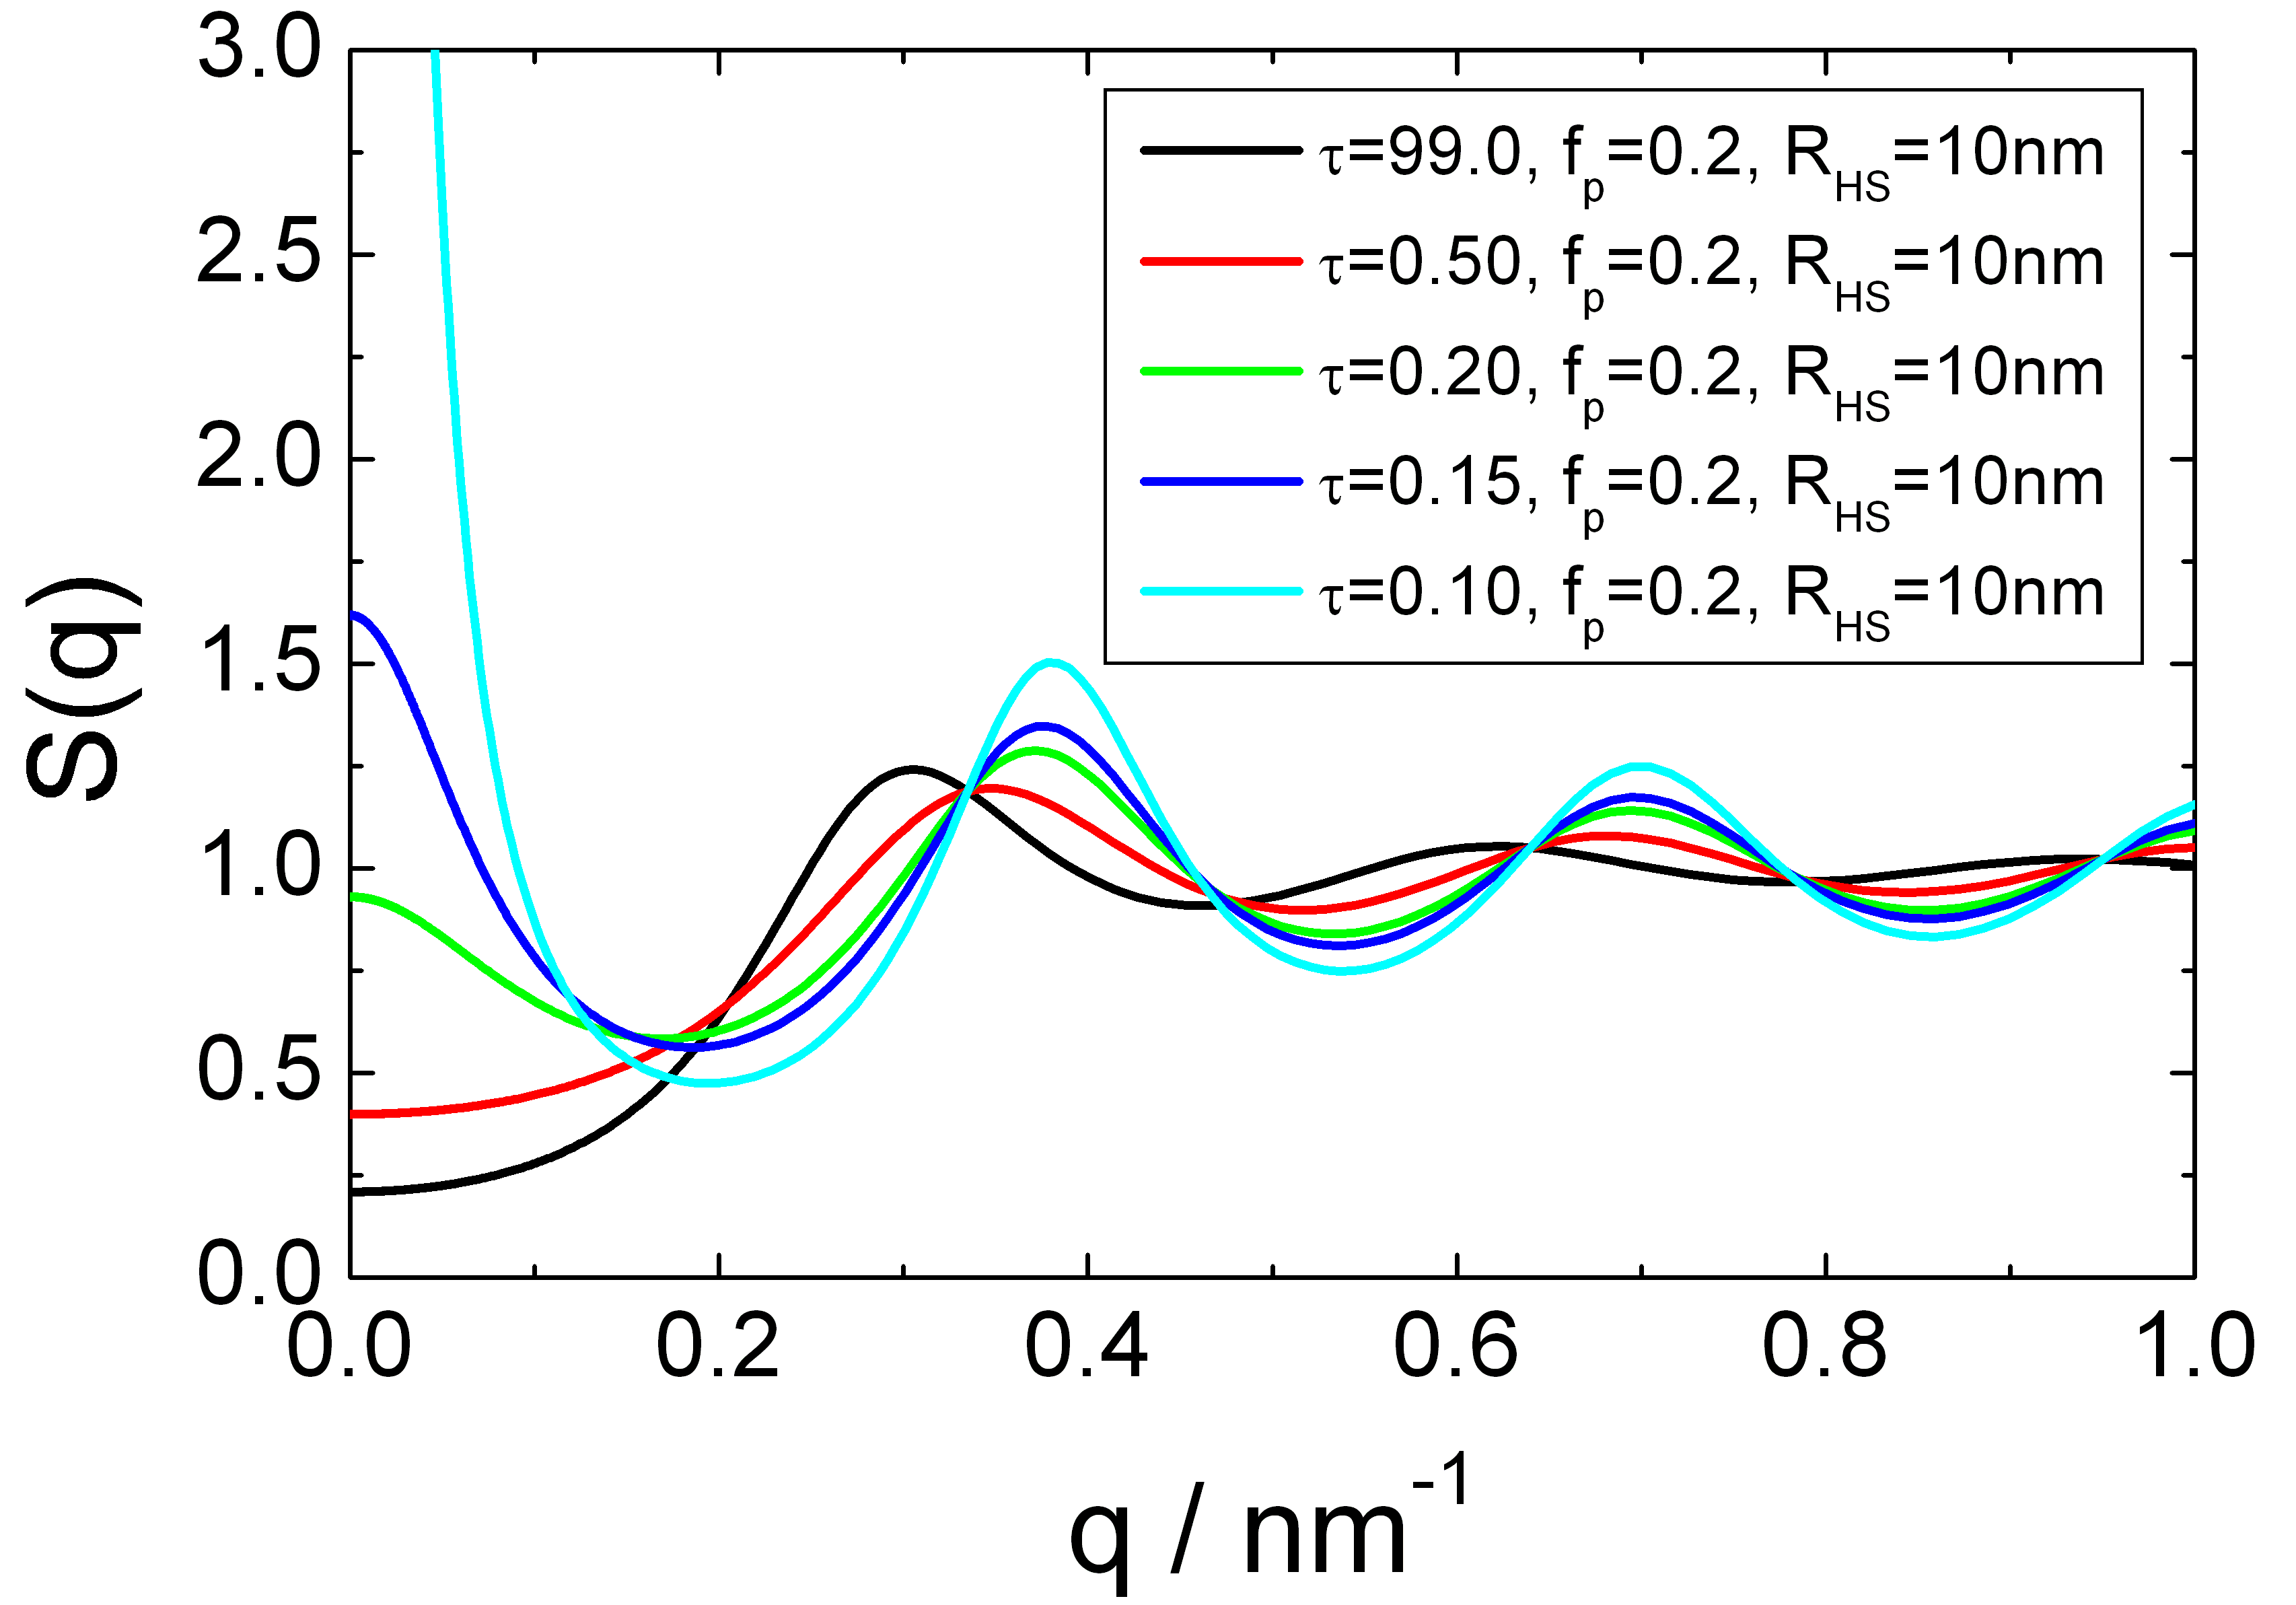
\includegraphics[width=0.768\textwidth,height=0.528\textwidth]{../images/structure_factor/HardSphere/StickyHardSphere1.png}
\end{center}
\caption{Structure factor $S(q)$ for a sticky hard sphere interaction potential for the different
stickiness parameters $\tau$.}
\label{fig:SQStickyHardSphere1}
\end{figure}
%%%%%%%%%%%%%%%%%%%%%%%%%%%%%%%%%%%%%%%%%%%%%%%%%%%%%%%%%%%%%%%%%%%%%%%%%%

\clearpage
\subsection{Sticky Hard Sphere ($2^\text{nd}$ version \cite{Regnaut1989,Regnaut1990})} ~\\

In Baxter's model of adhesive hard spheres the pair interaction
potential $U(r)$ is replaces by
\begin{equation}
\frac{U(r)}{k_BT} =
 \begin{cases}
      \infty    & \text{for} \quad 0<r<\sigma \\
      \ln\frac{12\tau\Delta}{\sigma+\Delta} & \text{for} \quad \sigma<r<\sigma+\Delta \\
      0         & \text{for} \quad r>\sigma+\Delta
   \end{cases}
\end{equation}



\begin{align}
\sigma &= 2R_\text{HS}+\Delta \\
\kappa & = q \sigma \\
\phi   &= f_p \left(\frac{\sigma}{2R_\text{HS}}\right)^3 \\
\lambda_{\pm} & =6 \left(\frac{\tau}{\phi}+\frac{1}{1-\phi}\right)
                \pm \sqrt{
                    36 \left[
                        \frac{\tau}{\phi}+\frac{1}{1-\phi}
                      \right]^2
                   -\frac{12}{\phi}\frac{1+\frac{\phi}{2}}{\left(1-\phi\right)^{2}}
                } \\
   \lambda & =
       \begin{cases}
           \lambda_+ & \mbox{for }\lambda_+ < \abs{\lambda_-} \\
           \lambda_- & \mbox{otherwise}
       \end{cases}
\\[5mm]
\mu & = \lambda \phi (1-\phi) \\
A & = \frac12 \; \frac{1+2 \phi-\mu}{\left(1-\phi\right)^2} \\
B & = \frac{\sigma}{2} \frac{\mu-3\phi}{2 \left(1-\phi\right)^2 } \\
C & = -A\sigma^2-B\sigma+\lambda\sigma^2/12 \\
I_n(\kappa) &= \int_0^1 x^n \cos(\kappa x)\; dx \\
J_n(\kappa) &= \int_0^1 x^n \sin(\kappa x)\; dx \\
\alpha & = 1-12 f_p \left( C\sigma^{-2}I_0(\kappa) + B\sigma^{-1} I_1(\kappa) +AI_2(\kappa) \right)\\
\beta  &=    12 f_p \left( C\sigma^{-2}J_0(\kappa) + B\sigma^{-1} J_1(\kappa) +AJ_2(\kappa) \right) \\
S(Q) & = \frac{1}{\alpha^2+\beta^2}
\end{align}


\begin{figure}[htb]
\begin{center}
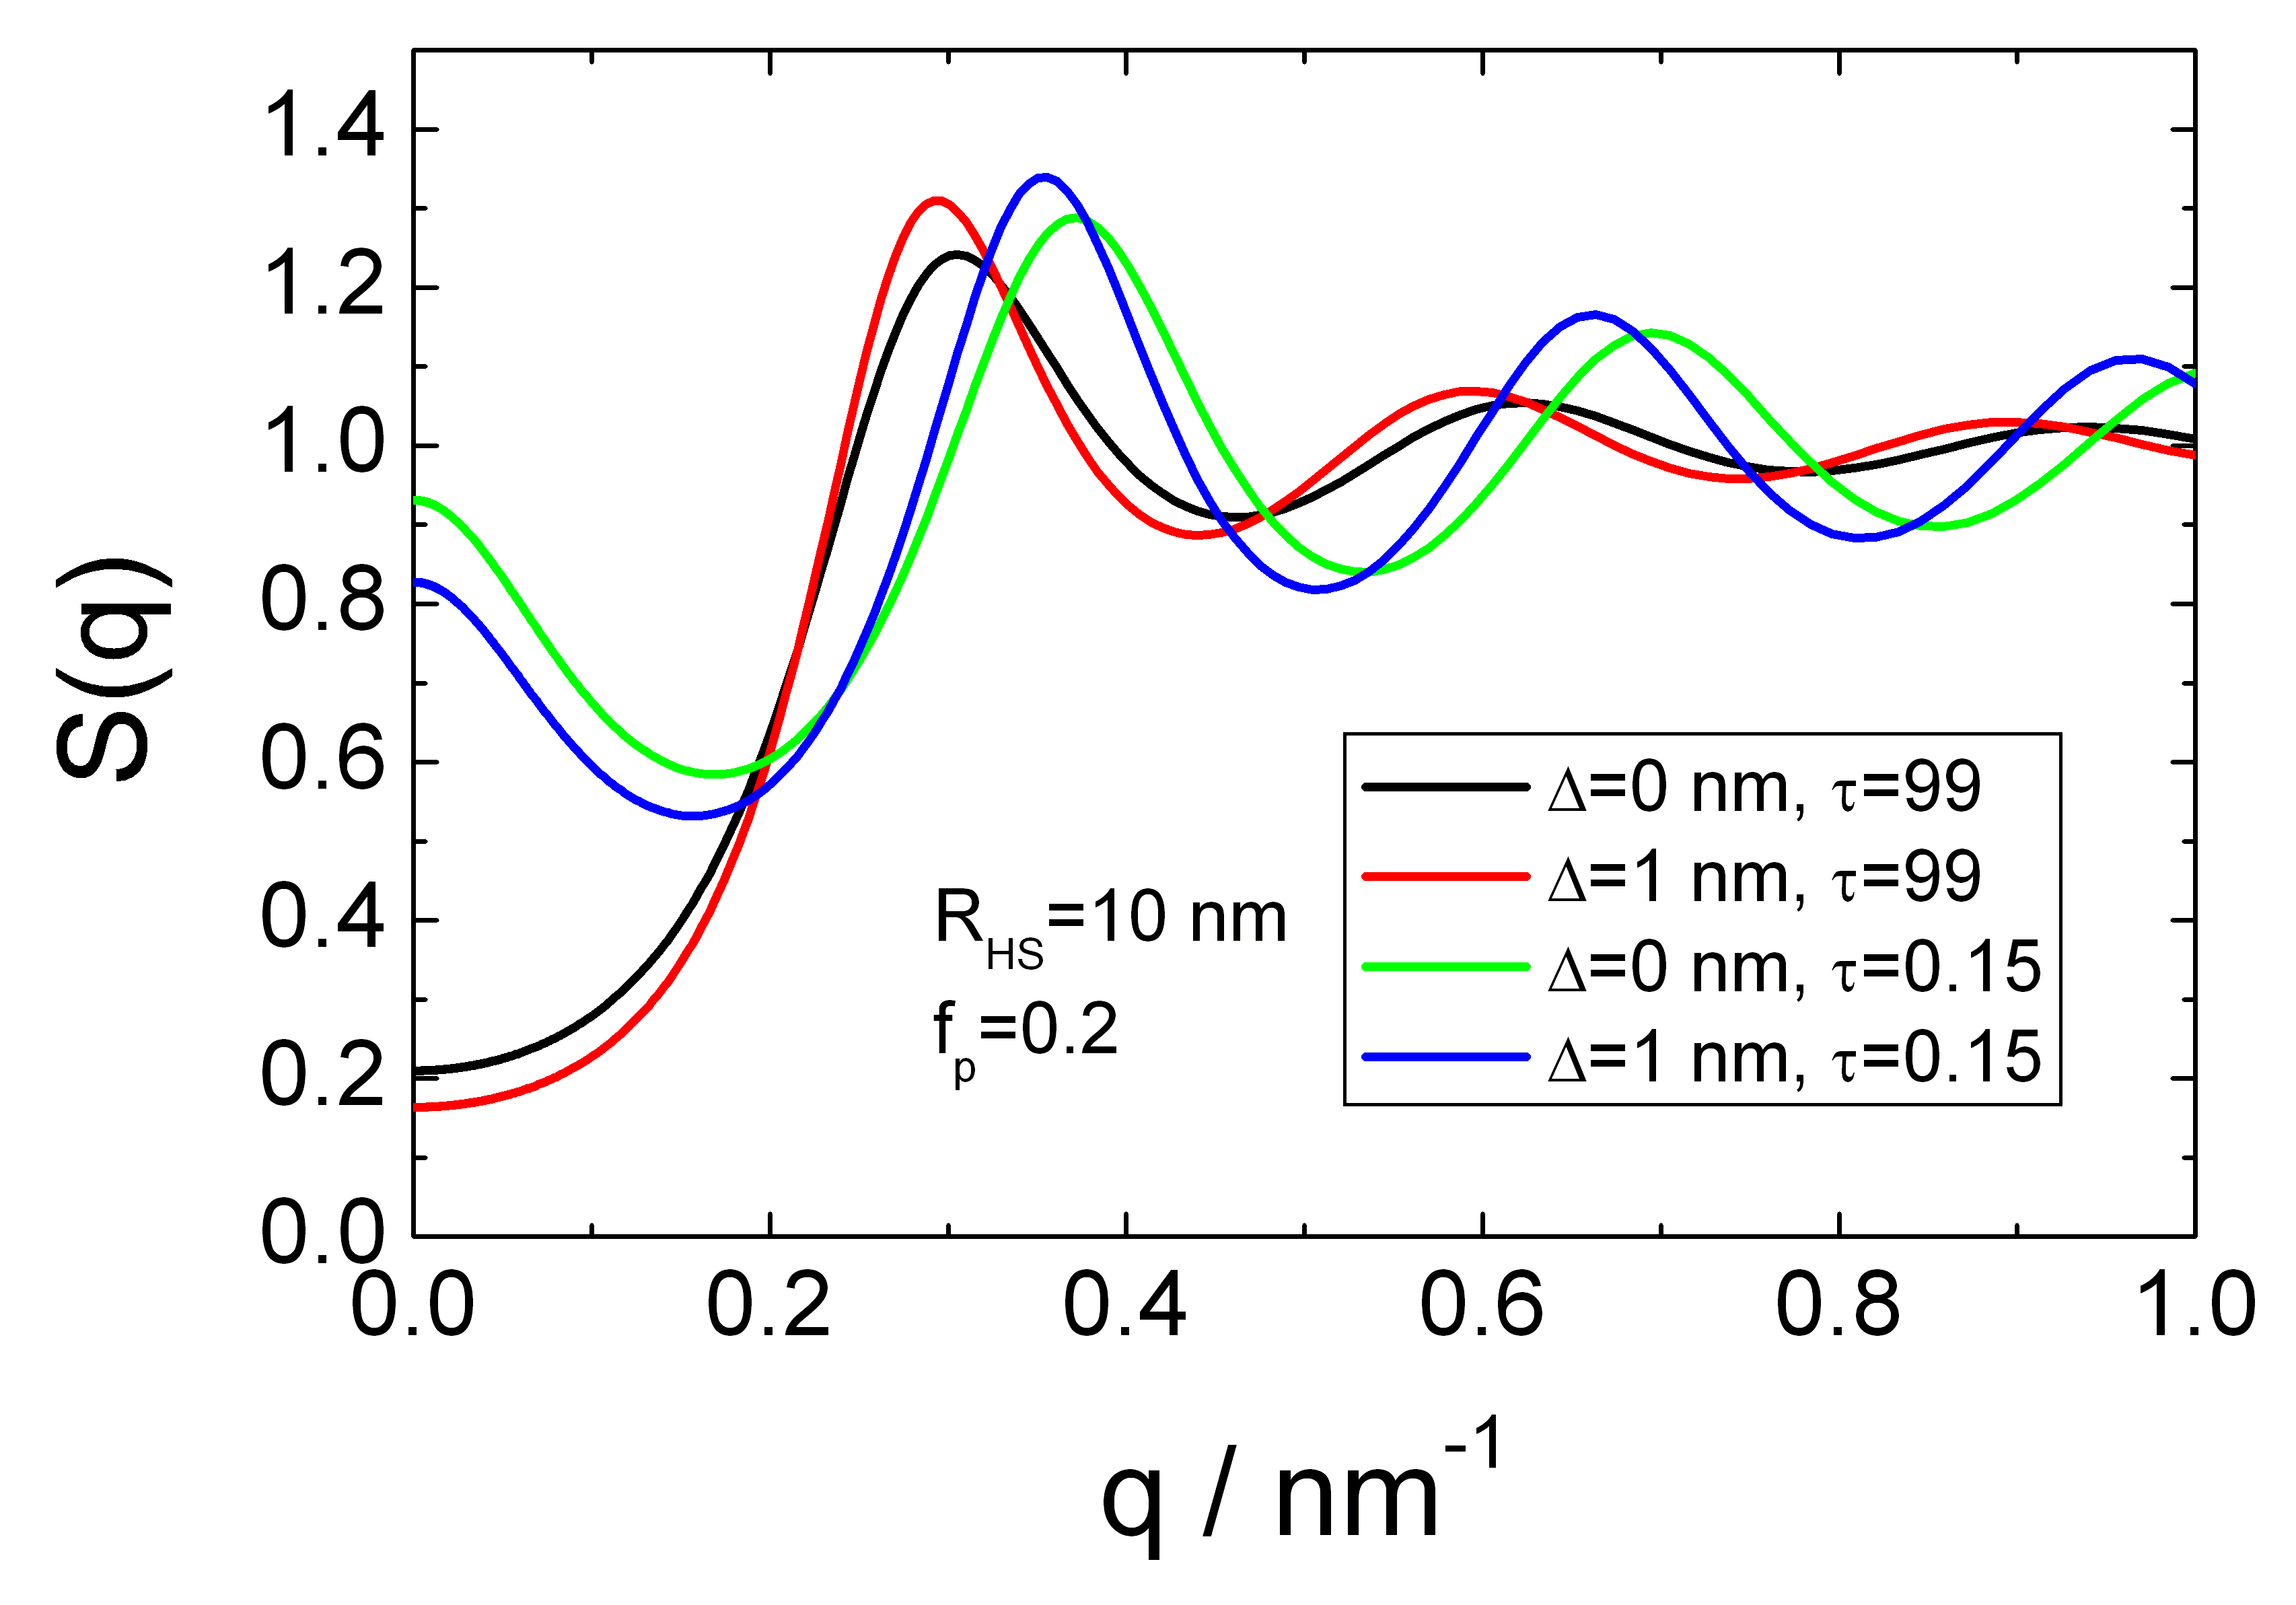
\includegraphics[width=0.768\textwidth,height=0.528\textwidth]{../images/structure_factor/HardSphere/StickyHardSphere2.png}
\end{center}
\caption{Structure factor $S(q)$ for a sticky hard sphere interaction potential for the different
stickiness parameters $\tau$.}
\label{fig:SQStickyHardSphere1}
\end{figure}

%%%%%%%%%%%%%%%%%%%%%%%%%%%%%%%%%%%%%%%%%%%%%%%%%%%%%%%%%%%%%%%%%%%%%%%%%%%%%%%%%%%%%

\clearpage
\subsection{Square Well Potential \cite{Sharma1977}} ~\\

The Square well potential can be written as
\begin{equation}
U(r) =
 \begin{cases}
      \infty    & \text{for} \quad 0<r<\sigma \\
      -\epsilon & \text{for} \quad \sigma<r<\lambda\sigma \\
      0         & \text{for} \quad r>\lambda\sigma
   \end{cases}
\end{equation}
where $\lambda$ and $\epsilon$ correspond to the breadth and the
depth of the square well potential. The structure factor $S(Q)$ is
than given by the following relations:
\begin{subequations}
\begin{align}
S(Q)  = & \frac{1}{1-C(Q)} \\
C(Q)  = & - \frac{24\eta}{(Q\sigma)^6} \Big\{ \alpha(Q\sigma)^3
\left[\sin(Q\sigma)-Q\sigma\cos(Q\sigma)\right] \\
        & +\beta(Q\sigma)^2\left[2Q\sigma\sin(Q\sigma)-(Q^2\sigma^2-2)\cos(Q\sigma)-2\right]\nonumber\\
        & +\gamma \left[(4Q^3\sigma^3-24Q\sigma)\sin(Q\sigma)-(Q^4\sigma^4-12Q^2\sigma^2+24)\cos(Q\sigma)+24\right] \nonumber\\
        & -\frac{\epsilon}{k_BT} (Q\sigma)^3\left[\sin(\lambda Q\sigma)-\lambda Q\sigma\cos(\lambda Q\sigma)+Q\sigma\cos(Q\sigma)-\sin(Q\sigma)\right]\Big\} \nonumber
\end{align}
where $\alpha$, $\beta$ and $\gamma$ are given by
\begin{align}
\alpha & = \frac{(1+2\eta)^2+\eta^3(\eta-4)}{(1-\eta)^4} \\
\beta  & = -\frac{1}{3}\eta\frac{18+20\eta-12\eta^2+\eta^4}{(1-\eta)^4} \\
\gamma & =
\frac{1}{2}\eta\frac{(1+2\eta)^2+\eta^3(\eta-4)}{(1-\eta)^4}
\end{align}
\end{subequations}
~\\
NOTE:\\
Values for the depth of $\epsilon>1.5k_BT$ and for the volume
fraction of $\eta> 0.08$ may give unphysical results when
compared to Monte Carlo simulations according to \cite{Sharma1977}.

\begin{figure}[htb]
\begin{center}
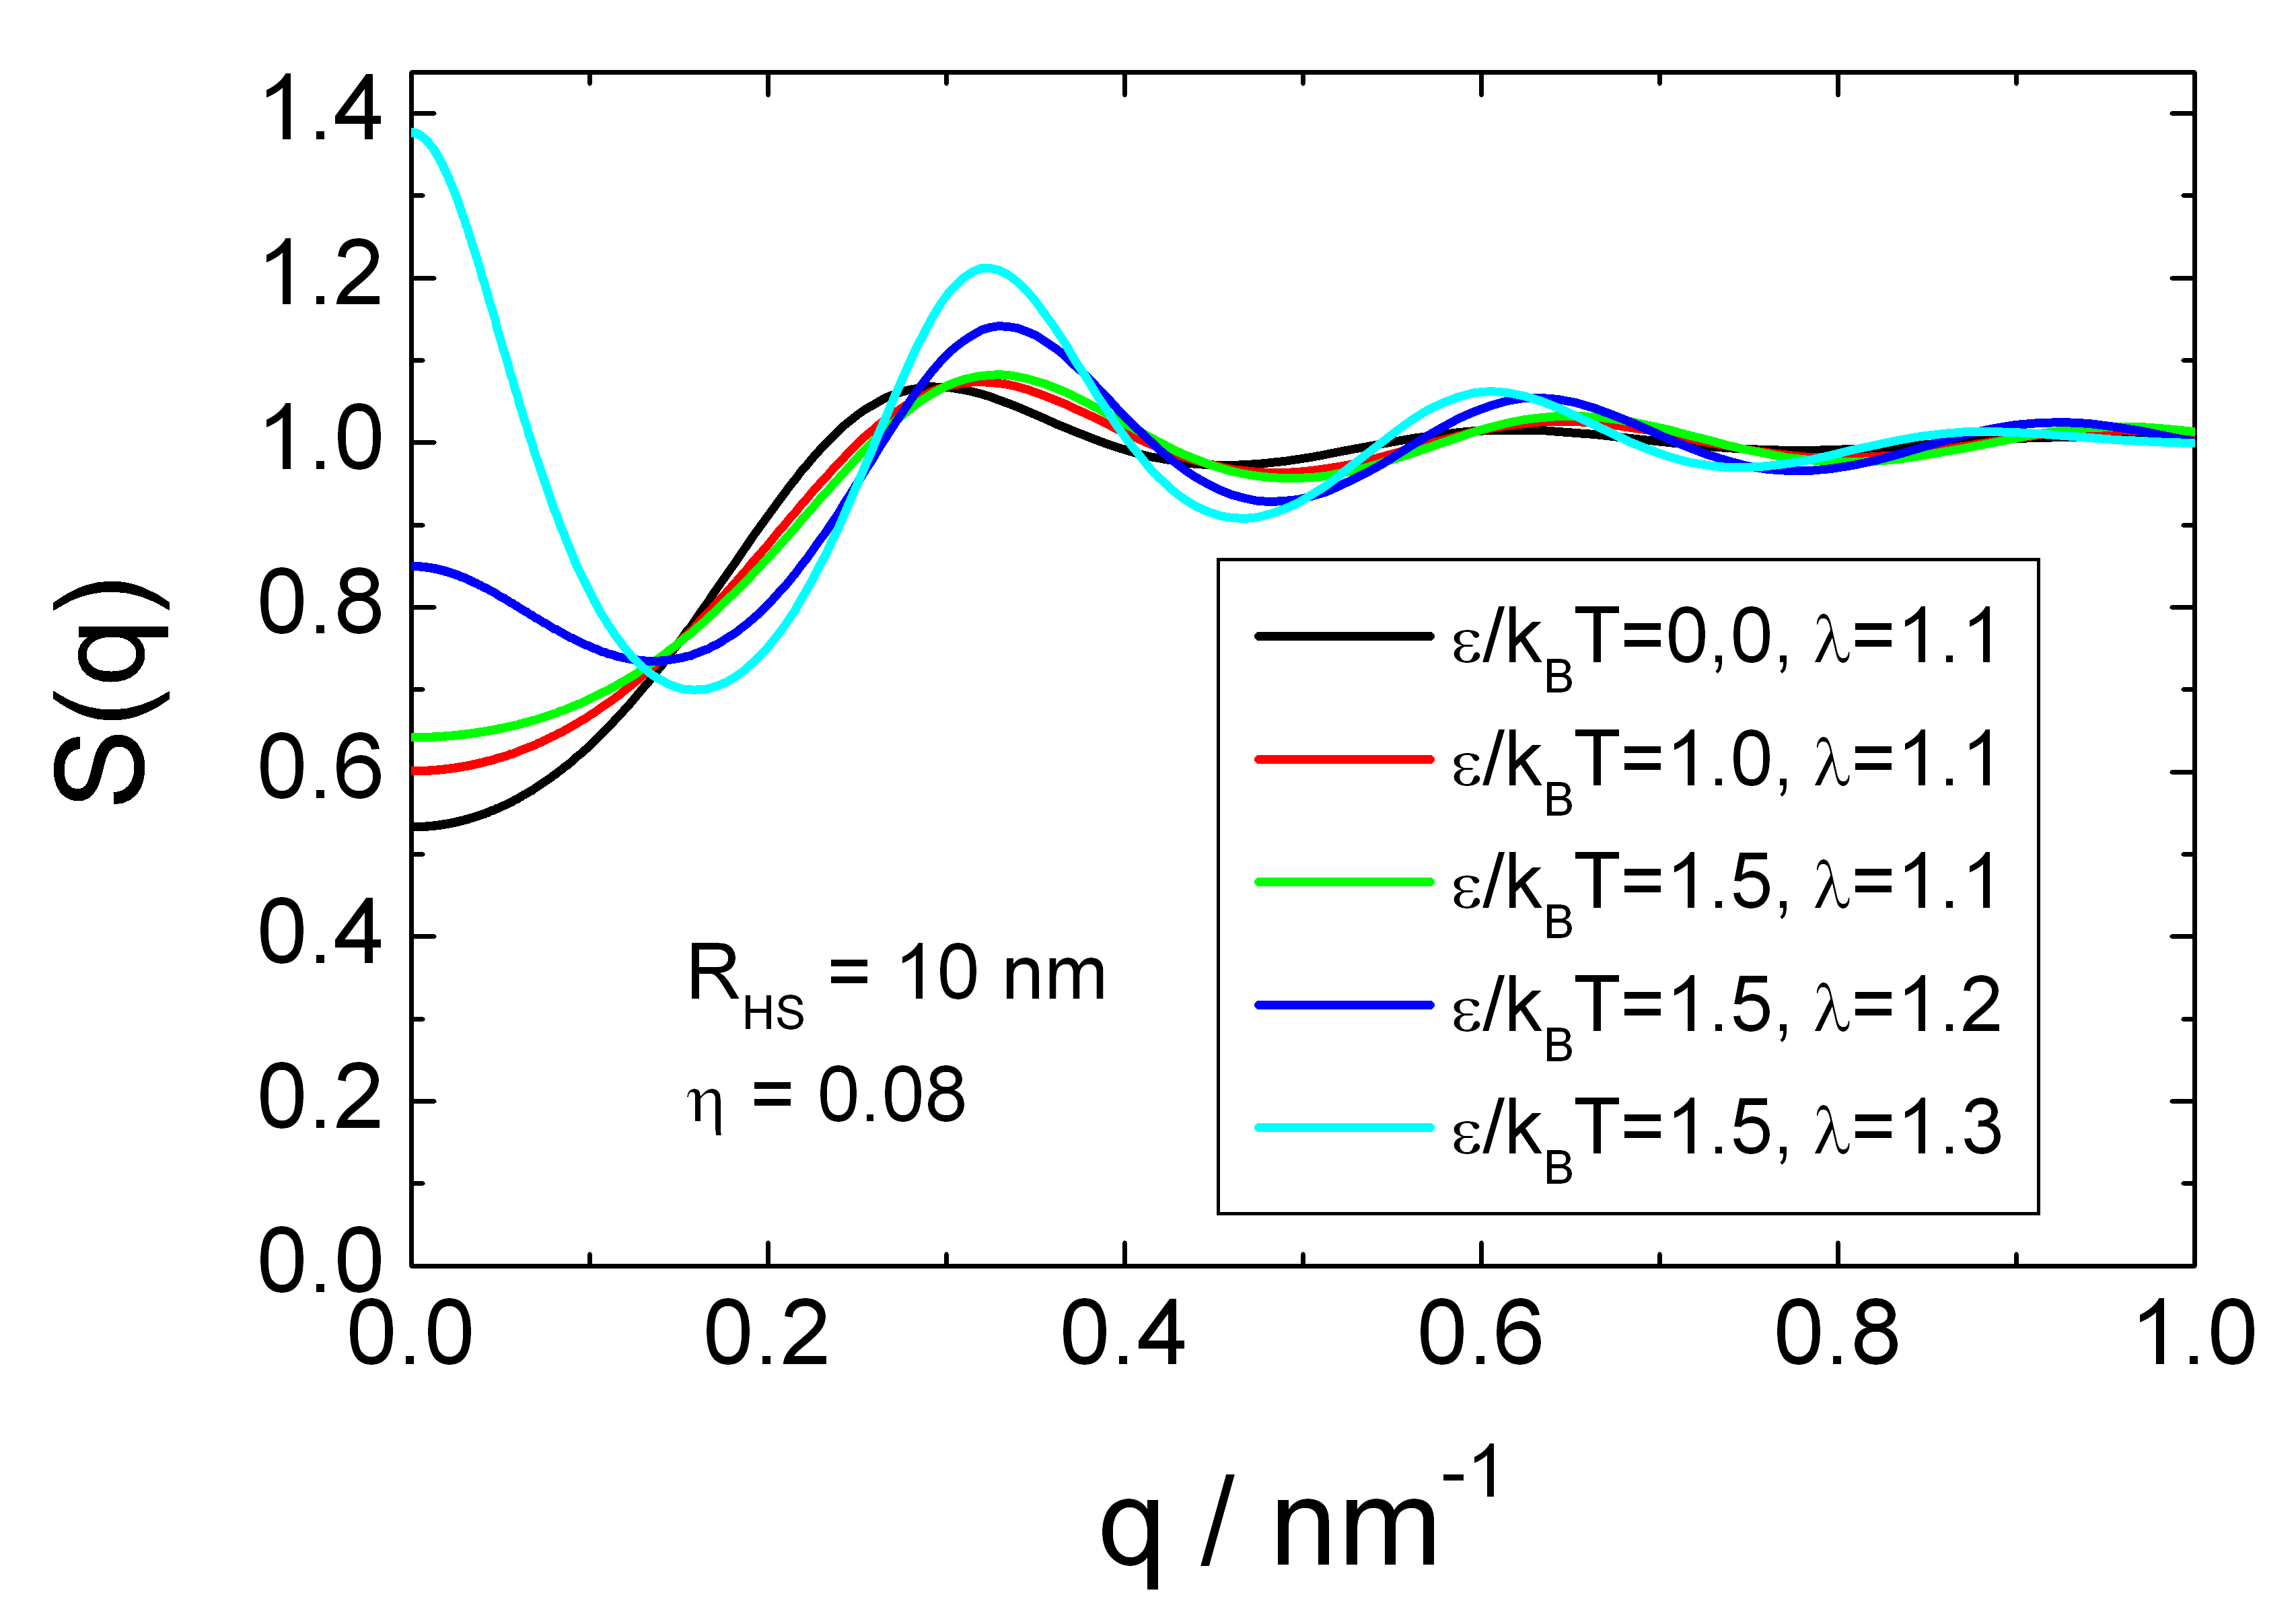
\includegraphics[width=0.768\textwidth,height=0.528\textwidth]{../images/structure_factor/HardSphere/SquareWellSQ.png}
\end{center}
\caption{Structure factor $S(q)$ for a square well interaction potential.}
\label{fig:SquareWell1}
\end{figure}

%%%%%%%%%%%%%%%%%%%%%%%%%%%%%%%%%%%%%%%%%%%%%%%%%%%%%%%%%%%%%%%%%%%%%%%%%%%%%%%%%%

\clearpage
\subsection{Square Well Potential 2} ~\\

The Square well potential can be written as
\begin{equation}
U(r) =
 \begin{cases}
      \infty    & \text{for} \quad 0<r<\sigma \\
      -\epsilon & \text{for} \quad \sigma<r<\sigma+\Delta \\
      0         & \text{for} \quad r>\sigma+\Delta
   \end{cases}
\end{equation}
where $\Delta$ and $\epsilon$ correspond to the width and the
depth of the square well potential. The structure factor $S(Q)$ is
than given by the following relations:
\begin{equation}
S(Q)  = 1
-4\pi\rho\sigma^3\frac{\sin(Q\sigma)-Q\sigma\cos(Q\sigma)}{Q^3\sigma^3}
          +4\pi\rho\sigma^2\left[e^{\frac{\epsilon}{k_BT}}-1\right]\frac{\sin(Q\sigma)}{Q\sigma}
          \Delta
\end{equation}
where $\sigma$ is the particle diameter ($R_{HS} = \sigma/2$: hard
sphere radius is requested by software as input parameter),
$\Delta$ the width of the square well potential, $\epsilon$ (input
value in software is $\epsilon/k_B$, i.e. in Kelvin), $T$ (in
Kelvin) the sample temperature, the depth and $\rho$ the colloid
concentration, which is related to the colloid volume fraction
$\eta$ by $\eta=\pi\rho\sigma^3/6$.


%%%%%%%%%%%%%%%%%%%%%%%%%%%%%%%%%%%%%%%%%%%%%%%%%%%%%%%%%%%%%%%%%%%%%%

\clearpage
\section{Multi Lamellar Structures \cite{Pabst2003,Fruhwirth2004}}
\subsection{Multi-Lamellar Structures, Thermal Disorder} \hspace{1pt}\\

\begin{figure}[htb]
\begin{center}
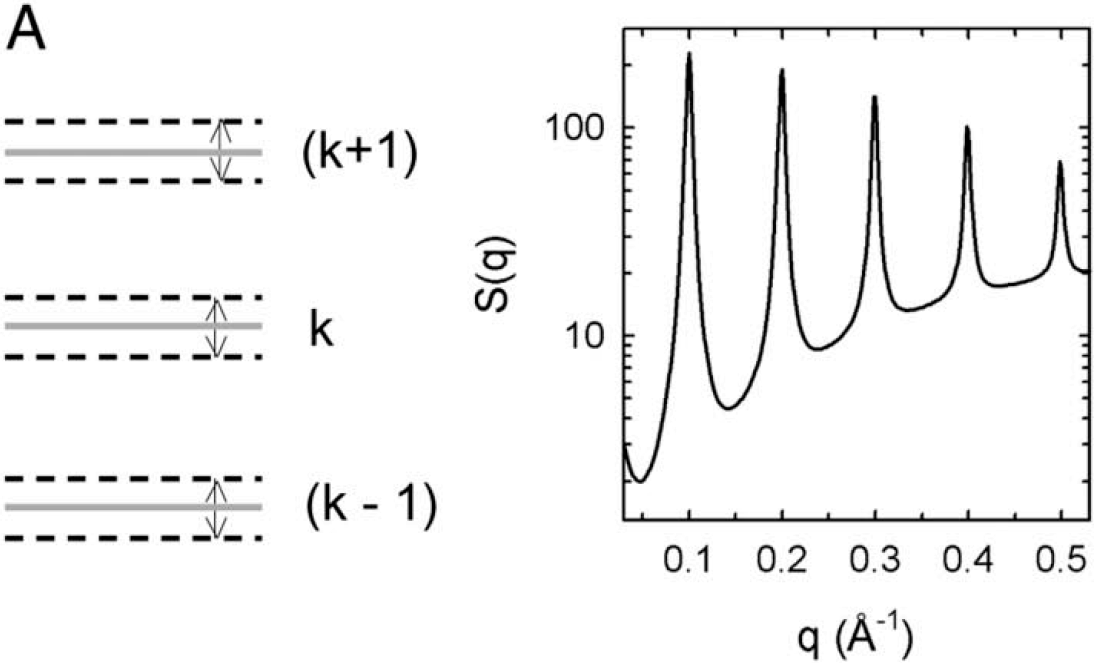
\includegraphics[width=0.7\textwidth,height=0.4\textwidth]{ThermalDisorderSQ.png}
\end{center}
\caption{Thermal disorder, considering fluctuations of flat layers
around well defined and evenly spaced equilibrium positions.}
\label{ThermalDisorderSQ}
\end{figure}

The first type describes thermal disorder (TD) caused by small
fluctuations of the bilayers around well defined mean layer
positions of equal separation (Fig. \ref{ThermalDisorderSQ}). In
such a crystal lattice the long-range order is preserved and the
structure factor for a single domain of size $L = Nd$ is identical
to that of a perfect finite crystal multiplied by the well known
Debye-Waller temperature factor, where $\Delta = \left<
(d_k-d)^2\right>$ denotes the mean square fluctuations of the
bilayers. As shown in Fig. \ref{ThermalDisorderSQ},
$S_\text{TD}(Q)$ is characterized by a set of Bragg peaks of equal
width, the diffraction order amplitudes of which decrease
exponentially with the Debye-Waller factor. The lost intensity is
found as a diffuse background scattering, which increases to the
limit of $N$ for large $Q$.
\begin{align}
S_\text{TD}(Q,N,d,\Delta,N_\text{diff}) = N_\text{diff} + \sum_{N_k=N-2\sigma}^{N+2\sigma} x_k
S_\text{k,TD}
\end{align}
with
\begin{align}
S_\text{k,TD} & = \left( N_k + 2 \exp\left(
-\frac{Q^2\Delta^2}{2}\right) \sum_{m=1}^{N_k-1} (N_k-m) \cos(mQd)
\right)
\end{align}
$N_\text{diff}$ accounts for an additional
diffuse background, due to a number of uncorrelated
scattering bilayers in $S_\text{TD}(Q,N,d,\Delta,N_\text{diff})$,
which is not included in the TD theory.
Its origin is attributed to bilayers with strong lattice defects or
unilamellar vesicles, which display neither short-range nor
(quasi-) long-range order.

The structure factors $S_\text{k,TD}(Q)$ with low, but fixed
stacking numbers $N$ show oscillations at low $Q$ (as can be seen in
Fig. \ref{ThermalDisorderSQ}), but no such oscillations are found in
experimental data. This can be understood as the consequence of
polydispersity in the size of the different stacks. In order to
eliminate these artifacts from strictly monodisperse systems, we use
a `polydisperse' structure factor, i.e. we use an average of a
series of structure factors with varying numbers of bilayers
\cite{Fruhwirth2004}. The analytical form of the distribution is not
known a priori. We use a Gaussian distribution approximated by a
discrete series The standard deviation $\sigma$ for the
Gaussian-weighted distribution is chosen as
\begin{align}
\sigma =
\begin{cases}
\sqrt{N} & \text{for} N\geq 5 \text{,} \\
0.5(N-1) & \text{for} N< 5
\end{cases}
\end{align}
Therefore, $N$ must be greater or equal to 2, which is a
reasonable restriction for multilamellar stacks of bilayers. In
the range of $N \pm 2\sigma$, structure factors weighted by
\begin{align}
x_k & = \frac{1}{\sigma\sqrt{2\pi}} \exp\left[
-\frac{(N_k-N)^2}{2\sigma^2}\right]
\end{align}
are calculated, where $N$ is the mean number of stacks and $N_k$
is one of the  bilayers in the range $N\pm 2\sigma$. This
polydispersity model does not introduce new free parameters and is
symmetrical around the mean $N$.

\begin{figure}[htb]
\begin{center}
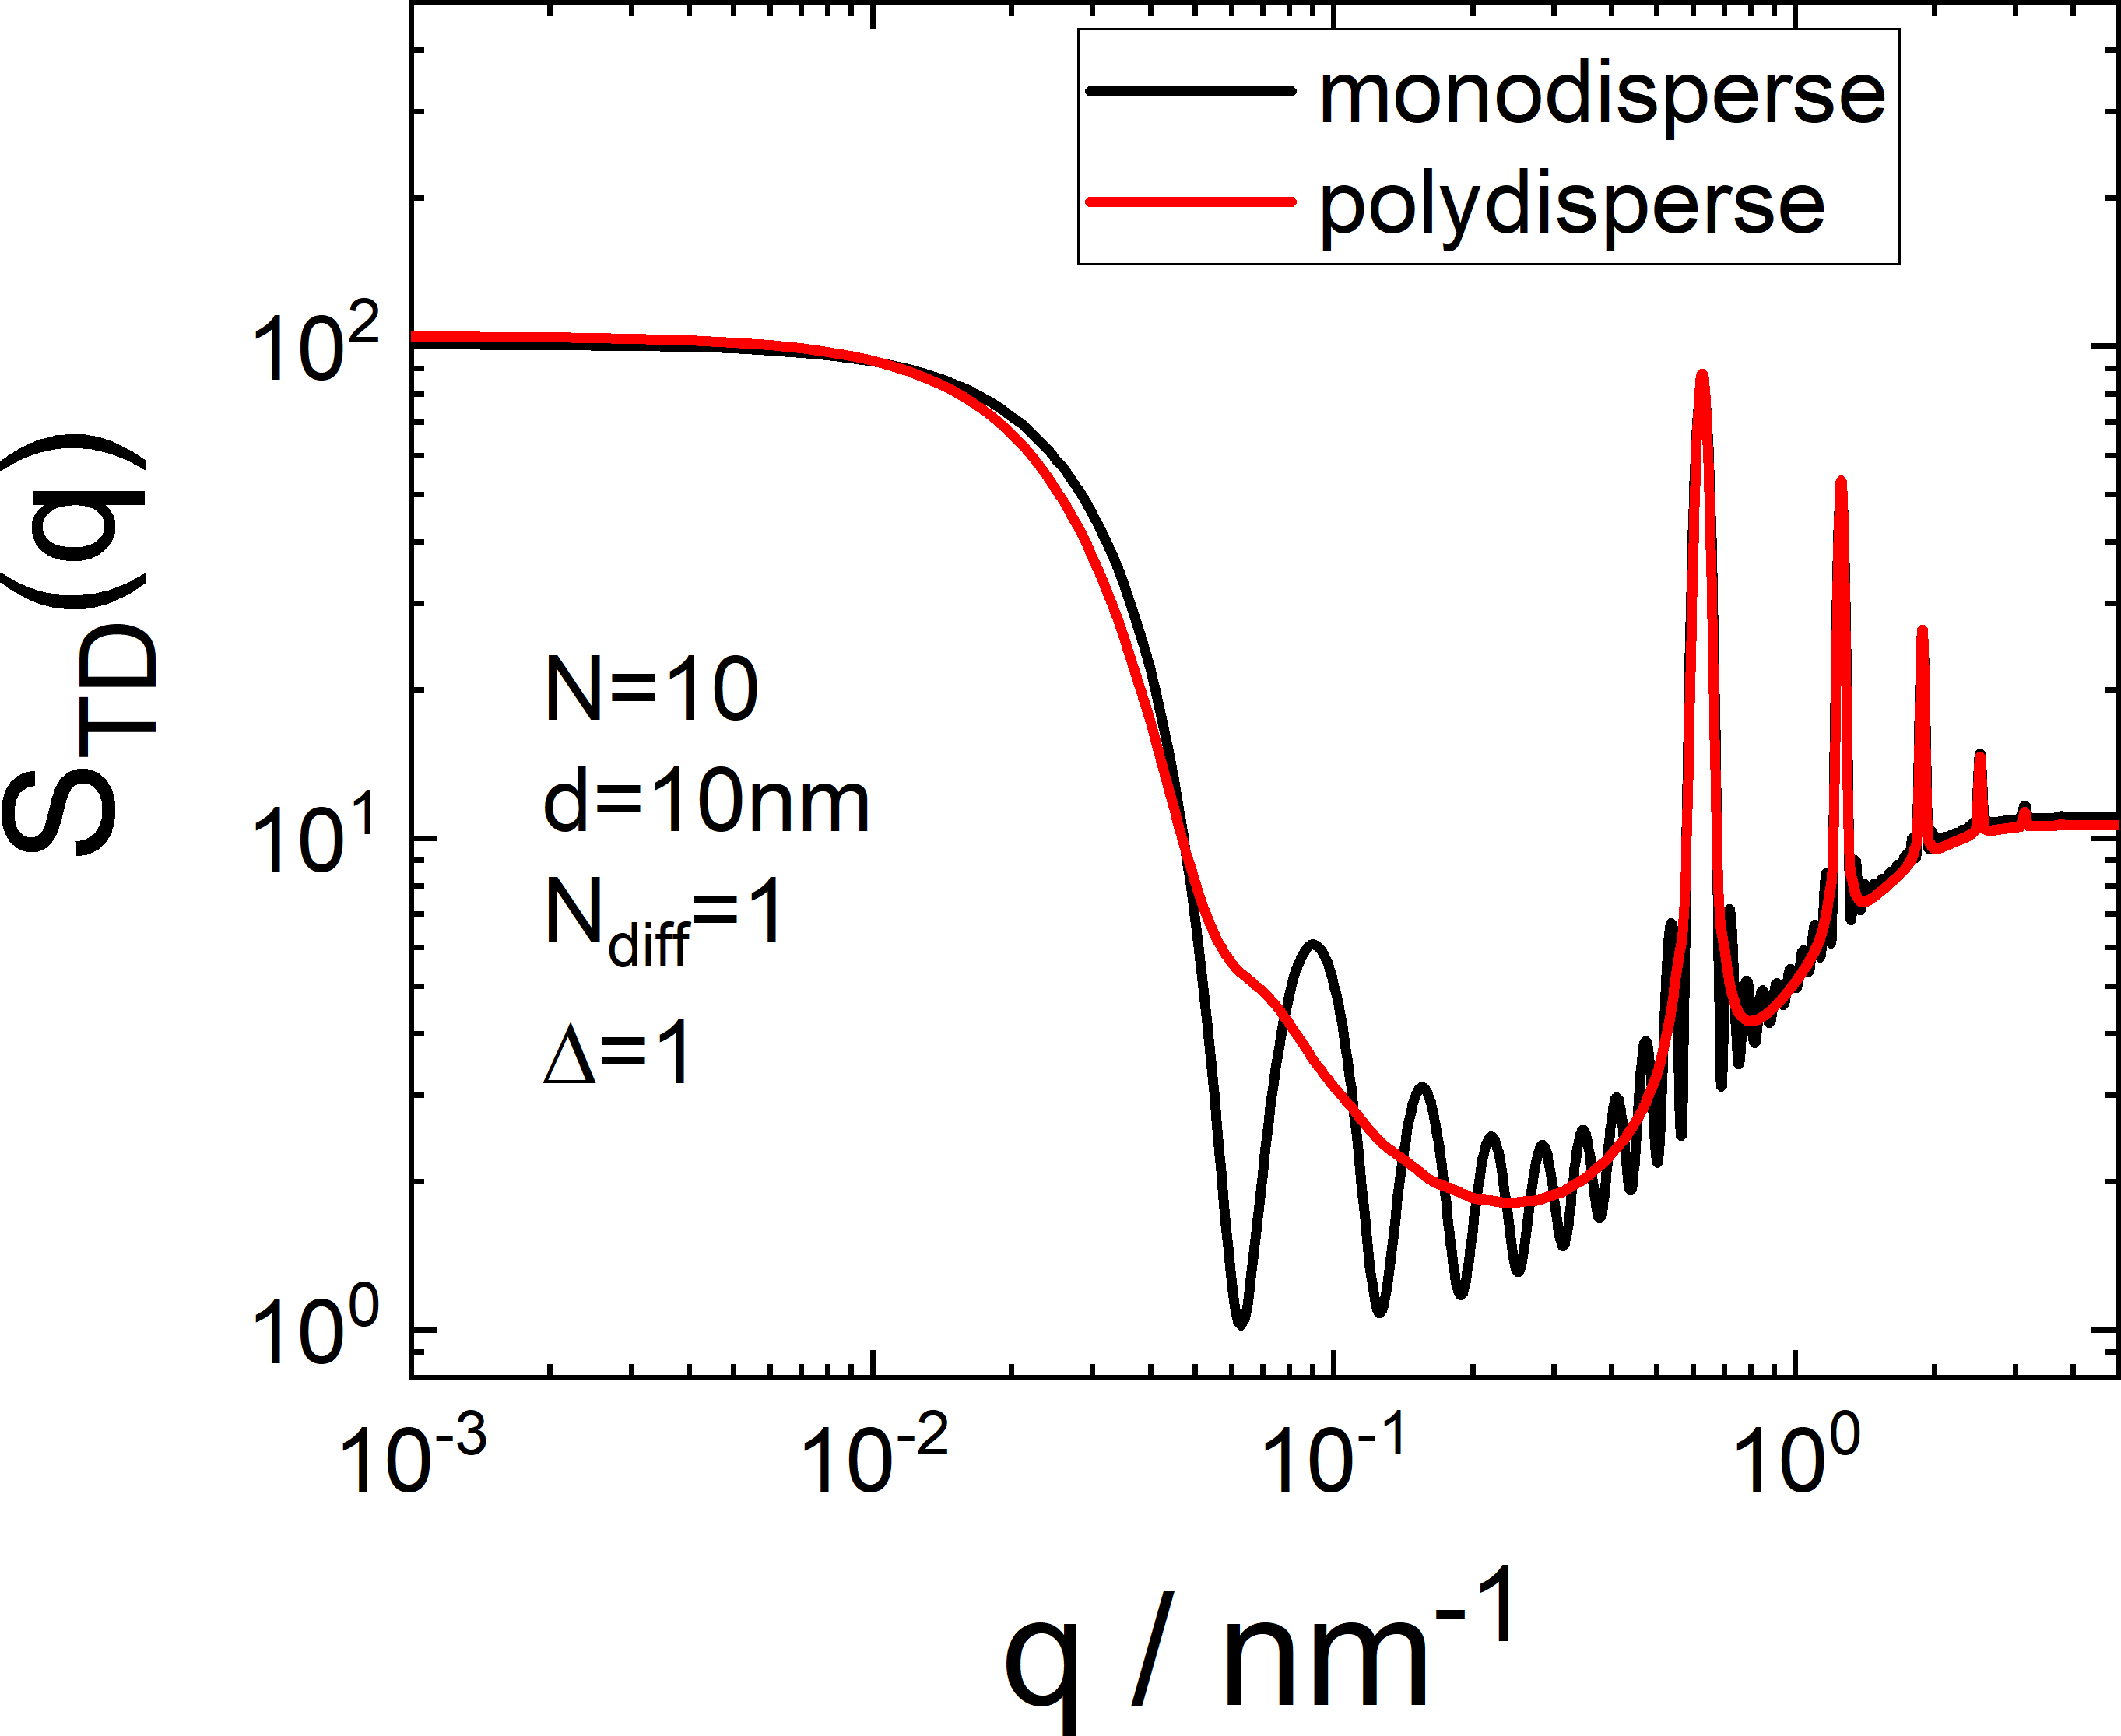
\includegraphics[width=0.65\textwidth,height=0.5\textwidth]{../images/structure_factor/Lamellar/TDLamellar.png}
\end{center}
\caption{Structure factor of multi-lamellar structures with thermal disorder. }
\label{fig:TDLamellar}
\end{figure}

\vspace{5mm}

\noindent
\underline{Input Parameters for model \texttt{ThermalDisorder}:}
\begin{description}
\item[\texttt{N}] mean number of stacks $N$
\item[\texttt{d}] stacking separation $d$
\item[\texttt{Delta}]  Debye-Waller disorder parameter $\Delta$
\item[\texttt{Nu}]   number of uncorrelated scattering bilayers $N_\text{diff}$
\end{description}

\noindent\underline{Note:}
\begin{itemize}
\item This structure factor is intended to be used with the \texttt{monodisperse approximation}.
\end{itemize}

%%%%%%%%%%%%%%%%%%%%%%%%%%%%%%%%%%%%%%%%%%%%%%%%%%%%%%%%%%%%%%%%%%%%%%%%%%%%%%%%%%%%%%%%%%

\clearpage
\subsection{Multi-Lamellar Structures, Paracrystalline Theory} ~\\

\begin{figure}[htb]
\begin{center}
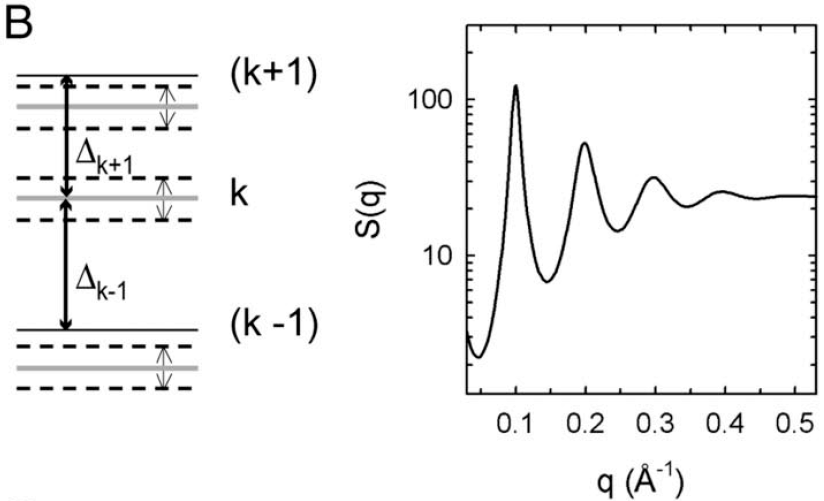
\includegraphics[width=0.7\textwidth,height=0.4\textwidth]{ParacrystallineTheorySQ.png}
\end{center}
\caption{Stacking disorder as described within paracrystalline
theory (PT) is due to displacements from the mean layer
positions.} \label{ParacrystallineTheorySQ}
\end{figure}


The second type of disorder accounts for the presence of small
variations in the bilayer separations (Fig.
\ref{ParacrystallineTheorySQ}), so-called stacking disorder, and is
described within the paracrystalline theory (PT)
\cite{Hosemann1962,Guinier1963,Blaurock1982}. As the position of an
individual fluctuating layer in a paracrystal is determined solely
by its nearestneighbour membranes, the crystalline long-range order
is lost. Still, we are able to observe Bragg-peak scattering due to
the fact that there is quasi long-range order. However, these
quasi-Bragg peaks will display a typical line shape. In the case of
disorder of the second kind, the structure factor derived from
paracrystalline theory is given by \cite{Guinier1963}
\begin{align}
S_\text{PT}(Q,N,d,\Delta,N_\text{diff}+) = N_\text{diff}+\sum_{N_k=N-2\sigma}^{N+2\sigma} x_k
S_\text{k,PT}
\end{align}
with
\begin{align}
S_\text{k,PT} &= \left( N_k + 2 \sum_{m=1}^{N_k-1} (N_k-m)
\cos(mQd) \exp\left( -\frac{m^2Q^2\Delta^2}{2}\right) \right)
\end{align}
$N_\text{diff}$ accounts for an additional
diffuse background, due to a number of uncorrelated
scattering bilayers in $S_\text{PT}(Q,N,d,\Delta,N_\text{diff})$,
which is not included in the paracrystalline theory.
Its origin is attributed to bilayers with strong lattice defects or
unilamellar vesicles, which display neither short-range nor
(quasi-) long-range order.

Fig. \ref{ParacrystallineTheorySQ} shows that the quasi-Bragg peak
intensity decreases for $S_\text{PT}(Q)$, as in the previous case of
thermal disorder. However, the decrease in peak height is also
accompanied by a progressive broadening proportional to the square
of the diffraction order $h$ \cite{Schwartz1975}. The line shape of
the tails is essentially Lorentzian with
$$S_\text{k,PT}(Q) \propto (Q - Q_h)^2,$$
where $Q_h$ is the position of the $h^\text{th}$ diffraction order
in $Q$ space. Again, the loss in intensity shows up as diffuse
background scattering, which is stronger than from pure thermal
disorder.


The structure factors $S_\text{k,PT}(Q)$ with low, but fixed
stacking numbers $N$ show oscillations at low $Q$ (as can be seen in
Fig. \ref{ParacrystallineTheorySQ}), but no such oscillations are
found in experimental data. This can be understood as the
consequence of polydispersity in the size of the different stacks.
In order to eliminate these artifacts from strictly monodisperse
systems, we use a `polydisperse' structure factor, i.e. we use an
average of a series of structure factors with varying numbers of
bilayers \cite{Fruhwirth2004}. The analytical form of the
distribution is not known a priori. We use a Gaussian distribution
approximated by a discrete series The standard deviation $\sigma$
for the Gaussian-weighted distribution is chosen as
\begin{align}
\sigma =
\begin{cases}
\sqrt{N} & \text{for} N\geq 5 \text{,} \\
0.5(N-1) & \text{for} N< 5
\end{cases}
\end{align}
Therefore, $N$ must be greater or equal to 2, which is a
reasonable restriction for multilamellar stacks of bilayers. In
the range of $N \pm 2\sigma$, structure factors weighted by
\begin{align}
x_k & = \frac{1}{\sigma\sqrt{2\pi}} \exp\left[
-\frac{(N_k-N)^2}{2\sigma^2}\right]
\end{align}
are calculated, where $N$ is the mean number of stacks and $N_k$
is one of the  bilayers in the range $N\pm 2\sigma$. This
polydispersity model does not introduce new free parameters and is
symmetrical around the mean $N$.


\begin{figure}[htb]
\begin{center}
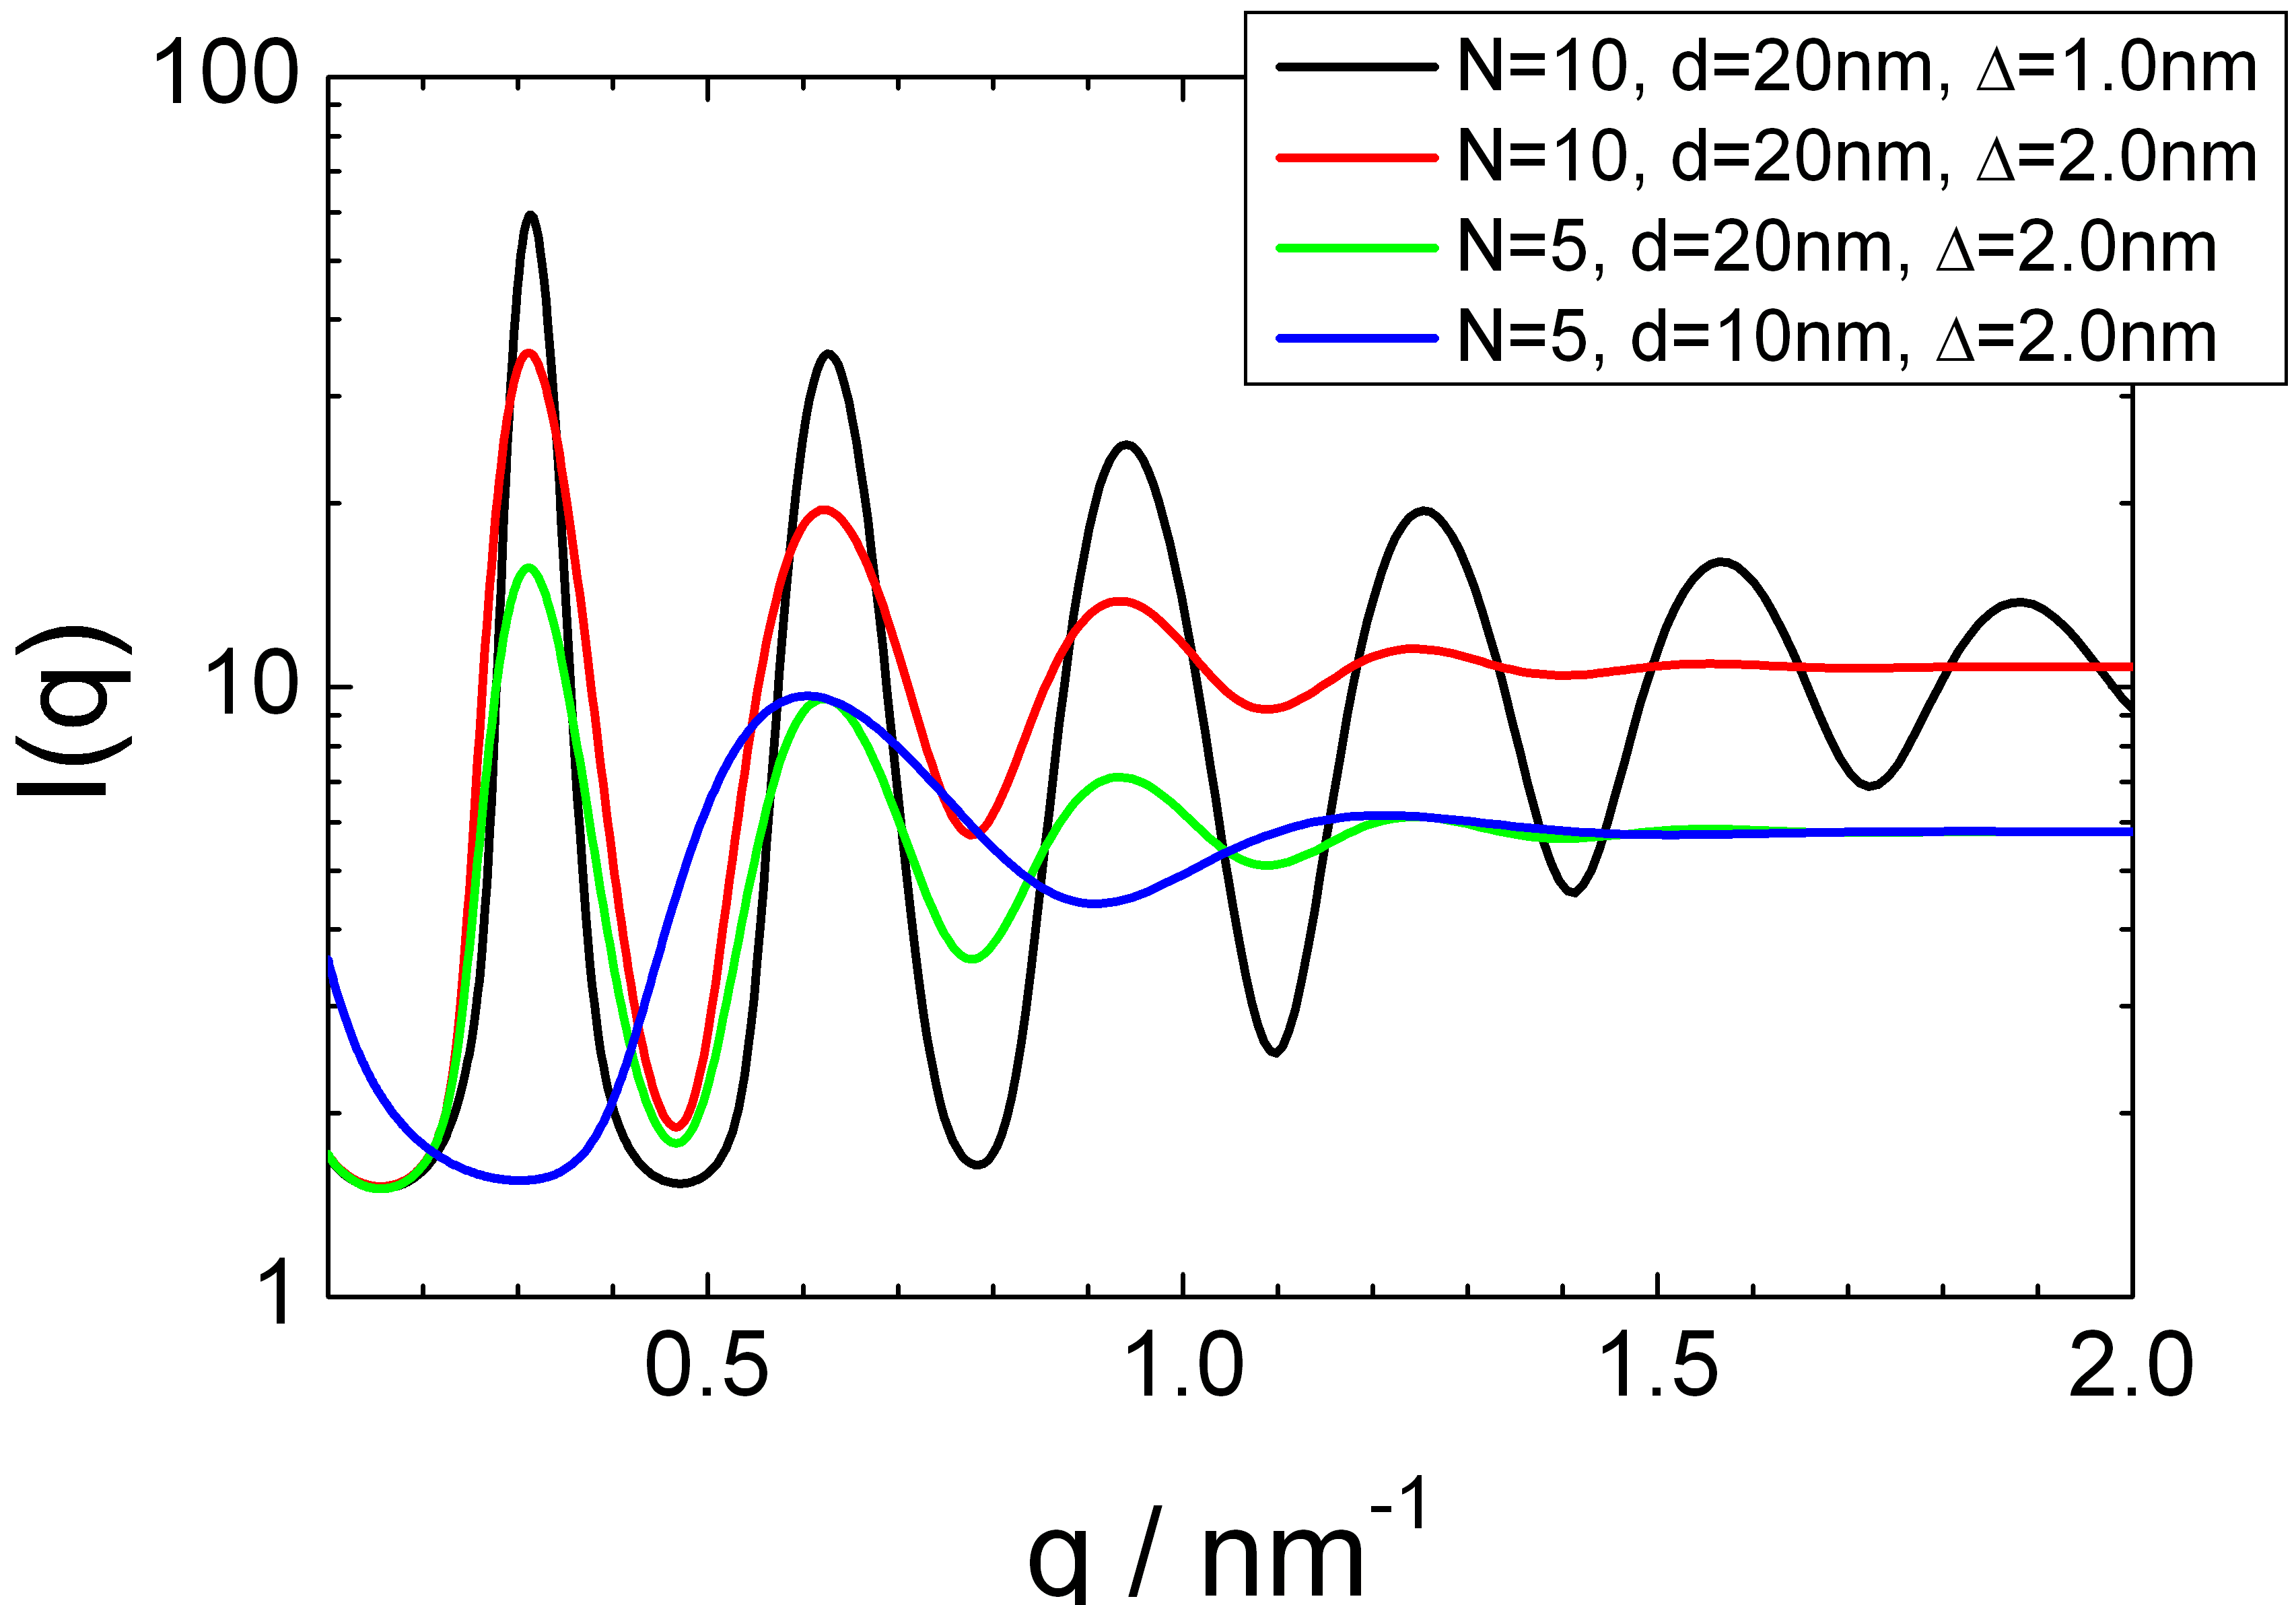
\includegraphics[width=0.65\textwidth,height=0.5\textwidth]{../images/structure_factor/Lamellar/PCLamellar.png}
\end{center}
\caption{Structure factor of multi-lamellar structures with para-crystalline disorder. }
\label{fig:PCLamellar}
\end{figure}

\vspace{5mm}

\noindent
\underline{Input Parameters for model \texttt{Paracrystalline}:}
\begin{description}
\item[\texttt{N}] mean number of stacks $N$
\item[\texttt{d}] stacking separation $d$
\item[\texttt{Delta}]  stacking disorder parameter $\Delta$
\item[\texttt{Nu}]   number of uncorrelated scattering bilayers $N_\text{diff}$
\end{description}

\noindent\underline{Note:}
\begin{itemize}
\item This structure factor is intended to be used with the \texttt{monodisperse approximation}.
\end{itemize}

%%%%%%%%%%%%%%%%%%%%%%%%%%%%%%%%%%%%%%%%%%%%%%%%%%%%%%%%%%%%%%%%%%%%%%%

\clearpage
\subsection{Multi-Lamellar Structures, Modified Caill\'e Theory} ~\\

\begin{figure}[htb]
\begin{center}
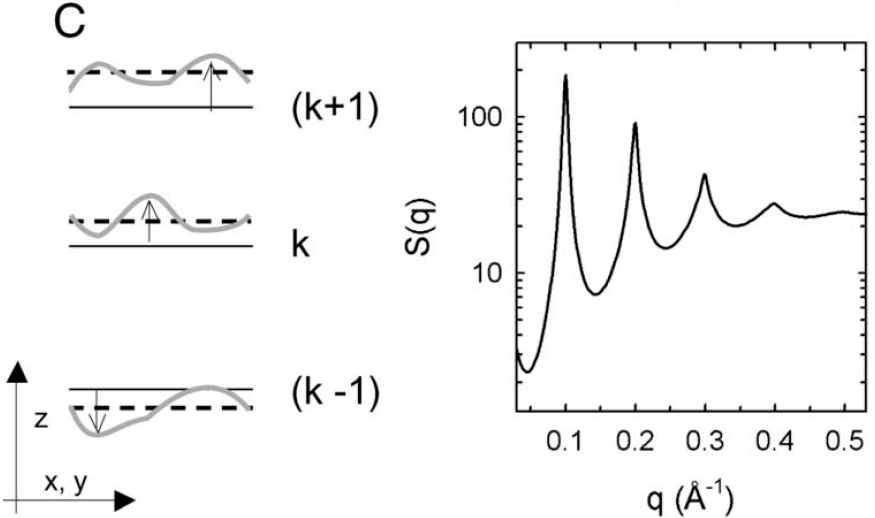
\includegraphics[width=0.7\textwidth,height=0.4\textwidth]{ModifiedCailleTheorySQ.png}
\end{center}
\caption{Bending fluctuation disorder is a particular feature of
the $L_\alpha$ (smectic A) phase and is caused by bilayer
undulations. The particular shape of the Bragg peaks is given by
the modified Caill\'e theory (MCT).}
\label{ModifiedCailleTheorySQ}
\end{figure}

There is another type of disorder when bilayer bending fluctuations
are considered (Fig. \ref{ModifiedCailleTheorySQ}). Such
fluctuations are particularly pronounced in the fluid $L_\alpha$
phase (equivalent to smectic A). Caill\'e Bending fluctuation
disorder is a particular feature of the $L_\alpha$ (smectic A) phase
and is caused by bilayer undulations. The particular shape of the
Bragg peaks is given by the modified Caill\'e theory (MCT).
\cite{Caille1972} realized the impact on the structure factor, which
in a modified version \cite{Zhang1994} of the Caill\'e theory (MCT)
is
\begin{align}
S_\text{MC}(Q,N,d,\eta_1,\gamma, N_\text{diff}) = N_\text{diff}+
\sum_{N_k=N-2\sigma}^{N+2\sigma} x_k S_\text{k,MC}
\end{align}
with
\begin{align}
S_\text{k,MC} = N_k + 2 \sum_{m=1}^{N_k-1} (N_k-m) \cos(mQd) \,\,
e^{ -\left(\frac{d}{2\pi}\right)^2 Q^2 \eta_1 \gamma } \,\, (\pi
m)^{-(d/2\pi)^2Q^2\eta_1}
\end{align}
Here, $\gamma$ is Euler's constant and
$$ \eta = \pi k_B T / 2d^2(BK_c)^{1/2}$$
is the Caill\'e parameter, which is a measure for the bilayer
fluctuations and is inversely proportional to the square root of the
bilayer bending rigidity $K_c$ times the bulk modulus of compression
$B$ (De Gennes \& Prost, 1993). Therefore, a lineshape analysis of
the quasi-Bragg peaks opens an important experimental window on
interbilayer interactions. Further, $K_c$ and $B$ can be decoupled
as demonstrated recently by hydration studies
\cite{Petrache1998,Pabst2003}, or more elegantly by measuring
multibilayers aligned on a solid substrate \cite{Lyatskaya2000}.
$N_\text{diff}$ accounts for an additional diffuse background, due
to a number of uncorrelated scattering bilayers in
$S_\text{MC}(Q,N,d,\eta_1,\gamma, N_\text{diff}) $, which is not
included in the MCT. Its origin is attributed to bilayers with
strong lattice defects or unilamellar vesicles, which display
neither short-range nor (quasi-) long-range order.

Fig. \ref{ModifiedCailleTheorySQ} shows a typical example of
$S_\text{k,MCT}(Q)$, which is similar to $S_\text{PT}(Q)$ with
respect to the progressive decrease in peak height and increase in
peak width, but which differs significantly in line shape as
$$
S_\text{k,MCT} \propto (Q-Q_h)^{-1+\eta h^2}
$$
for randomly oriented scattering domains \cite{Roux1988,Zhang1994}.


The structure factors $S_\text{k,MCT}(Q)$ with low, but fixed
stacking numbers $N$ show oscillations at low $Q$ (as can be seen in
Fig. \ref{ModifiedCailleTheorySQ}), but no such oscillations are
found in experimental data. This can be understood as the
consequence of polydispersity in the size of the different stacks.
In order to eliminate these artifacts from strictly monodisperse
systems, we use a `polydisperse' structure factor, i.e. we use an
average of a series of structure factors with varying numbers of
bilayers \cite{Fruhwirth2004}. The analytical form of the
distribution is not known a priori. We use a Gaussian distribution
approximated by a discrete series The standard deviation $\sigma$
for the Gaussian-weighted distribution is chosen as
\begin{align}
\sigma =
\begin{cases}
\sqrt{N} & \text{for} N\geq 5 \text{,} \\
0.5(N-1) & \text{for} N< 5
\end{cases}
\end{align}
Therefore, $N$ must be greater or equal to 2, which is a
reasonable restriction for multilamellar stacks of bilayers. In
the range of $N \pm 2\sigma$, structure factors weighted by
\begin{align}
x_k & = \frac{1}{\sigma\sqrt{2\pi}} \exp\left[
-\frac{(N_k-N)^2}{2\sigma^2}\right]
\end{align}
are calculated, where $N$ is the mean number of stacks and $N_k$
is one of the  bilayers in the range $N\pm 2\sigma$. This
polydispersity model does not introduce new free parameters and is
symmetrical around the mean $N$.

\begin{figure}[htb]
\begin{center}
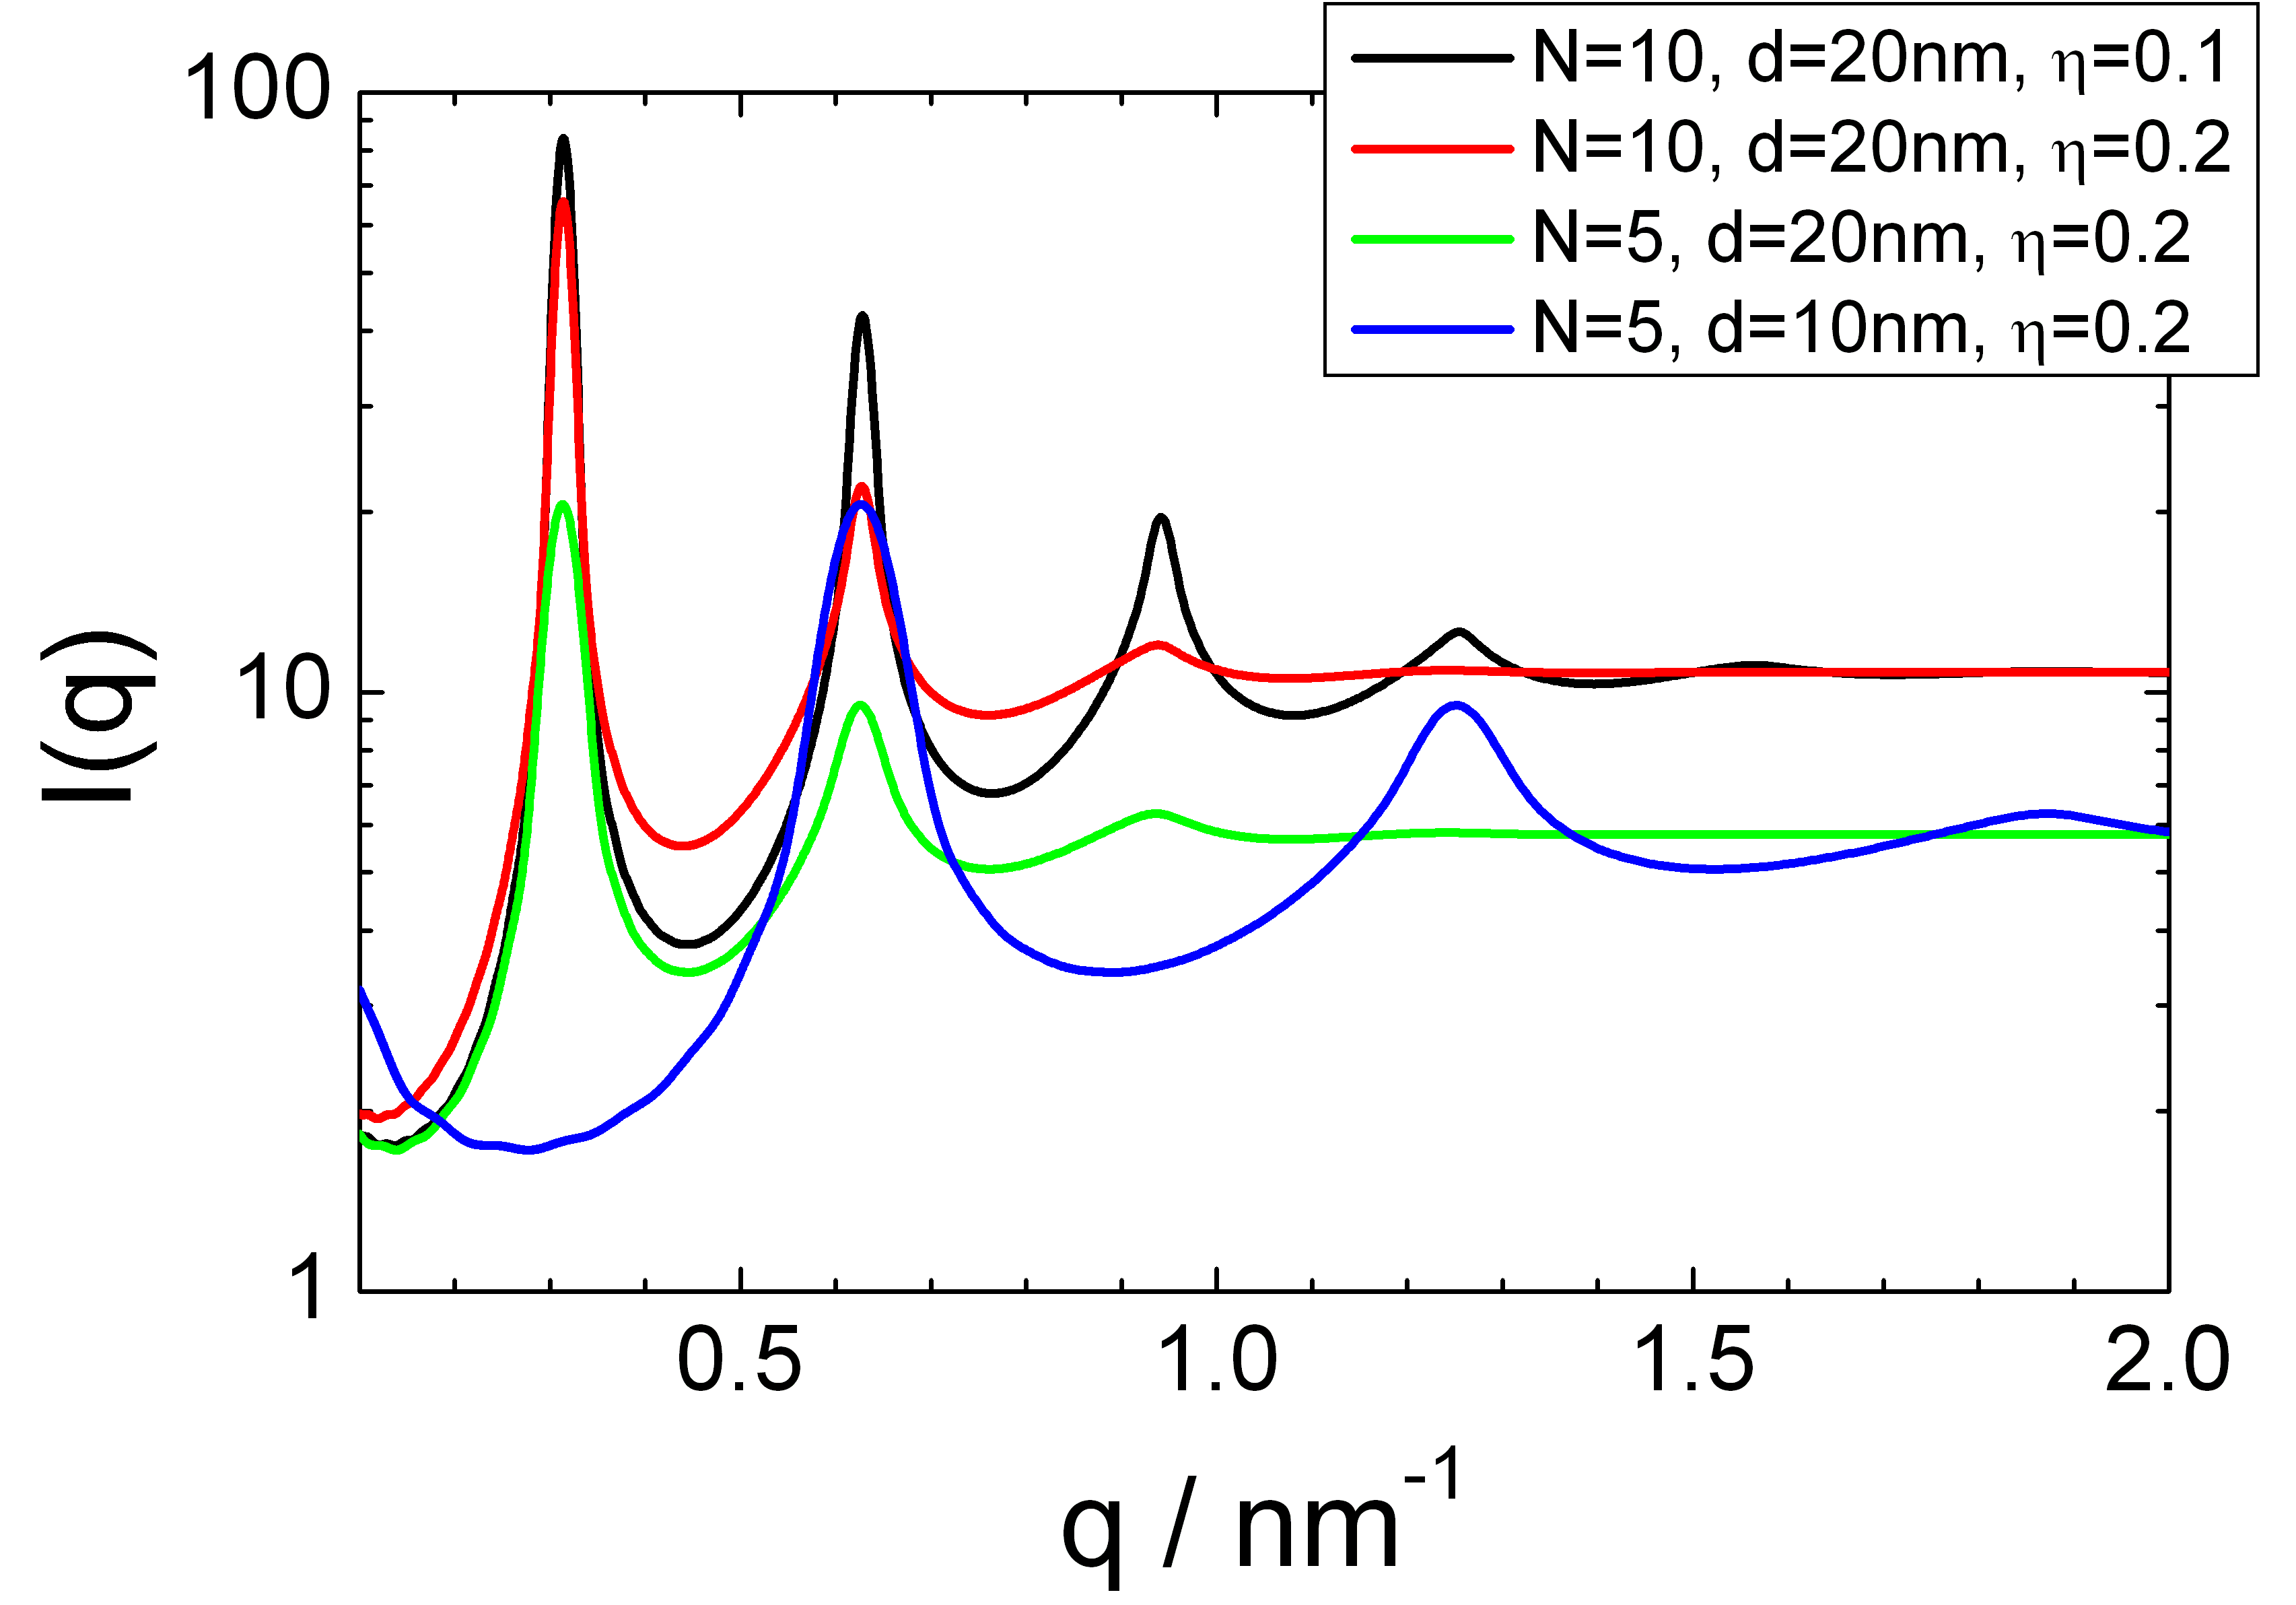
\includegraphics[width=0.65\textwidth,height=0.5\textwidth]{../images/structure_factor/Lamellar/MCLamellar.png}
\end{center}
\caption{Structure factor of multi-lamellar structures according to the modified Caill\'e theory.}
\label{fig:MCLamellar}
\end{figure}

\vspace{5mm}

\noindent
\underline{Input Parameters for model \texttt{ModifiedCaile}:}
\begin{description}
\item[\texttt{N}] mean number of stacks $N$
\item[\texttt{d}] stacking separation $d$
\item[\texttt{eta}]  the Caill\'e parameter $\eta$ is a measure for the bilayer
fluctuations and inversely proportional to the square root of
the bilayer bending rigidity
\item[\texttt{Nu}]   number of uncorrelated scattering bilayers $N_\text{diff}$
\end{description}

\noindent\underline{Note:}
\begin{itemize}
\item This structure factor is intended to be used with the \texttt{monodisperse approximation}.
\end{itemize}

%%%%%%%%%%%%%%%%%%%%%%%%%%%%%%%%%%%%%%%%%%%%%%%%%%%%%%%%%%%%%%%%%%%%%%%%%%%%%%%%%%%%%

\clearpage
\section{Mass Fractal}~\\
\label{sect:SQ4clusteraggregates}
For a fractal object, the structure factor $S(q)$ can be calculated
\cite{Sorensen1999,Sorensen1992} via
the pair correlation function $g(r)$, which describes the total number of
particles within a sphere of radius $r$ centered in a central
particle and is given (for $\dim = 3$) by
\begin{align}
N(r) = \Phi \int_0^r g(r) \, 4\pi r^2 \, dr
\end{align}
or
\begin{align}
\textrm{d}N(r) = \Phi  g(r) \, 4\pi r^2 \, dr \label{eq:fractdN}
\end{align}
On the other hand, a fractal object is characterized by a spatial
distribution of the individual scatterers given by
\begin{align}
N(r) = \left( \frac{r}{r_0} \right)^D \label{eq:fractN}
\end{align}
where $r_0$ is the gauge of the measurement, which has
the magnitude of the characteristic dimension of each
individual scatterer.
Differentiation of \ref{eq:fractN} and identification with \ref{eq:fractdN}
gives
\begin{align}
\Phi g(r) = \frac{D}{4\pi r_0^D} r^{D-3}
\end{align}
Because $D$ is smaller than 3, $g(r)$ goes to zero at
large $r$. This is clearly unphysical.
At some large scale, the sample will show a
macroscopic density. A good knowledge of the sample
allows in general a reasonable assumption for the
large-scale behavior of $g(r)$. Therefore a cut-off function
$h(r,\xi)$ has to be introduced, where $\xi$ is a cut-off distance, to
describe the behavior of the pair correlation function
at large distances. To derive the analytical form of
$S(q)$ within this assumption, one can use the general
theory of liquids, where the uniform density is subtracted
to avoid a divergence in the evaluation of $S(q)$.
We then write
\begin{align}
4\pi\Phi[g(r)-1] = \frac{D}{r_0^D} \, r^{D-3} h(r,\xi)
\label{eq:fract_g(r)-1}
\end{align}
The meaning of $\xi$ is only qualitative and has to be
made precise in any particular situation. Generally
speaking, it represents the characteristic distance
above which the mass distribution in the sample is no
longer described by the fractal law. In practice, it can
represent the size of an aggregate or a correlation
length in a disordered material.
For isotropic systems
\begin{align}
S(q) = 1+4\pi\Phi\int_0^\infty [g(r)-1] \frac{\sin(qr)}{qr} \, r^2 \, dr
\end{align}
Combined with \ref{eq:fract_g(r)-1} one gets
\begin{align}
S(q) = 1 +\frac{D}{r_0^D} \int_0^\infty r^{D-3} h(r,\xi)  \frac{\sin(qr)}{qr}\, r^2 \, dr
\label{eq:hSQ}
\end{align}
Several cut-off functions $h(r,\xi)$ have been discussed in the
literature and compared by Sorensen et al.\
\cite{Sorensen1999,Sorensen1992}.
\begin{align}
h_\text{Exp}(r,\xi)     &= \exp\left[-\tfrac{r}{\xi}\right] \label{eq:hExp}\\
h_\text{Gauss}(r,\xi)   &= \exp\left[-\left(\tfrac{r}{\xi}\right)^2\right] \label{eq:hGauss}\\
h_\text{Exp(-x$\hat{~}$a)}(r,\xi,\alpha,D) &= \exp\left[-\left(\tfrac{r}{\xi}\right)^\alpha\right] \label{eq:hExpmxa}\\
h_\text{OverlapSph}(r,\xi)   &=
\begin{cases}
%\left(\frac{4}{3}\pi\xi\right)
\left(1+\frac{r}{4\xi}\right)\left(1-\frac{r}{2\xi}\right)^2
& \text{for } r\leq 2\xi \\
0 & \text{for } r>2\xi
\end{cases}
\label{eq:hOverlapSph}
\end{align}
For the cut-off functions \ref{eq:hExp} and \ref{eq:hGauss} the integral \ref{eq:hSQ} can be solved
analytically and the corresponding structure factors are given by
\begin{align}
S_\text{Exp}(q,\xi,D,r_0) &= 1 +  \cfrac{D \Gamma(D-1)
\sin\left([D-1]\arctan(q \xi)\right)}{\left( q r_0\right)^D
\left[1+\tfrac{1}{q^2\xi^2}\right]^{(D-1)/2}} \\
S_\text{Gauss}(q,\xi,D,r_0) &= 1 +
    \Gamma\left[\tfrac{D}{2}\right]\frac{D}{2}
    \left(\frac{\xi}{r_0}\right)^D
    {}_1F_1\left[\tfrac{D}{2},\tfrac{3}{2},-\tfrac{q^2\xi^2}{8}\right]
\end{align}
where $D$ is the fractal dimension, $\xi$ is a cut-off length for
the fractal correlations, $\Gamma(x)$ is the gamma function.
${}_1F_1\left[\right]$ is the Kummer or hypergeometric function. For
the cut-off functions \ref{eq:hExpmxa} and \ref{eq:hOverlapSph} the
integral \ref{eq:hSQ} is solved numerically.

\begin{figure}[htb]
\begin{center}
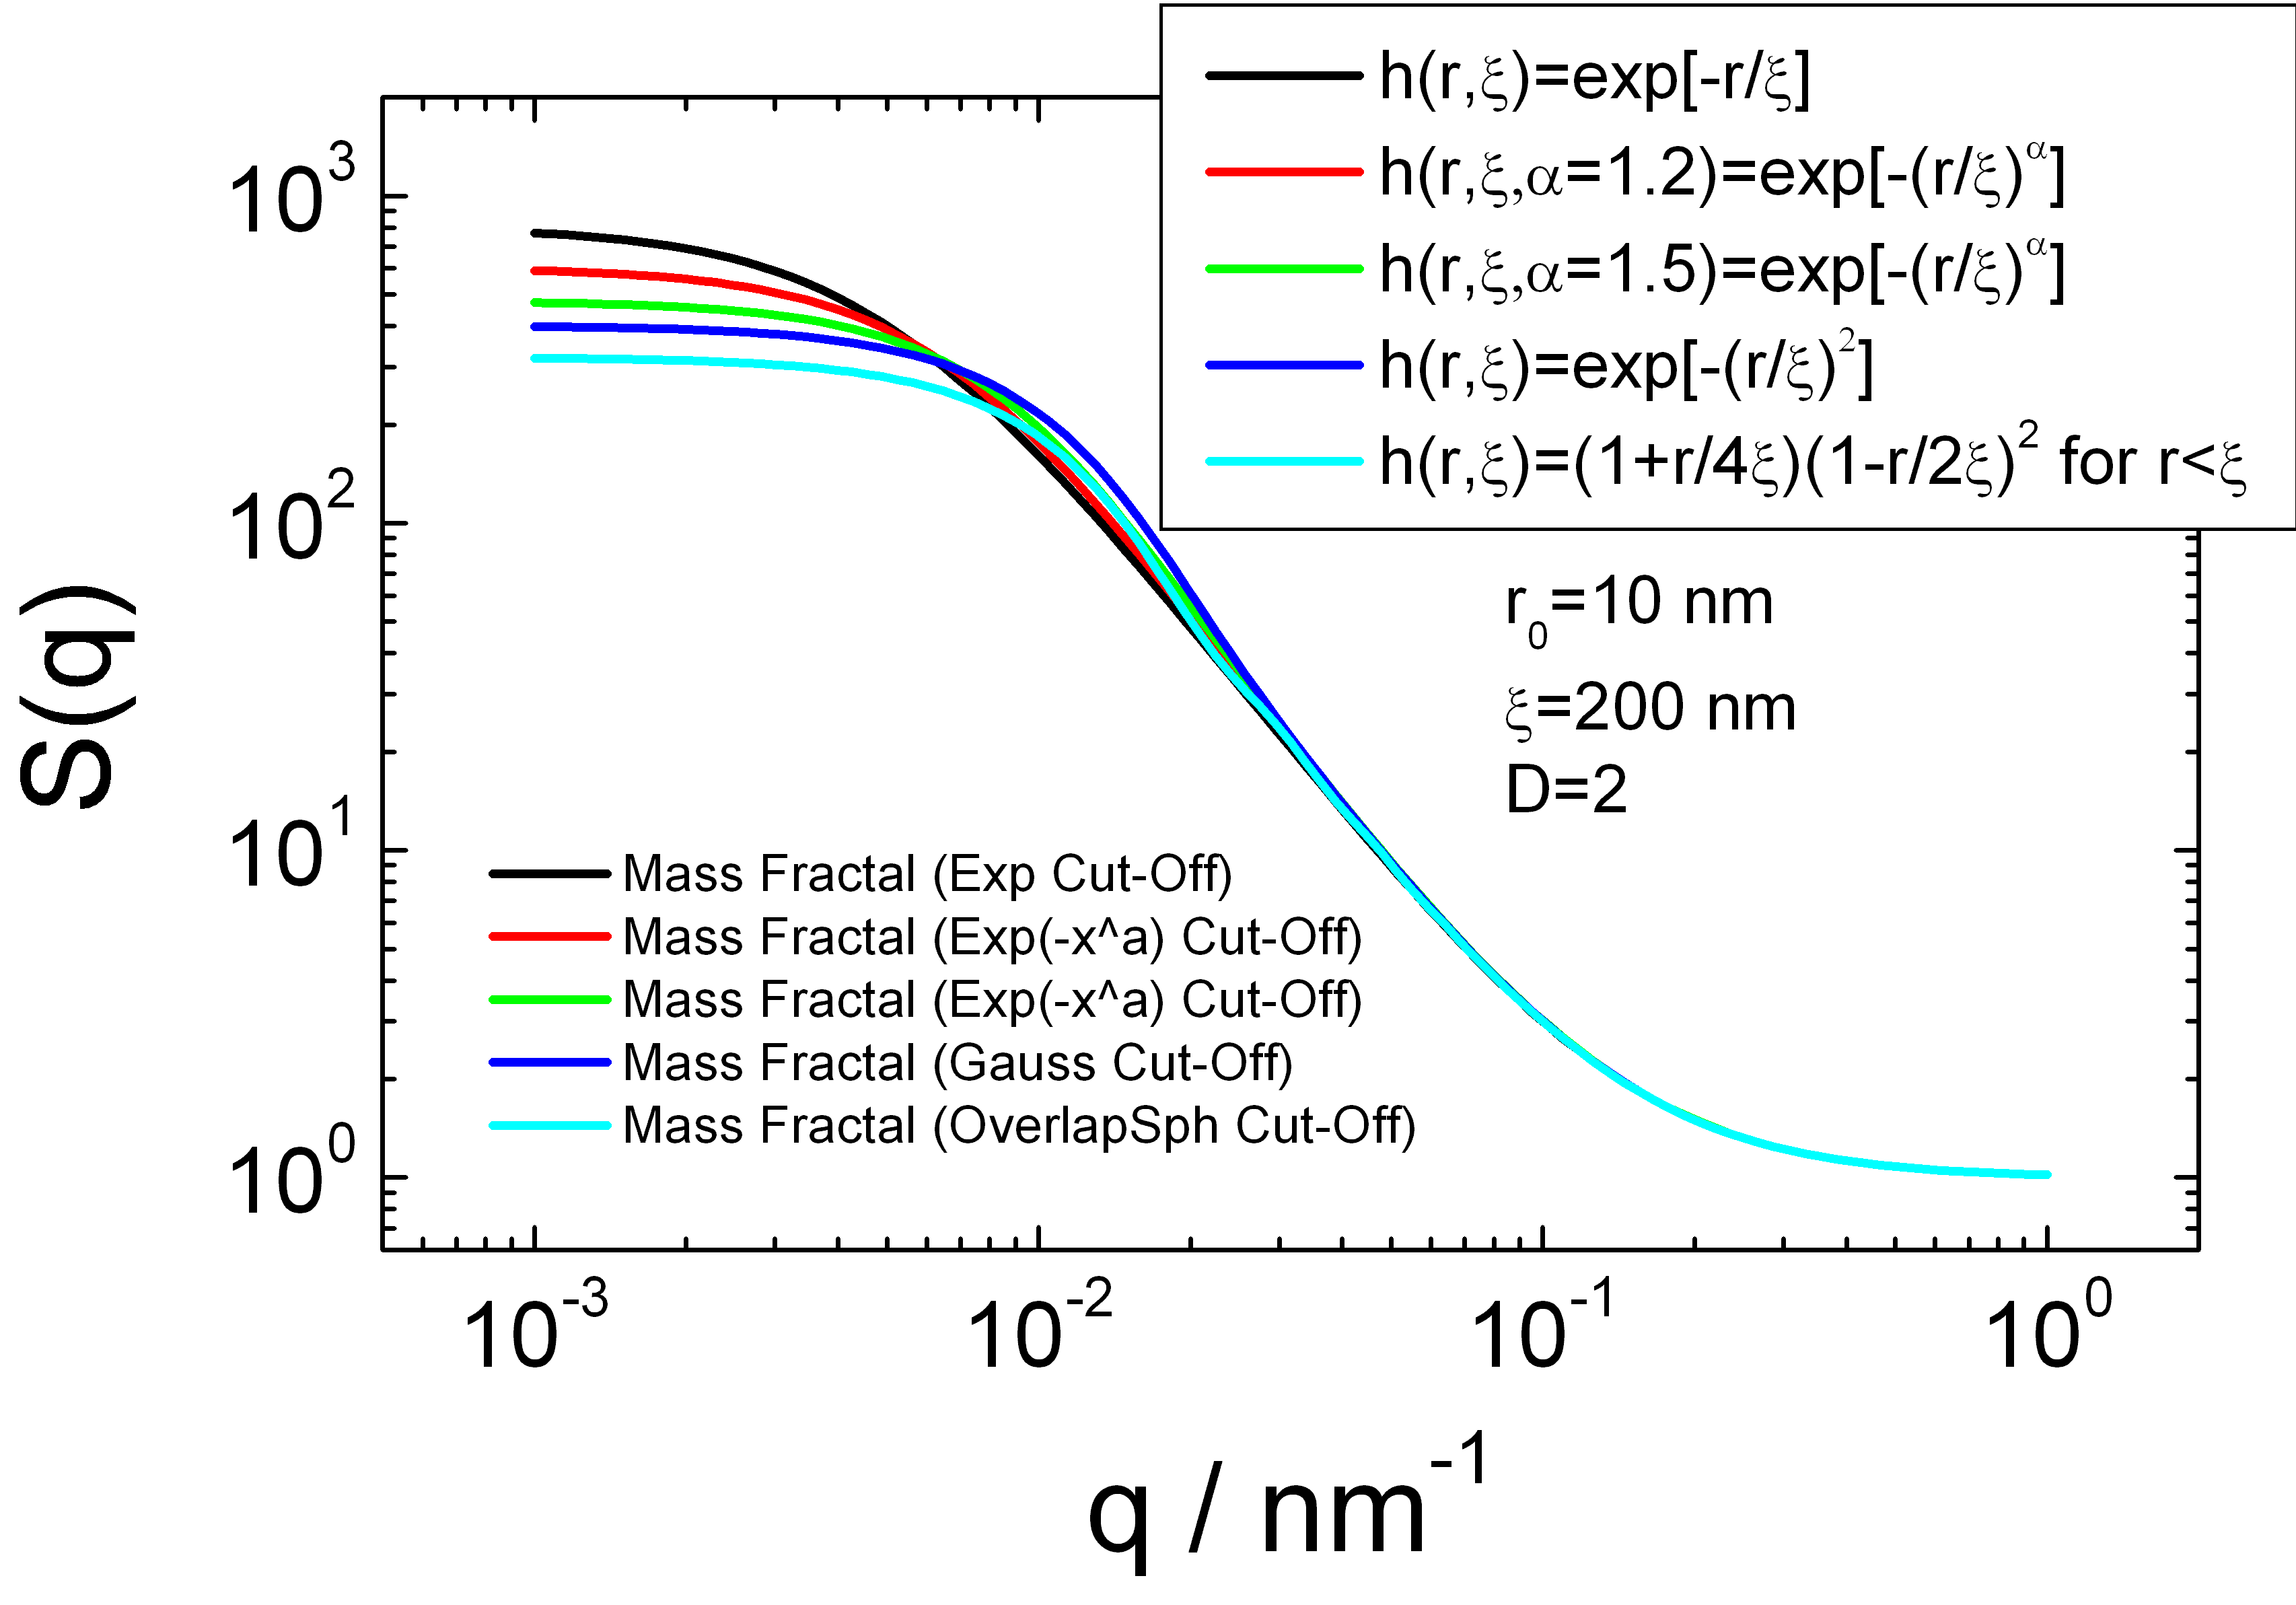
\includegraphics[width=0.768\textwidth,height=0.488\textwidth]{../images/structure_factor/MassFractals/ComparingSQMassFractals.png}
\end{center}
\caption{Comparison of the different structure factors for mass
fractals.} \label{fig:MassFractCompare}
\end{figure}


\clearpage
\subsection{Mass Fractal (Exp Cut-Off)}
~\\

\underline{Input Parameters for model \texttt{Mass Fractal (Exp Cut-Off)}:}
\begin{description}
\item[\texttt{r0}] characteristic dimension of individual scattering objects $r_0$
\item[\texttt{xi}] cut-off length for the fractal correlations $\xi$
\item[\texttt{D}] fractal dimension $D$
\end{description}

\underline{Note:}
\begin{itemize}
\item $D$ needs to be larger than 1 ($D>1$). Physical values for $D$ are between 1 and 3 ($1<D<3$).
\item The fractal dimension needs to be large than the size of the individual scattering objects ($r_0 < \xi$).
\end{itemize}

\begin{figure}[htb]
\begin{center}
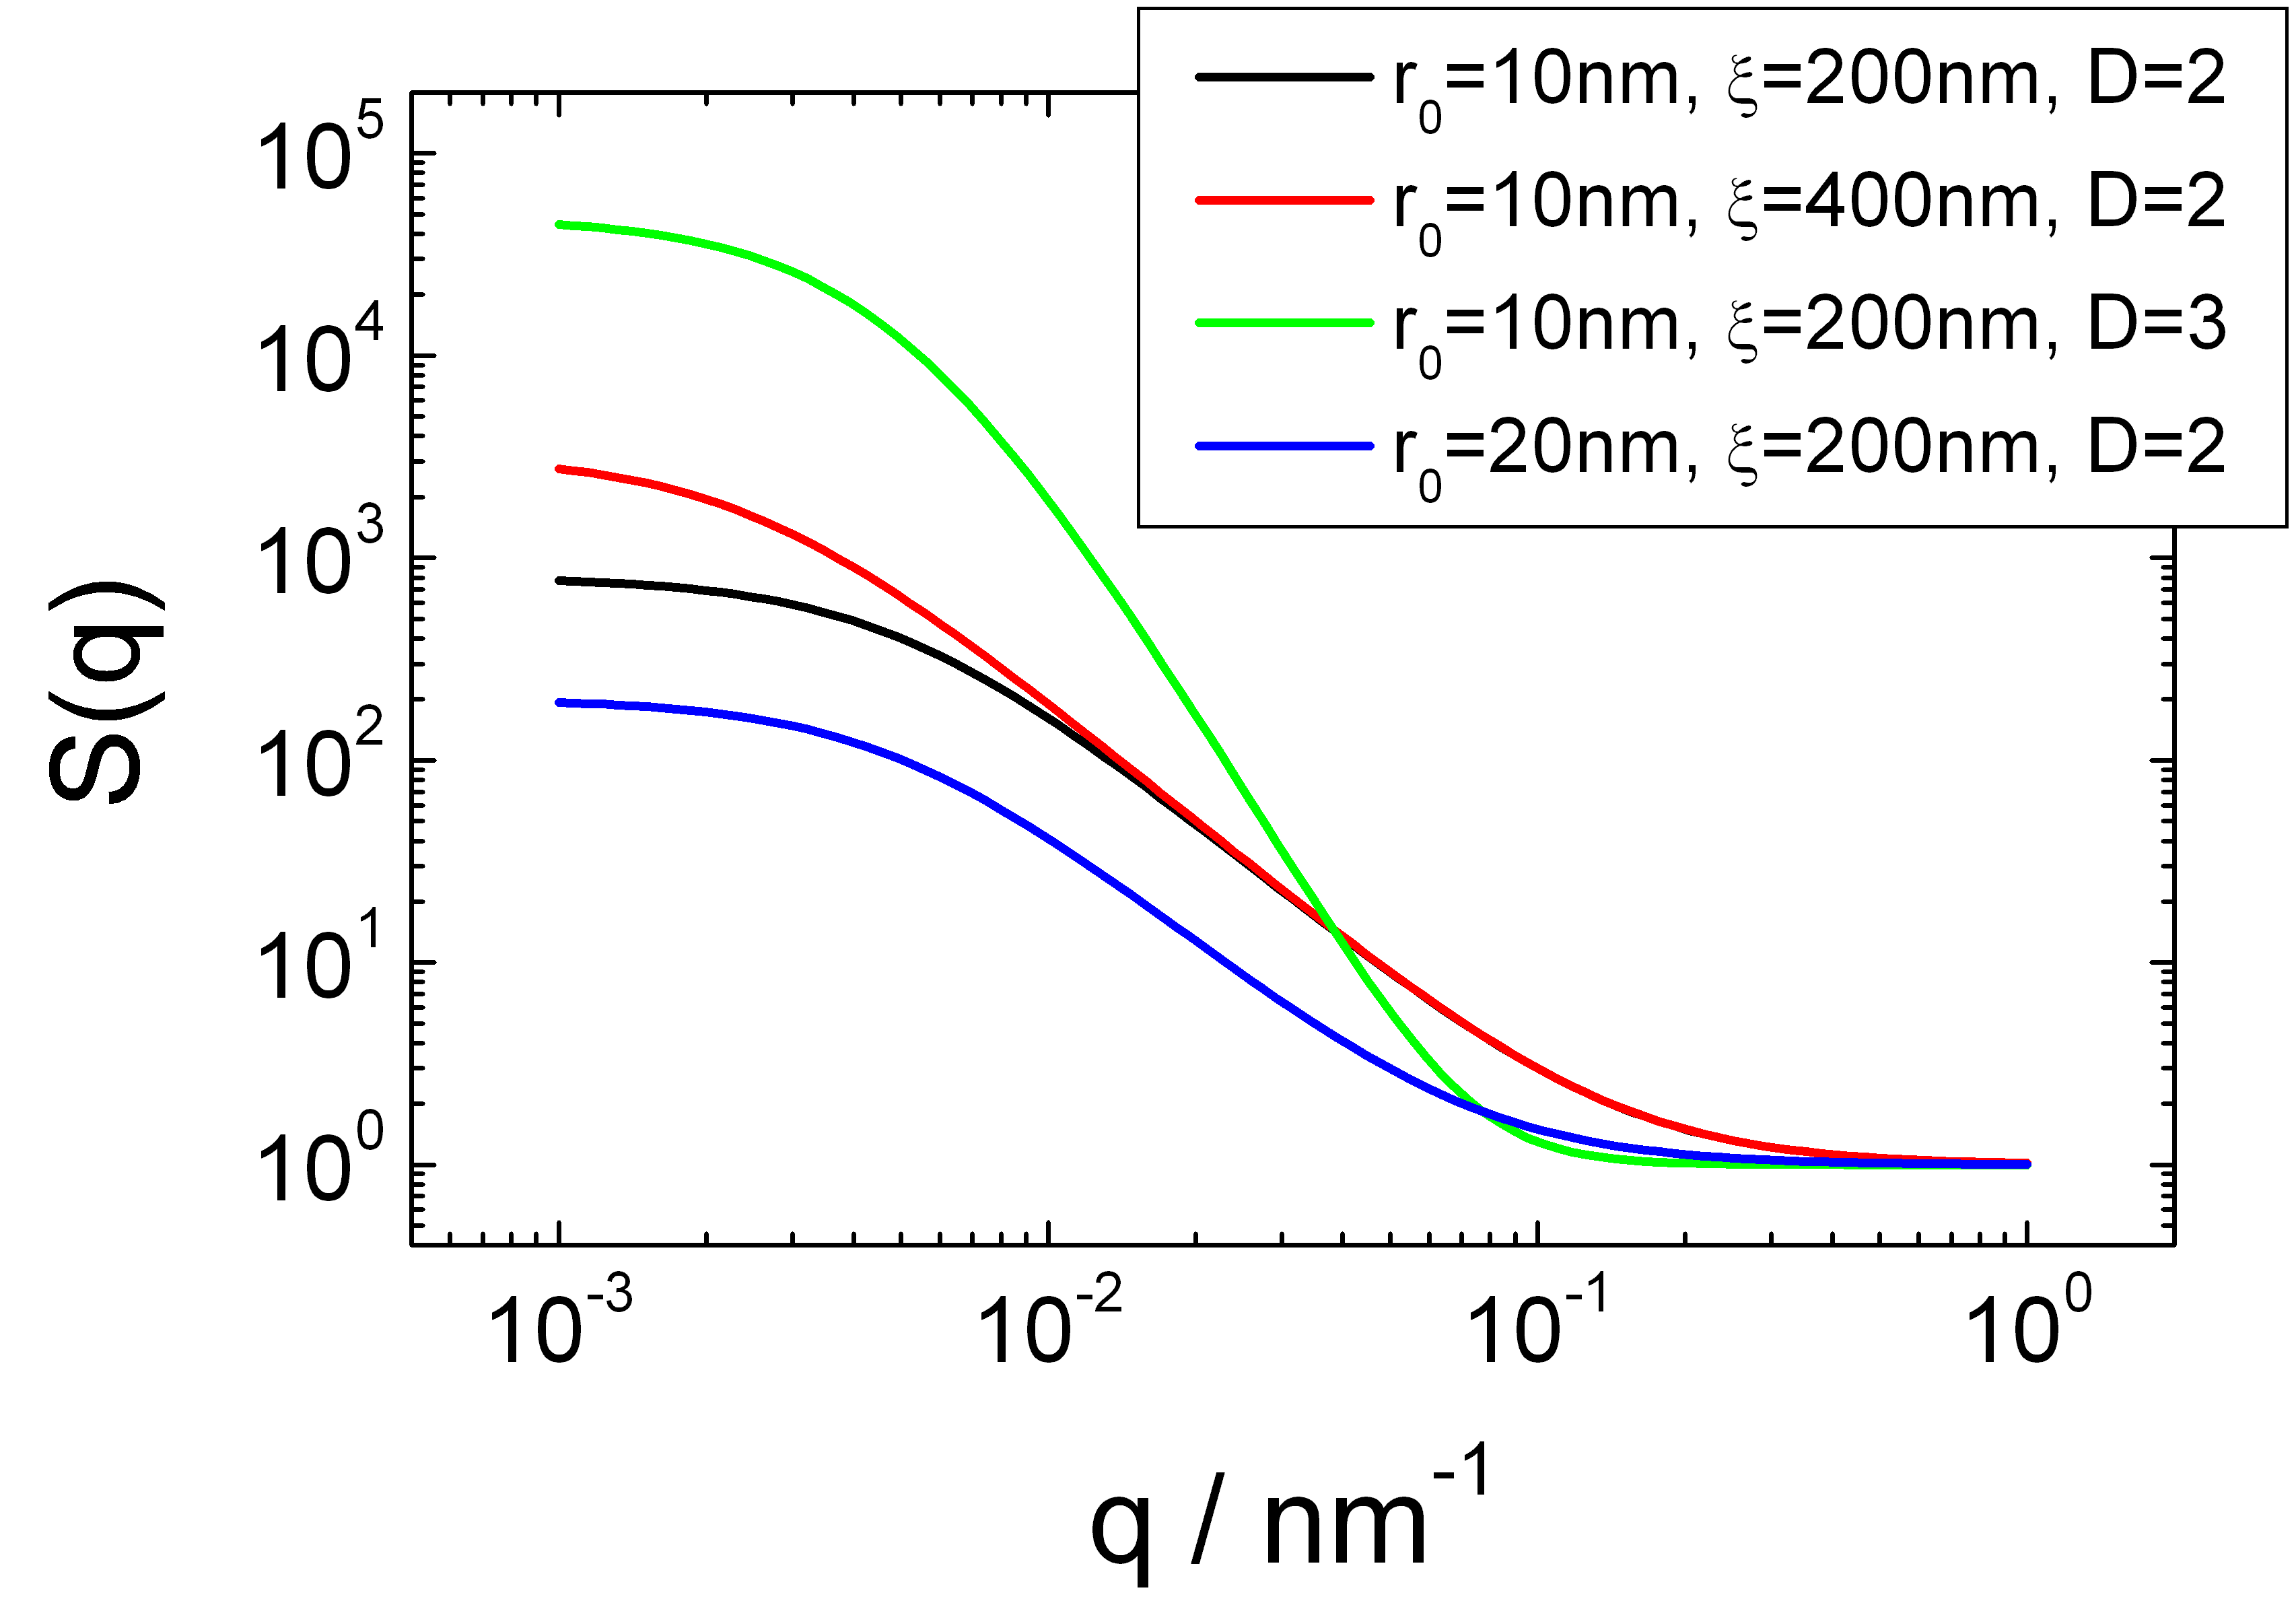
\includegraphics[width=0.768\textwidth,height=0.488\textwidth]{../images/structure_factor/MassFractals/SQExpCutOff.png}
\end{center}
\caption{Structure factor of a mass fractal with an exponential
cut-off function $h_\text{Exp}(r,\xi) = \exp\left[-\left(\tfrac{r}{\xi}\right)^\alpha\right]$.}
\label{fig:SQExpCutOff}
\end{figure}


\clearpage
\subsection{Mass Fractal (Exp(-x\^{}a) Cut-Off)}
~\\

\underline{Input Parameters for model \texttt{Mass Fractal (Exp(-x\^{}a) Cut-Off)}:}
\begin{description}
\item[\texttt{r0}] characteristic dimension of individual scattering objects $r_0$
\item[\texttt{xi}] cut-off length for the fractal correlations $\xi$
\item[\texttt{D}] fractal dimension $D$
\end{description}

\underline{Note:}
\begin{itemize}
\item $D$ needs to be larger than 1 ($D>1$). Physical values for $D$ are between 1 and 3 ($1<D<3$).
\item The fractal dimension needs to be large than the size of the individual scattering objects ($r_0 < \xi$).
\item the exponents $\alpha$ should be larger than 1, as otherwise the integral \ref{eq:hSQ} for $S(q)$ does not converges.
\end{itemize}

\begin{figure}[htb]
\begin{center}
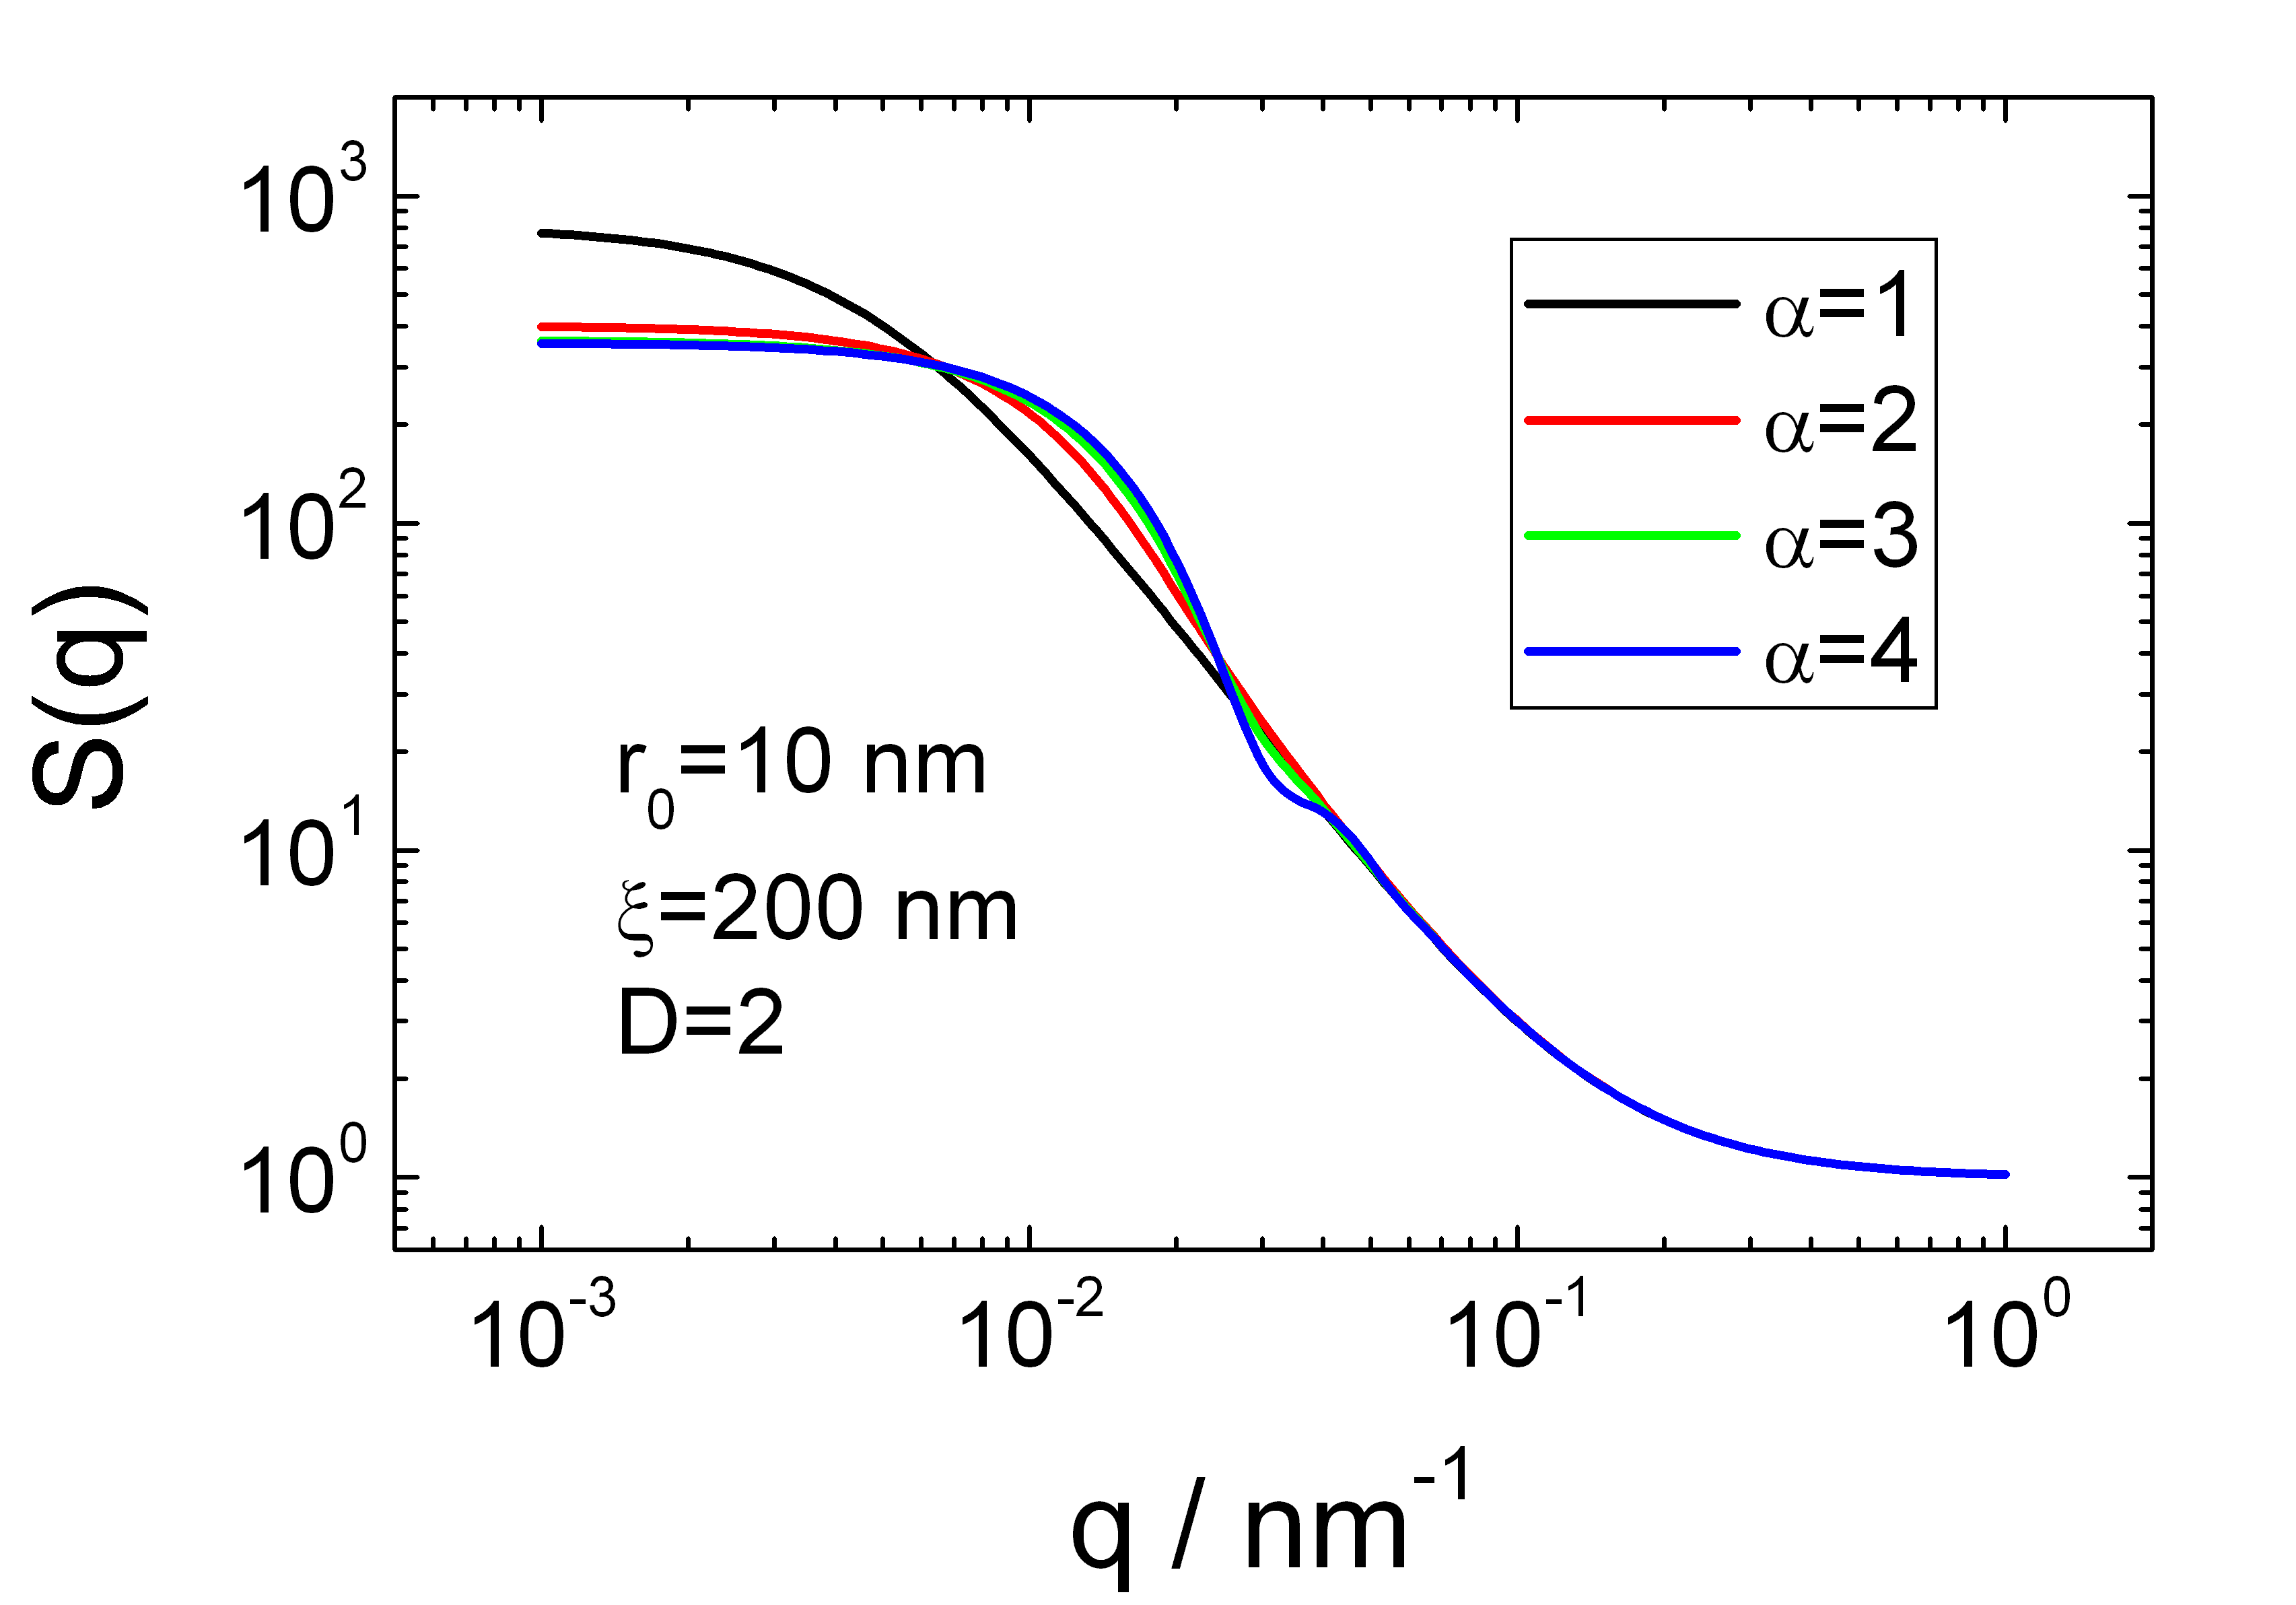
\includegraphics[width=0.768\textwidth,height=0.488\textwidth]{../images/structure_factor/MassFractals/SQExp(pow(x,a))CutOff.png}
\end{center}
\caption{Structure factor of a mass fractal with a cut-off function
$h_\text{Exp(-x$\hat{~}$a)}(r,\xi,\alpha) = \exp\left[-\left(\tfrac{r}{\xi}\right)^\alpha\right]$.}
\label{fig:SQExpxaCutOff}
\end{figure}


\clearpage
\subsection{Mass Fractal (Gaussian Cut-Off)}
~\\

\underline{Input Parameters for model \texttt{Mass Fractal (Gaussian Cut-Off)}:}
\begin{description}
\item[\texttt{r0}] characteristic dimension of individual scattering objects $r_0$
\item[\texttt{xi}] cut-off length for the fractal correlations $\xi$
\item[\texttt{D}] fractal dimension $D$
\end{description}

\underline{Note:}
\begin{itemize}
\item $D$ needs to be larger than 1 ($D>1$). Physical values for $D$ are between 1 and 3 ($1<D<3$).
\item The fractal dimension needs to be large than the size of the individual scattering objects ($r_0 < \xi$).
\end{itemize}

\begin{figure}[htb]
\begin{center}
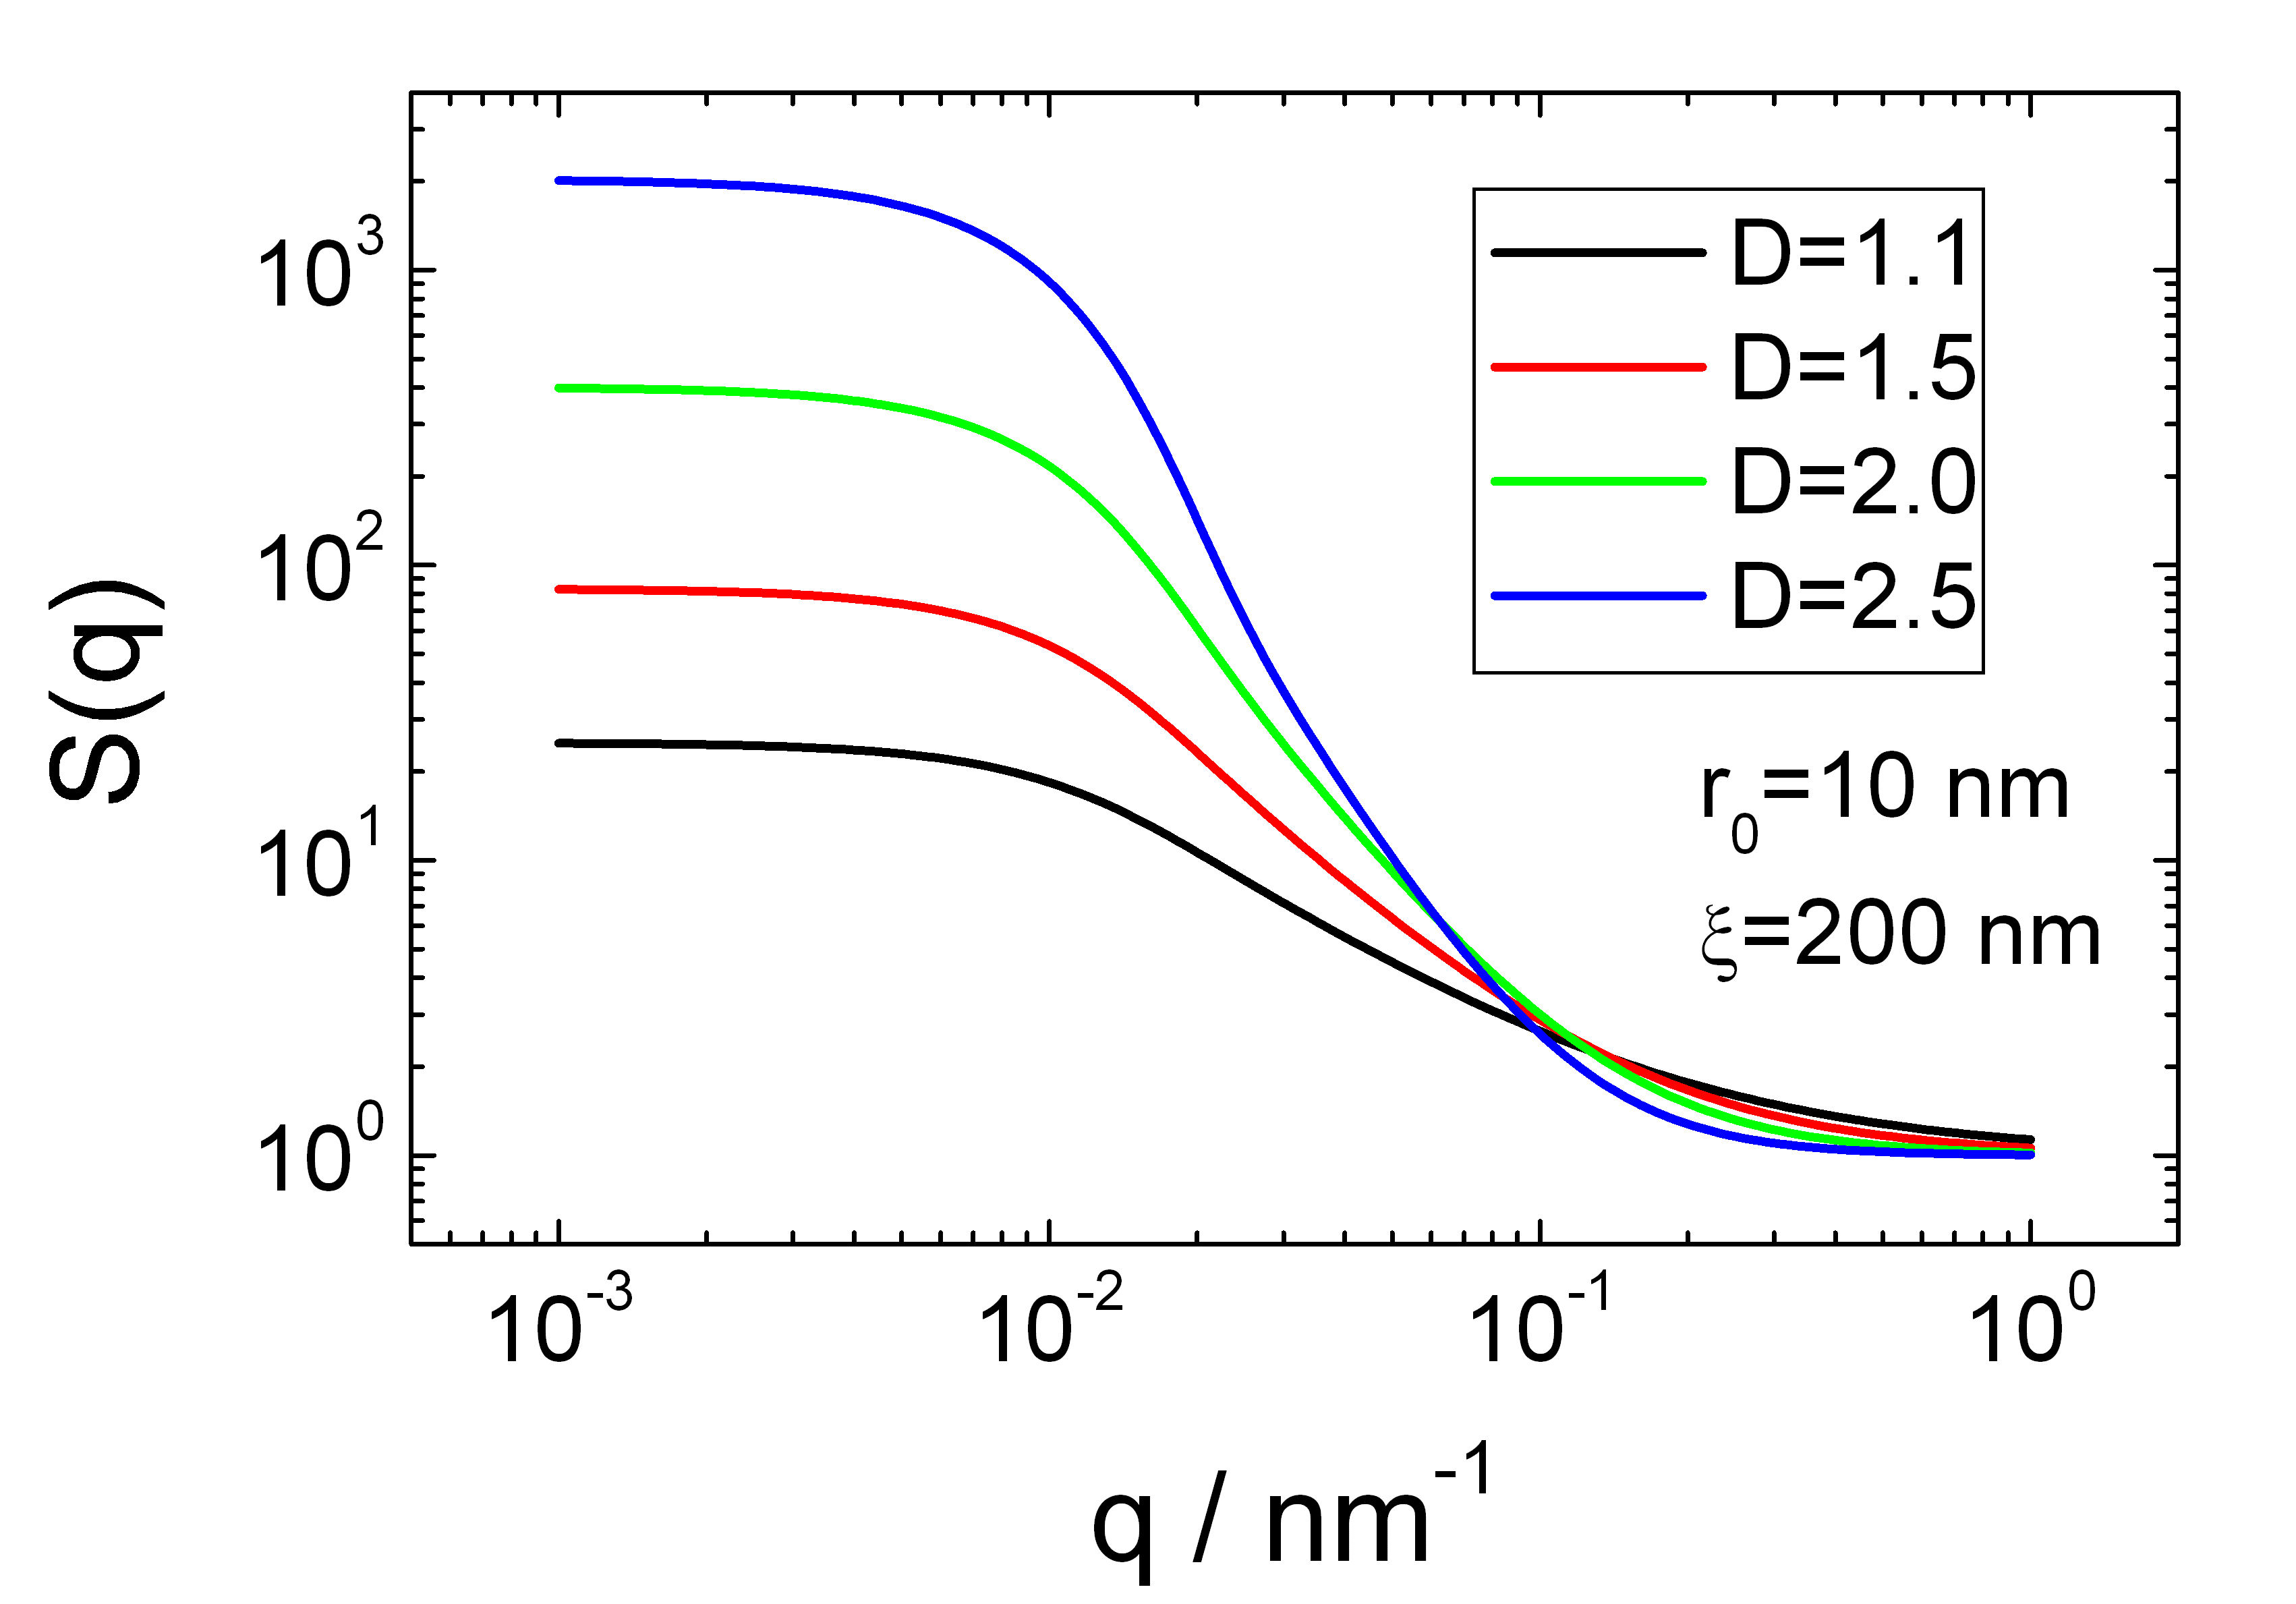
\includegraphics[width=0.768\textwidth,height=0.488\textwidth]{../images/structure_factor/MassFractals/SQGaussCutOff.png}
\end{center}
\caption{Structure factor of a mass fractal with an Gaussian
cut-off function $h_\text{Gauss}(r,\xi) = \exp\left[-\left(\tfrac{r}{\xi}\right)^2\right]$.}
\label{fig:SQGaussCutOff}
\end{figure}


\clearpage
\subsection{Mass Fractal (OverlapSph Cut-Off)}
~\\

\underline{Input Parameters for model \texttt{Mass Fractal (OverlapSph Cut-Off)}:}
\begin{description}
\item[\texttt{r0}] characteristic dimension of individual scattering objects $r_0$
\item[\texttt{xi}] cut-off length for the fractal correlations $\xi$
\item[\texttt{D}] fractal dimension $D$
\end{description}

\underline{Note:}
\begin{itemize}
\item $D$ needs to be between 1 and 3 ($1<D<3$).
\item The fractal dimension needs to be large than the size of the individual scattering objects ($r_0 < \xi$).
\end{itemize}

\begin{figure}[htb]
\begin{center}
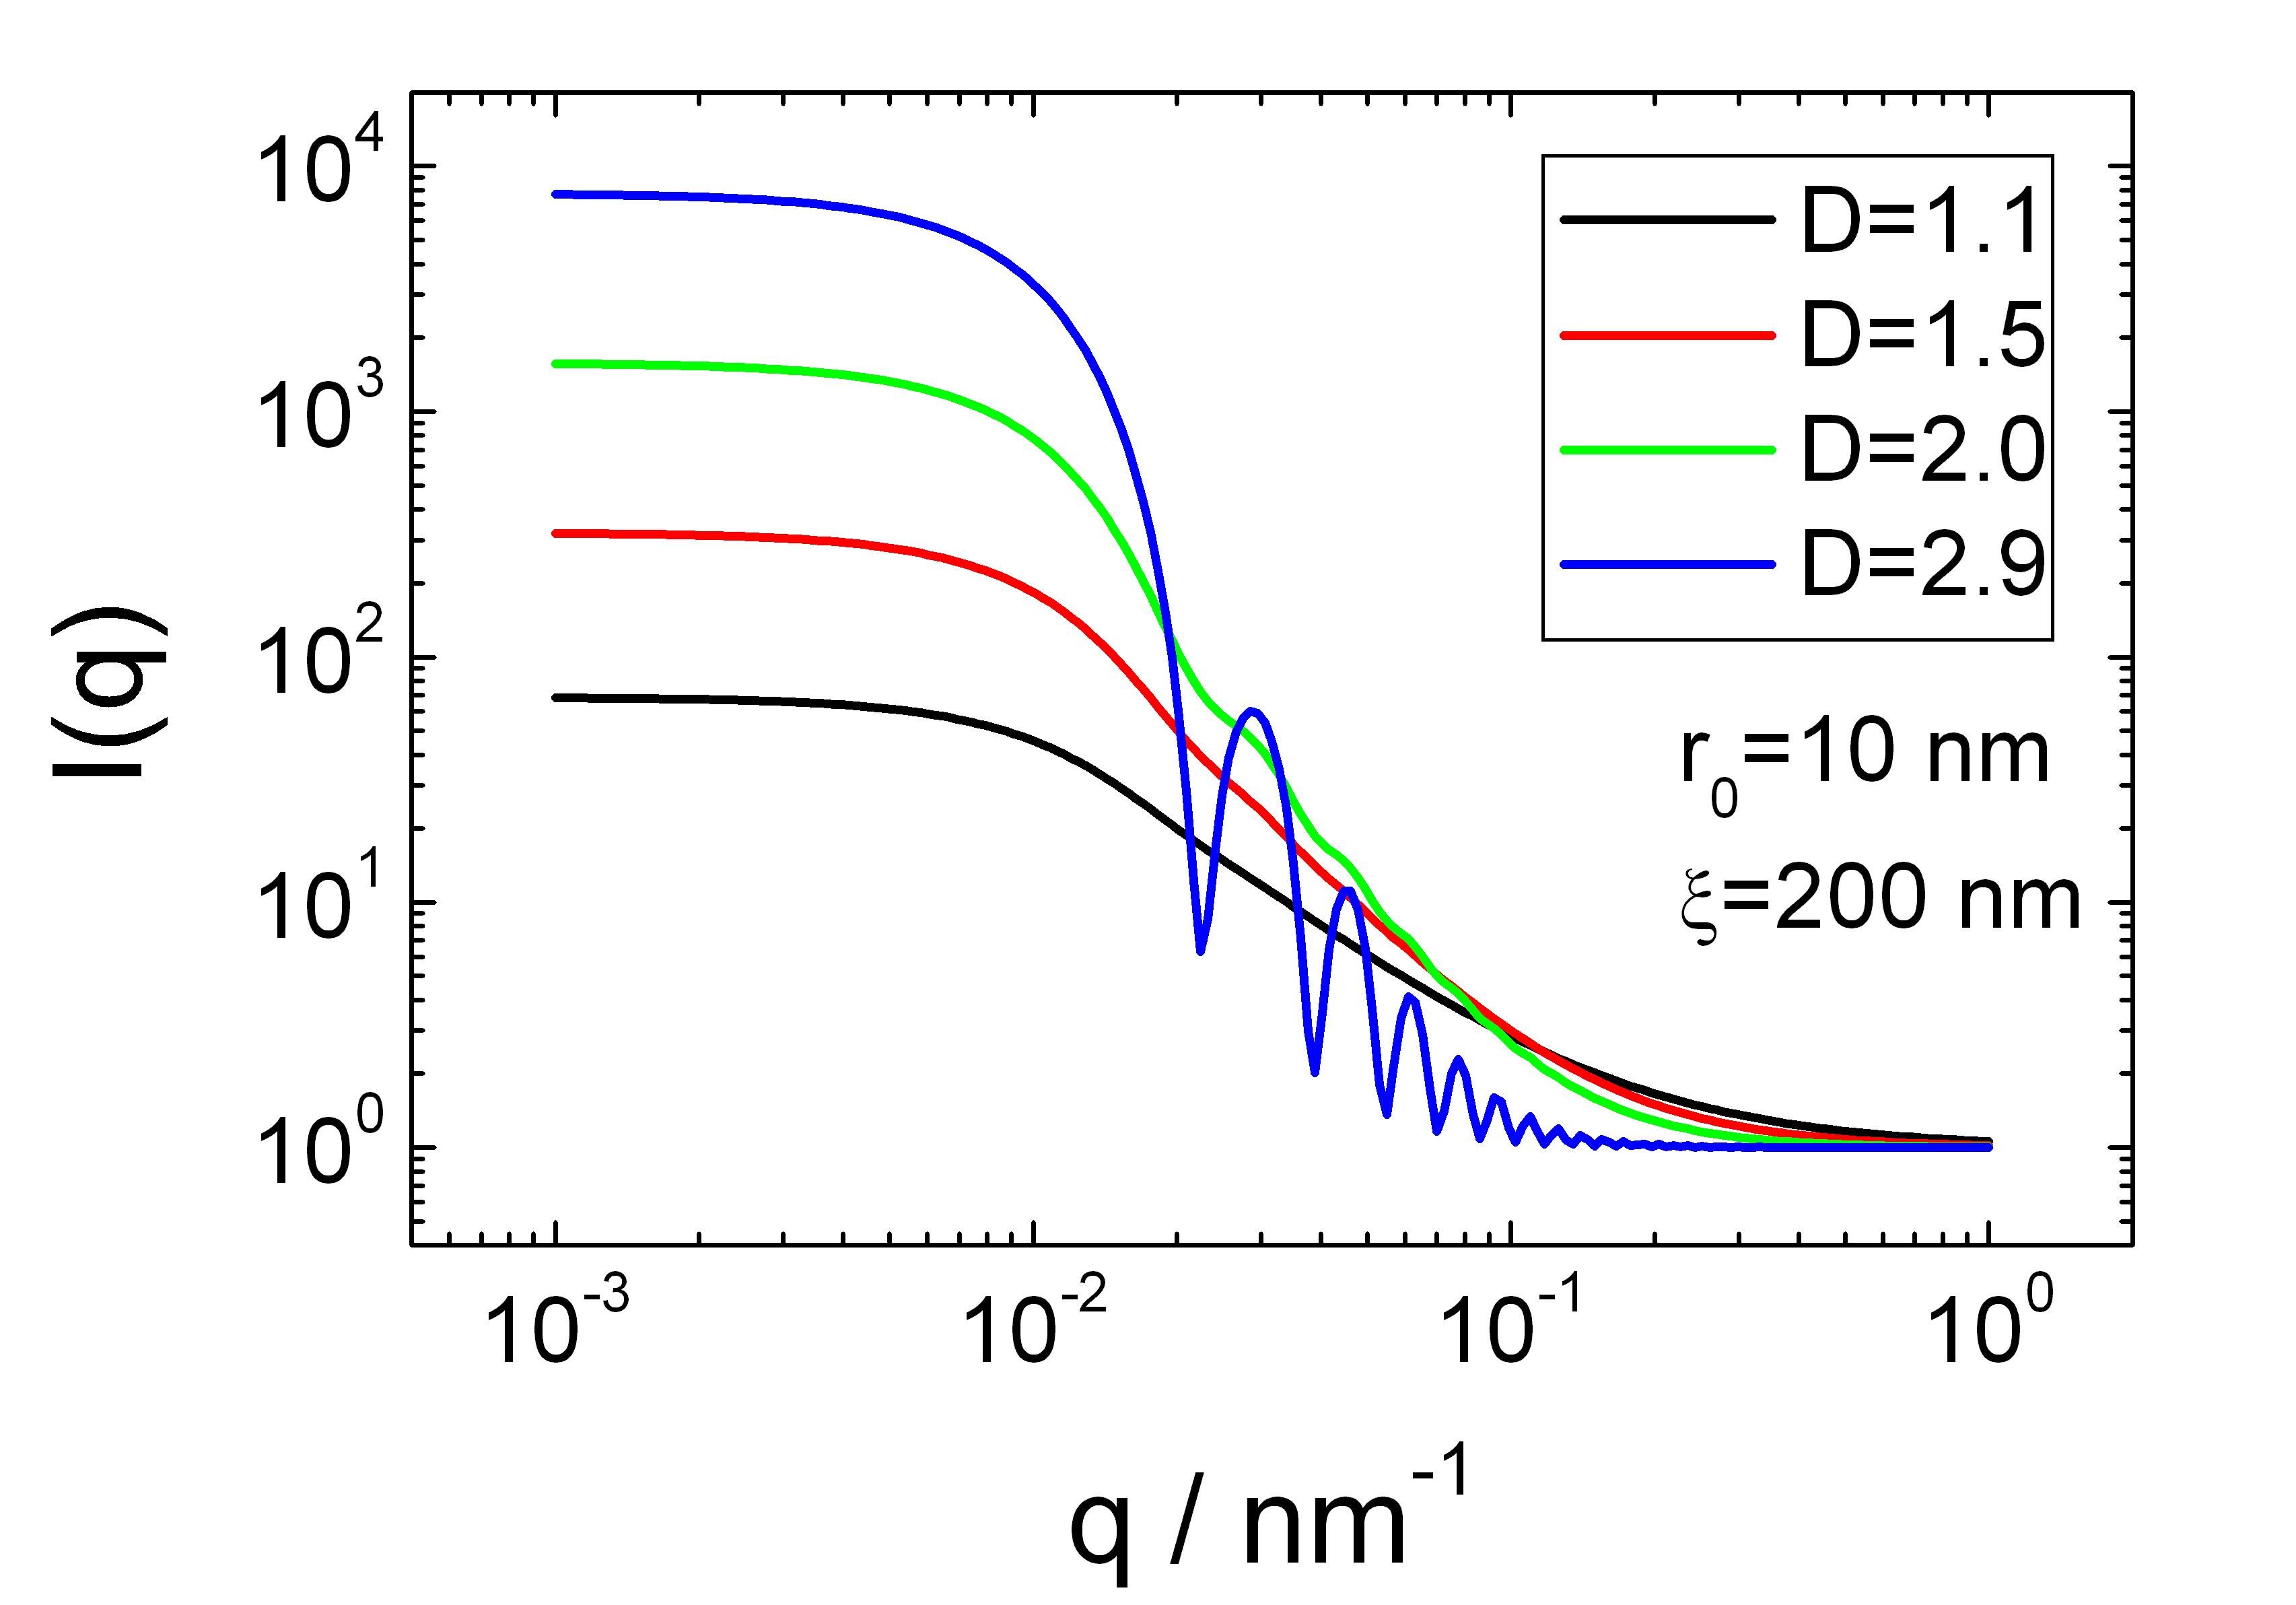
\includegraphics[width=0.768\textwidth,height=0.488\textwidth]{../images/structure_factor/MassFractals/SQOverlapSphCutOff.png}
\end{center}
\caption{Structure factor of a mass fractal with a
cut-off function $h_\text{OverlapSph}(r,\xi) = \left(1+\frac{r}{4\xi}\right)\left(1-\frac{r}{2\xi}\right)^2$ for $r\leq 2\xi$.}
\label{fig:SQGaussCutOff}
\end{figure}

%%%%%%%%%%%%%%%%%%%%%%%%%%%%%%%%%%%%%%%%%%%%%%%%%%%%%%%%%%%%%%%%%%%%%%%%%%%%
\clearpage
\section{Other Structure Factors}

\subsection{Hayter-Penfold RMSA \cite{Hayter1981,Hansen1982}}

This is the structure factor for a system of charged, spheroidal objects in a dielectric
medium. When
combined with an appropriate form factor (such as sphere, core+shell, ellipsoid etc.),
this allows for inclusion of the interparticle interference effects due to screened
coulomb repulsion between charged particles.
The salt concentration, is used to compute the ionic strength of the solution which
in turn is used to compute the Debye screening length. At present there is no provision
for entering the ionic strength directly nor for use of any multivalent salts. The
counterions are also assumed to be monovalent.



\hspace{1pt}\\
\underline{Input Parameters for model \texttt{Hayter Penfold RMSA}:}\\
\begin{description}
\item[\texttt{RHS}] hard sphere radius $R_{HS}$ of particles in [nm].
\item[\texttt{Z}] charge of particle in units of the charge of an electron $e=?1.602 176 53 \times 10^{?19} \mathrm{C}$
\item[\texttt{eta}] volume fraction $\eta$ of particles
\item[\texttt{T}] sample temperature $T$ in Kelvin
\item[\texttt{salt}] monovalent salt concentration in [M]
\item[\texttt{eps\_r}] dielectric constant $\epsilon_r$ of solvent
\end{description}

%\vspace{5mm}
%\noindent REFERENCE\\
%1. JP Hansen and JB Hayter "A rescaled MSA structure factor for dilute charged
%colloidal dispersions" Molecular Physics 46, 651-656 (1982).\\
%2. JB Hayter and J Penfold "An analytic structure factor for macroion solutions"
%Molecular Physics 42, 109-118 (1981)

%%%%%%%%%%%%%%%%%%%%%%%%%%%%%%%%%%%%%%%%%%%%%%%%%%%%%%%%%%%%%%%%%%%%%%%%%%%%

\clearpage
\subsection{MacroIon}

\begin{subequations}
\begin{align}
ETA &= \text{volume fraction} \\
AK &= \kappa \sigma = \text{inv. screening length times diameter} \\
\kappa &=\sqrt{ e^2/(\epsilon \epsilon_0 k_B T)*(\rho_c+2 \rho_s) }\\
\rho_c &= \text{density of counterions} = \rho_\text{colloids} Z \\
\rho_s &= \text{density of salt cations or anions} \\
GEK &=\text{charge}^2/( \pi k_B T \epsilon \epsilon_0 \sigma (2+AK)^2)\\
\text{charge} &= \text{Ladung eines Kolloids} = e Z\\
S=ETA^{1./3} &= \text{scaling factor for rescaled MSA (RMSA)}\\
GAMK&=2*S*GEK*\exp(AK-AK/S).
\end{align}
\end{subequations}

%%%%%%%%%%%%%%%%%%%%%%%%%%%%%%%%%%%%%%%%%%%%%%%%%%%%%%%%%%%%%%%%%%%%%%%%%%%%

\clearpage
\subsection{Critical Scattering}

\BE S_\text{crit}(Q)=1+\frac{\kappa}{1+\zeta^2Q^2} \EE $\zeta$:
correlation length, $\kappa$: scaling factor


%%%%%%%%%%%%%%%%%%%%%%%%%%%%%%%%%%%%%%%%%%%%%%%%%%%%%%%%%%%%%%%%%%%%%%%%%%%%

\subsection{Correlation Hole}
\BE S_\text{corr. hole}(Q,h,\eta)=1+\eta \Phi(Qh) \EE $\Phi(x) =
3\frac{\sin(x)-x\cos(x)}{x^3}$ $\eta$: volume fraction, $h$: hole
radius

%%%%%%%%%%%%%%%%%%%%%%%%%%%%%%%%%%%%%%%%%%%%%%%%%%%%%%%%%%%%%%%%%%%%%%%%%%%%

\subsection{Random Distribution Model}

\BE S_\text{RDM}(Q) =
\frac{1}{1+8\frac{V_{ca}/V_p}\epsilon\Phi(x)} \EE
$x = 2QR_{ca}$ \\
$V_{ca} = \frac{4}{3}\pi R_{ca}^3$ \\
$V_p  = \frac{4}{3}\pi R^3/f_p$ \\
$\Phi(x) = 3\frac{\sin(x)-x\cos(x)}{x^3}$\\
~\\


\subsection{Local Order Model}

\BE S_\text{LOM}(Q) = 1+4\frac{\sin(QD)}{QD}-z\Phi(x); \EE
$x = \alpha Q D$\\
$\Phi(x) = 3\frac{\sin(x)-x\cos(x)}{x^3}$

%%%%%%%%%%%%%%%%%%%%%%%%%%%%%%%%%%%%%%%%%%%%%%%%%%%%%%%%%%%%%%%%%%%%%%%%%%%%

\subsection{Cylinder(PRISM)}

\BE S_\text{Cyl,PRISM} = \frac{1}{1+\nu C_q P_{15}} \EE
$x = 2QR$ \\[3mm]
$x_{P15} = Q(L-2R)$ \\[3mm]
$\displaystyle P_{15} = 2\frac{\text{Si}(x_{P15})}{x_{P15}} - 4\frac{\sin^2(x_{P15}/2)}{x_{P15}^2}$ \\[3mm]
$\displaystyle C_q = 3\frac{\sin(x)-x\cos(x)}{x^3}$ \\

%%%%%%%%%%%%%%%%%%%%%%%%%%%%%%%%%%%%%%%%%%%%%%%%%%%%%%%%%%%%%%%%%%%%%%%%%%%%

\clearpage
\subsection{Voigt Peak} ~\\

In spectroscopy, the Voigt profile is a spectral line profile
named after Woldemar Voigt and found in all branches of
spectroscopy in which a spectral line is broadened by two types of
mechanisms, one of which alone would produce a Doppler profile,
and the other of which would produce a Lorentzian profile. All
normalized line profiles can be considered to be probability
distributions. The Doppler profile is essentially a normal
distribution and a Lorentzian profile is essentially a Cauchy
distribution. Without loss of generality, we can consider only
centered profiles which peak at zero. The Voigt profile is then
the convolution of a Lorentzian profile and a Doppler profile:
\begin{subequations}
\begin{align}
V(x\vert\sigma,\gamma)& = \int_\infty^\infty D(x'\vert\sigma) \,
                                            L(x-x'\vert\gamma)\, dx'
\end{align}
where $x$ is frequency from line center, $D(x\vert\sigma)$ is the
centered Doppler profile:
\begin{align}
D(x\vert\sigma) & = \frac{e^{-x^2/2\sigma^2}}{\sigma\sqrt{2\pi}}
\end{align}
and $L(x\vert\gamma)$ is the centered Lorentzian profile:
\begin{align}
L(x\vert\gamma) & = \frac{\gamma}{\pi(x^2+\gamma^2)} .
\end{align}
The defining integral can be evaluated as:
\begin{align}
V(x) & = \frac{\Re[w(z)]}{\sigma\sqrt{2\pi}}
\end{align}
where $\Re[w(z)]$ is the real part of the complex error function
of $z$ and
\begin{align}
z = \frac{x+i\gamma}{\sigma\sqrt{2}}
\end{align}
\begin{align}
S_{\text{Voigt}}(Q,Q_m,A,\sigma,\gamma,c_0) = A \,\,
V(Q-Q_m\vert\sigma,\gamma)+c_0
\end{align}
\end{subequations}

\chapter{Numerical solutions of the Ornstein Zernike equations}

 During an internship project in summer 2013 Evgeniy
Ponomarev has implemented the core routine for solving the Ornstein
Zernike equations. This algorithm numerically calculates structure
factors $S(q)$, radial distribution functions $g(r)$ and direct
correlation functions $c(r)$ of a systems with known pair
interaction potential $U(r)$.
\section{Background}
The central part of this package is iterative solution of
Ornstein-Zernike equation
\cite{Naegele2004,Henderson2000,Hansen2013,Bomont2008,Caccamo1996}:
\begin{align}\label{eq:oz_h12}
    h(\mathbf{r}_{12})&=c(\mathbf{r}_{12})+ \int c(\mathbf{r}_{13}) \rho(\mathbf{r}_3) h(\mathbf{r}_{32})
    d\mathbf{r}_3 + \cdots
\end{align}
where $h(\mathbf{r}_{12})$ is the total correlation function,
$c(\mathbf{r}_{12})$ the direct correlation function (direct effect
of particle 1 on particle 2), $c(\mathbf{r}_{13})$ the in direct
correlation function describing the effect of particle 1 on particle
3 which influences particle 2, and $\rho$ the particle number
density of the colloids, molecules, or atoms that form the liquid.
If the fluid is uniform and isotropic, the Ornstein�Zernike relation
becomes
\begin{align}\label{eq:ozh(r)}
    h(r)&=c(r)+ \rho \int c(\abs{\mathbf{r}-\mathbf{r}'})  h(r')
    d\mathbf{r}' \\
    &= c(r) + \gamma(r) \label{eq:ozgamma(r)}
\end{align}
The basic idea of this equation is that total correlation between
positions of two particles is a combination of their direct and
indirect (through neighboring particles) interactions. The first
contribution to $h(r)$ is the direct correlation function $c(r)$
that represents the correlation between a particle of a pair with
its closest neighbor separated by a distance $r$. The second
contribution is the indirect correlation function $\gamma(r)$, which
represents the correlation between the selected particle of the pair
with the rest of the fluid constituents.

 $g(r)$ is known as the radial or pair distribution  function, which measures the
probability that given a particle at the origin, another particle of
the fluid can be found at a distance $r$ from it. When the distance
separating a pair of particles tends to infinity, the correlations
vanish and $g(r)$ tends to 1. This means that the total correlation
function defined as $h(r)=g(r)-1$ tends to 0. The Fourier transform
$\mathscr{F} \{\}$ of $g(r)$ and $h(r)$ are directly related to the
structure factor $S(q)$ that is experimentally measurable by x-ray
or neutron scattering
\begin{align}
S(q)&=1+\rho \int
\left[g(r)-1\right]\exp\left(-\imath\mathbf{q}\cdot
\mathbf{r}\right) d\mathbf{r}
\end{align}
and
\begin{align}
S(q) &= 1+ \rho  \tilde{h}(q)
\end{align}
where $\tilde{h}(q)=\mathscr{F} \left\{h(r)\right\}$  is the Fourier
transform of the total correlation function $h(r)$, so that
\begin{align}
\tilde{h}(q) &= \int h(r) \exp\left(-\imath\mathbf{q}\cdot
\mathbf{r}\right) d\mathbf{r}
\end{align}
Via inverse Fourier transform $\mathscr{F}^{-1} \{\}$ of the
structure factor the pair correlation function is obtained
\begin{align}
\rho \left[ g(r)-1\right] &=\mathscr{F}^{-1} \left\{S(q)-1\right\} =
\frac{1}{(2\pi)^3} \int \left( S(q)-1
\right)\exp\left(\imath\mathbf{q}\cdot \mathbf{r}\right) d\mathbf{q}
\end{align}
As for $g(r)$ also the direct correlation function $c(r)$ can be, in
principle, derived from experiment as
\begin{align}
\rho c(r) &= \frac{1}{(2\pi)^3} \int \left(1-\frac{1}{S(q)}\right)
\exp\left(\imath\mathbf{q}\cdot \mathbf{r}\right) d\mathbf{q}
\end{align}
or
\begin{align}
S(q) &= \frac{1}{1+\rho \tilde{c}(q)} \label{eq:ozSq}
\end{align}

By Fourier transformation of eq.\ \ref{eq:ozh(r)}, one obtains
\begin{align}
\tilde{h}(q) &= \frac{\tilde{c}(q)}{1-\rho\tilde{c}(q)}
\label{eq:ozhq}
\end{align}
where $\tilde{c}(q)=\mathscr{F}\left\{c(r)\right\}$ is the Fourier
Transform of $c(r)$. In order to determine the two correlation
functions $h(r)$ and $c(r)$ for a given pair potential $U(r)$, eq.\
\ref{eq:ozh(r)} must be supplemented by an auxiliary closure
relation. Furthermore the Fourier transform of eq.\
\ref{eq:ozgamma(r)} in combination eq.\ \ref{eq:ozhq} allows to
write the Fourier transform of the indirect correlation function as
\begin{align}
\mathscr{F} \left\{\gamma(r)\right\} &= \tilde{\gamma}(q)  =
\tilde{h}(q) - \tilde{c}(q) =
\frac{\rho\tilde{c}^2(q)}{1-\rho\tilde{c}(q)} \label{eq:ozg(q)}
\end{align}


 The closure is not complete as long the bridge function is
unknown. Even though the bridge function is exactly defined the
function is an unknown function of interparticle distance and only
approximations can be given. The direct correlation function can be
written in terms of the indirect correlation function, the
inetraction potential and the bridge function as
\begin{align}\label{eq:ozclosure}
c(r)&= \exp\left[ -\beta U(r) +\gamma(r)+B(r)\right] - \gamma(r)-1 \\
    &= g(r)- \gamma(r)-1 \nonumber \\
\mbox{and } h(r)+1=g(r)&= \exp\left[ -\beta U(r)
+\gamma(r)+B(r)\right] \label{eq:ozg(r)}
\end{align}
where $U(r)$ is the pair interaction potential, $\beta=1/(k_B T)$
the inverse temperature, with $k_B$ being Boltzmann�s constant, $T$
is the absolute temperature, $\gamma(r)$ being the indirect
correlation function and $\rho$ is the number density of the
molecules or atoms that form the liquid. $B(r)$ is the bridge
function. The analytic expression of $B(r)$ is, in general, unknown.
Unfortunately, the bridge function has to be approximated in
practice. Though a number of theoretical and simulation procedures
have been derived in recent years in order to get an approximate
estimate of $B(r)$ for different fluid models, the exact bridge
function is not known for any system.

The numerical iterative procedure to solve the Ornstein Zernike
equation \ref{eq:ozh(r)} together with the closure equation
\ref{eq:ozclosure} is the following:
\begin{enumerate}
\item Guess a starting value for $\gamma(r)$, e.q. set $\gamma(r)\equiv 0$
\item Calculate a bridge function. Many different theories how to calculate
the bridge function have been published. A few of them are described
in the next section. The bridge function is often expressed in terms
of the known potential $U(r)$ and the indirect correlation function
$\gamma(r)$, which needs to be determined.
\item Calculate the direct correlation function according to eq.\
\ref{eq:ozclosure}.
\item Calculate the Fourier transform $\tilde{c}(q)$ of the direct correlation
function.
\item Use eq.\ \ref{eq:ozg(q)} to get $\tilde{\gamma}(q)$.
\item Calculate the inverse Fourier transform of $\tilde{\gamma}(q)$
to get the new guess for $\gamma(r)$.
\item Compare the new gess of the indirect correlation function with the one used in step 1,
i.e. compare $\gamma_\text{new}(r)$ and $\gamma_\text{old}(r)$ at each grid point.
If $\Norm{\gamma_\text{new}(r)-\gamma_\text{old}(r)}/\Norm{\gamma_\text{new}(r)} < \epsilon_\text{rel}$
the solution has been found otherwise go back to the first step by using the new $\gamma_\text{new}(r)$ as a
starting value and repeat the loop until convergence.
\item When the iteration loop has converged calculate $S(q)$ and
$g(r)$ according to eq.\ \ref{eq:ozSq} and eq.\ \ref{eq:ozg(r)}.
\end{enumerate}
In actual practice, it turns out that this simple iteration doesn�t converge very rapidly and
can have oscillations. One can improve the convergence rate in several ways:
\begin{enumerate}
\item Introduction of  Broyles mixing; specifically, before repeating the iteration, let
$\gamma_\text{old}(r) = \alpha \gamma_\text{new}(r) + (1 -\alpha)\gamma_\text{old}(r)$
where the mixing parameter $\alpha \in [0;1]$. A typiclal staring value would be 0.5.
\item One can slowly change one of the physical parameters, e.g., density or temperature. For
example, if one want a high density solution, one can first obtain a low density one, and
use it as the initial guess for the high density one. Clearly, this may have been done in several
stages. As long the number of grid points is not changed \SASfit uses as starting values the result
of the previous calculation as initialisation values.
\end{enumerate}

\section{Numerical implementation of the iterative algorithm in SASfit}
In the above algorithm to iteratively solve the Ornstein Zernike
equation two Fourier transforms have to be performed:
\begin{align}
c(r) & \xrightarrow{\mathscr{F}\{\}} \tilde{c}(q)  \mbox{ step 4} \\
\tilde{\gamma}(q) & \xrightarrow{\mathscr{F}^{-1}\{\}} \gamma(r) \mbox{ step 6}
\end{align}
A we assume that the system is isotropic, i.e. $c(r)$ and $\gamma(r)$ are only functions
of the modulus of $\abs{\mathbf{r}}=r$ the Fourier transforms can be written as
\begin{align}
\tilde{c}(q) &= \int c(r) \exp\left(- \imath\mathbf{q}\cdot \mathbf{r} \right) d\mathbf{r}
              = \int_0^\infty 4\pi r^2 c(r)              \frac{\sin(qr)}{qr}  dr \\
\gamma(r)    &= \frac{1}{(2\pi)^3}
                \int \tilde{\gamma}(q) \exp\left(\imath\mathbf{q}\cdot \mathbf{r}\right) d\mathbf{q}
              = \frac{1}{(2\pi)^3}
                \int_0^\infty 4\pi q^2 \tilde{\gamma}(q) \frac{\sin(qr)}{qr}  dq
\end{align}
To calculate these transforms numerically on a discrete grid of points
one has to substitute the integration by a summation. Herby $\int_0^\infty dr$ is replaced by
$\sum_{j=0}^{N_p-1} \Delta r$, $r_j=(j+1)\Delta r$, $q_j=(j+1)\Delta q$, and $\int_0^\infty dq$ is replaced by
$\sum_{j=0}^{N_p-1} \Delta q$. The step width $\Delta r$ in real space has to be defined by the user as well
as the number of grid points $N_p$. The step width in reciprocal space is than obtained by
$\Delta q=\frac{\pi}{(N_p+1)\Delta r}$.
It is important to mention that values of first elements of $r_{i=0}$ and $k_{i=0}$ arrays equal $\Delta r$
and $\Delta q$, respectively ($r_0=\Delta r, q_0=\Delta q$).
\begin{align}
\tilde{c}_i &=                   \frac{4\pi \Delta r^2}{(i+1)\Delta q} \sum_{j=0}^{N_p-1}              c_j (j+1) \sin\left(\frac{\pi(j+1)(i+1)}{N_p+1}\right) \\
\gamma_i    &= \frac{1}{(2\pi)^3}\frac{4\pi \Delta q^2}{(i+1)\Delta r} \sum_{j=0}^{N_p-1} \tilde{\gamma}_j (j+1) \sin\left(\frac{\pi(j+1)(i+1)}{N_p+1}\right)
\end{align}
For calculating the Fourier transformation the library \texttt{FFTW} for fast fourier transformation
\cite{FFTW05,FFTW97} has been used. The library supplies a discrete sin transformation (type-I DST)
named \verb"FFTW_RODFT00" which doing the transformation
\begin{align}
Y_k &= 2 \sum_{j=0}^{N_p-1} X_j \sin\left(\frac{\pi(j + 1)(k + 1)}{N_p + 1}\right)
\end{align}
The unnormalized inverse of \verb"FFTW_RODFT00" is \verb"FFTW_RODFT00" itself.
The same routine can be used for both transformations.

\section{Thermodynamic Parameters and Consistency Tests}
The excess internal energy per particle is given by
\begin{align}
\frac{E_\text{ex}}{N} &= 2\pi\rho \int g(r) U(r) r^2 \;dr
\end{align}
and the virial pressure can be written as
\begin{align}
\frac{\beta P}{\rho} &= 1=\frac{2}{3} \beta\pi\rho\int g(r) r^3 \frac{dU(r)}{dr} dr
\end{align}
where $\rho= N/V$ is the average number density of particles in the system.

\section{Classical Closures}
\subsection{Hypernetted-chain(HNC) approximation}
~\\
The simplest assumption for completing the closure relation
\ref{eq:ozclosure} is by setting the bridge function to zero
\begin{align} \label{eq:ozBHNC}
B_\text{HNC}(r) &\equiv 0 \\
g(r)&=\exp\left[ -\beta U(r) +\gamma(r)\right]
\end{align}
The HNC equation is a special case insofar as it corresponds to a
well-defined free-energy functional, and differentiation of that
free energy with respect to volume can be shown to give the same
result as the virial equation. The energy and virial routes to the
equation of state are therefore equivalent.

\subsection{Percus-Yevick (PY) approximation}
~\\
\begin{align} \label{eq:ozBHNC}
B_\text{PY}(r) &=\gamma(r)-\ln\left[\gamma(r)-1\right] \\
g(r)&= \exp\left[ -\beta U(r)\right]\left(1 +\gamma(r)\right)
\end{align}
The PY equation proves to be more successful than the HNC
approximation when the potential is strongly repulsive and short
ranged. The PY equation is of particular interest in the theory of
simple liquids because it is soluble analytically in the important
case of the hard-sphere fluid.

\subsection{Mean Spherical Approximation (MSA)}
\begin{alignat}{2}
g(r) &=  0 &\mbox{ for } \beta U(r) = +\infty \\
c(r) &= -\beta U(r) &\mbox{ for } \beta U(r) \neq +\infty
\end{alignat}

\section{Verlet-type Closures}

\subsection{Verlet Approximation}
\begin{align} \label{eq:ozBHNC}
B_\text{Verlet}(r)
&=\frac{-\gamma^2(r)}{2\left(1+\frac{4}{5}\gamma(r)\right)}
\end{align}

\subsection{Choudhury-Gosh (CG) Approximation}
\begin{align}
B_\text{CG}(r) &=
\frac{-\gamma^{*2}}{2\left(1+\alpha\gamma^*(r)\right)}
\end{align}

\subsection{Duh-Haymet (DH) Approximation}
\begin{align}
B_\text{DH}(r) &=
\frac{-\gamma^{*2}(r)}{2\left[1+\frac{5\gamma^*(r)+11}{7\gamma^*(r)+9}\gamma^*(r)\right]}
\end{align}

\section{Martynov-Sarkisov-type Closures}

\subsection{Martynov-Sarkisov (MS) Approximation}
\begin{align}
B_\text{MS}(r) &= \left[1+2\gamma(r)\right]^{1/2}-1-\gamma(r)
\end{align}

\subsection{Ballone, Pastore, Galli, and Gazzillo (BPGG) approximations}
\begin{align}
B_\text{BPGG}(r) &= \left[1+s\gamma(r)\right]^{1/s}-1-\gamma(r)
\end{align}

\subsection{Vompe-Martynov (VM) Approximation}
\begin{align}
B_\text{VM}(r) &= \sqrt{1+2\gamma^*(r)}-1-\gamma^*(r)
\end{align}

\subsection{Chapentier-Jakse' semiempirical extention of the VM Approximation (CJ-VM)}
\begin{align}
B_\text{CJ-VM}(r) &= \frac{1}{2\alpha}\left[\sqrt{1+4\alpha
\gamma^*(r)}-1-2\alpha\gamma^*(r) \right]
\end{align}

\subsection{Bomont, Bretonnet (BB) Approximation}
\begin{align}
B_\text{BB}(r) &=
\sqrt{1+2\gamma^*(r)+f*\gamma^{*2}(r)}-1-\gamma^*(r)
\end{align}

\section{Phenomenological Closures}

\subsection{Reference HNC Approximation}


\section{Mixed Closure' theories }
\subsection{Roger-Young (RY) closure}
\begin{align}
B_\text{RY}(r) &= \ln
\left[1+\frac{\exp\left[f(r)\gamma(r)\right]-1}{f(r)}\right]-\gamma(r)
\end{align}

\subsection{"Soft core" MSA (SMSA) Approximation}
\begin{align}
B_\text{SMSA}(r) &= \ln \left[1+\gamma^*(r)\right]-\gamma^*(r)
\end{align}

\subsection{HNC-SMSA (HMSA) Approximation}
\begin{align}
B_\text{HMSA}(r) &= \ln
\left[1+\frac{\exp\left[f(r)\gamma^*(r)\right]-1}{f(r)}\right]-\gamma^*(r)
\end{align}
